 %	Main Document

\documentclass[
	12pt,
	BCOR=5mm,
	DIV=12,
	headinclude=on,
	footinclude=off,
	parskip=half,
	bibliography=totoc,
	listof=entryprefix,
	toc=listof,
	pointlessnumbers,
	plainfootsepline]{scrreprt}

% include configuration file
% !TEX root =  master.tex

% language, font, colors
\usepackage[ngerman]{babel}
\usepackage[utf8]{inputenc}
\usepackage[german=quotes]{csquotes} 	% correct quotes using \enquote{}
\usepackage[T1]{fontenc}
\usepackage{lmodern} % latin modern font
\usepackage[onehalfspacing]{setspace}
\usepackage{xcolor}

% hyperlinks
\PassOptionsToPackage{hyphens}{url}\usepackage[hidelinks=true]{hyperref}

% commands for author and title
\newcommand{\TitelDerArbeit}[1]{\def\DerTitelDerArbeit{#1}\hypersetup{pdftitle={#1}}}
\newcommand{\AutorDerArbeit}[1]{\def\DerAutorDerArbeit{#1}\hypersetup{pdfauthor={#1}}}
\newcommand{\Firma}[1]{\def\DerNameDerFirma{#1}}
\newcommand{\Kurs}[1]{\def\DieKursbezeichnung{#1}}


%\usepackage{microtype}% verbesserter Randausgleich
%\setlength\emergencystretch{1em}
% correct superscripts
\usepackage{fnpct}

\usepackage{footnote}
\usepackage{rotating}

% calc
\usepackage{calc} % Used for extra space below footsepline

% bibliography settings
% author-year-style with footnotes (Chicago)
\usepackage[backend=biber, autocite=footnote, style=authoryear, dashed=false]{biblatex}
\AdaptNoteOpt\footcite\multfootcite
\AdaptNoteOpt\autocite\multautocite

\DefineBibliographyStrings{ngerman}{  % change \ua to et al. (german only!)
	andothers = {{et\,al\adddot}},
}


% Command to output section title headings
\newcommand{\cvsect}[1]{% The only parameter is the section text
	\vspace{\baselineskip} % Whitespace before the section title
	\colorbox{black}{\textcolor{white}{\MakeUppercase{\textbf{#1}}}}\\% Section title
}

\newcounter{barcount}

% Environment to hold a new bar chart
\newenvironment{barchart}[1]{ % The only parameter is the maximum bar width, in cm
	\newcommand{\barwidth}{0.35}
	\newcommand{\barsep}{0.55}
	
	% Command to add a bar to the bar chart
	\newcommand{\baritem}[2]{ % The first argument is the bar label and the second is the percentage the current bar should take up of the total width
		\pgfmathparse{##2}
		\let\perc\pgfmathresult
		
		\pgfmathparse{#1}
		\let\barsize\pgfmathresult
		
		\pgfmathparse{\barsize*##2/5}
		\let\barone\pgfmathresult
		
		\pgfmathparse{(\barwidth*\thebarcount)+(\barsep*\thebarcount)}
		\let\barx\pgfmathresult
		
		\filldraw[fill=none, draw=black!] (0,-\barx) rectangle (5,-\barx-\barwidth);
		\filldraw[fill=black!90, draw=black!90] (0,-\barx) rectangle (\barone,-\barx-\barwidth);
		
		\node [label=180:{\textcolor{black}{##1: ##2/5}}] at (0,-\barx-0.175) {};
		\addtocounter{barcount}{1}
	}

	\newcommand{\baritemNL}[2]{ % The first argument is the bar label and the second is the percentage the current bar should take up of the total width
		\pgfmathparse{##2}
		\let\perc\pgfmathresult
		
		\pgfmathparse{#1}
		\let\barsize\pgfmathresult
		
		\pgfmathparse{\barsize*##2/5}
		\let\barone\pgfmathresult
		
		\pgfmathparse{(\barwidth*\thebarcount)+(\barsep*\thebarcount)}
		\let\barx\pgfmathresult
		
		\filldraw[fill=none, draw=black!] (0,-\barx) rectangle (5,-\barx-\barwidth);
		\filldraw[fill=black!90, draw=black!90] (0,-\barx) rectangle (\barone,-\barx-\barwidth);
		
		\node [label=180:{}] at (0,-\barx) {};
		\addtocounter{barcount}{1}
	}

	\begin{tikzpicture}
	\setcounter{barcount}{0}
}{
	\end{tikzpicture}
	\vspace{0.3cm}
}

\usepackage{tikz} % Required for creating the plots
\usetikzlibrary{shapes, backgrounds}
\tikzset{x=1cm, y=1cm} % Default tikz units

%%% Uncomment the following lines to support hard URL breaks in bibliography 
%\apptocmd{\UrlBreaks}{\do\f\do\m}{}{}
%\setcounter{biburllcpenalty}{9000}% Kleinbuchstaben
%\setcounter{biburlucpenalty}{9000}% Großbuchstaben

\setlength{\bibparsep}{\parskip}	% add some space between biblatex entries in the bibliography
\addbibresource{bibliography-martin.bib}	% add file bibliography.bib as biblatex resource
\addbibresource{bibliography-rene.bib}	% add file bibliography.bib as biblatex resource
\addbibresource{bibliography-sascha.bib}	% add file bibliography.bib as biblatex resource
\addbibresource{bibliography-niko.bib}	% add file bibliography.bib as biblatex resource
\addbibresource{bibliography-julian.bib}	% add file bibliography.bib as biblatex resource
\addbibresource{bibliography-erik.bib}	% add file bibliography.bib as biblatex resource
% footnotes (count footnotes over chapters)
\usepackage{chngcntr}
\counterwithout{footnote}{chapter}

% acronyms
\makeatletter
\usepackage[printonlyused]{acronym}
\@ifpackagelater{acronym}{2015/03/20}
  {%
    \renewcommand*{\aclabelfont}[1]{\textbf{\textsf{\acsfont{#1}}}}
  }%
  {%
  }%
\makeatother

% listings
\usepackage{listings}
\renewcommand{\lstlistingname}{Quelltext}
\renewcommand{\lstlistlistingname}{Quelltextverzeichnis}

%% More configuration for listings is in configlistings.tex %%


% extra packages
\usepackage{graphicx}			% use various graphics formats
\usepackage[german]{varioref}	% nicer references \vref
\usepackage{caption}			% better captions
\usepackage{booktabs}			% nicer tabs
\usepackage{array}
\usepackage{pdfpages}			% for signed ewerkl
%\usepackage{import}				% better import of section in several files
\usepackage{subfigure}

% table stuff
\newcolumntype{L}[1]{>{\raggedright\let\newline\\\arraybackslash\hspace{0pt}}m{#1}} % combines l and p
\newcolumntype{C}[1]{>{\centering\let\newline\\\arraybackslash\hspace{0pt}}m{#1}} % combines c and p
\newcolumntype{R}[1]{>{\raggedleft\let\newline\\\arraybackslash\hspace{0pt}}m{#1}} % combines r and p

% funktioniert aktuell nicht wie normal -> muss man nochmal drüber schauen.. oder ersetzen
\usepackage{tabularx}
\newcolumntype{Y}{>{\centering\arraybackslash}X}
\newcolumntype{b}{X}
\newcolumntype{s}{>{\hsize=.5\hsize\raggedleft\arraybackslash}X}
\newcolumntype{k}{>{\hsize=.5\hsize\arraybackslash}X}
\newcolumntype{r}{>{\raggedright\arraybackslash}X}

% page header/footer
\RequirePackage{scrlfile}
\ReplacePackage{scrpage2}{scrlayer-scrpage}
\RequirePackage[automark,headsepline,footsepline]{scrpage2}
\pagestyle{scrheadings}
\renewcommand*{\pnumfont}{\upshape\sffamily}
\renewcommand*{\headfont}{\upshape\sffamily}
\renewcommand*{\footfont}{\upshape\sffamily}
\renewcommand{\chaptermarkformat}{}
\RedeclareSectionCommand[beforeskip=0pt]{chapter}
\clearscrheadfoot

\ifoot[\rule{0pt}{\ht\strutbox+\dp\strutbox}DHBW Mannheim]{\rule{0pt}{\ht\strutbox+\dp\strutbox}DHBW Mannheim}
\ofoot[\rule{0pt}{\ht\strutbox+\dp\strutbox}\pagemark]{\rule{0pt}{\ht\strutbox+\dp\strutbox}\pagemark}

\ohead{\headmark}

% highlight notes as not yet finished
\newenvironment{note}{\color{gray}}{}

\usepackage{todonotes}
\usepackage{xspace}% http://ctan.org/pkg/xspace
\usepackage{fontawesome5}
\usepackage{float} % !important for figure position

% !TEX root =  master.tex

% colors
\definecolor{javared}{rgb}{0.6,0,0} % for strings
\definecolor{javagreen}{rgb}{0.25,0.5,0.35} % comments
\definecolor{javapurple}{rgb}{0.5,0,0.35} % keywords
\definecolor{javadocblue}{rgb}{0.25,0.35,0.75} % javadoc

\colorlet{jsonPunct}{red!60!black}
\definecolor{jsonBackground}{HTML}{EEEEEE}
\definecolor{jsonDelim}{RGB}{20,105,176}
\colorlet{jsonNumb}{magenta!60!black}

\definecolor{xmlGray}{rgb}{0.4,0.4,0.4}
\definecolor{xmlDarkblue}{rgb}{0.0,0.0,0.6}
\definecolor{xmlCyan}{rgb}{0.0,0.6,0.6}

\definecolor{jsBackground}{RGB}{250,250,255}
\definecolor{jsString}    {RGB}{ 16,160, 60}

\definecolor{cssKeyword}{RGB}{ 10,100,160}
\definecolor{cssClass}  {RGB}{200,120, 10}

% general style
\lstset{
	basicstyle=\ttfamily\footnotesize,
	backgroundcolor=\color{jsBackground},
	numbers=left,
	numberstyle=\scriptsize\color{black},
	stepnumber=1,
	numbersep=10pt,
	showspaces=false,
	showstringspaces=false,
	breaklines=true,
	tabsize=2,
	captionpos=b,
	literate=
	{Ö}{{\"O}}1
	{Ä}{{\"A}}1
	{Ü}{{\"U}}1
	{ß}{{\ss}}1
	{ü}{{\"u}}1
	{ä}{{\"a}}1
	{ö}{{\"o}}1
}

% Java
\lstdefinestyle{lstJava}
{
	language=Java,
	keywordstyle=\color{javapurple}\bfseries,
	stringstyle=\color{javared},
	commentstyle=\color{javagreen},
	morecomment=[s][\color{javadocblue}]{/**}{*/},
	tabsize=1
}

% JSON
\lstdefinelanguage{json}{
	literate=
	*{0}{{{\color{jsonNumb}0}}}{1}
	{1}{{{\color{jsonNumb}1}}}{1}
	{2}{{{\color{jsonNumb}2}}}{1}
	{3}{{{\color{jsonNumb}3}}}{1}
	{4}{{{\color{jsonNumb}4}}}{1}
	{5}{{{\color{jsonNumb}5}}}{1}
	{6}{{{\color{jsonNumb}6}}}{1}
	{7}{{{\color{jsonNumb}7}}}{1}
	{8}{{{\color{jsonNumb}8}}}{1}
	{9}{{{\color{jsonNumb}9}}}{1}
	{:}{{{\color{jsonPunct}{:}}}}{1}
	{,}{{{\color{jsonPunct}{,}}}}{1}
	{\{}{{{\color{jsonDelim}{\{}}}}{1}
	{\}}{{{\color{jsonDelim}{\}}}}}{1}
	{[}{{{\color{jsonDelim}{[}}}}{1}
	{]}{{{\color{jsonDelim}{]}}}}{1}
}

% XML
\lstdefinelanguage{XML}
{
	morestring=[b]",
	morestring=[s]{>}{<},
	morecomment=[s]{<?}{?>},
	stringstyle=\color{xmlGray},
	identifierstyle=\color{xmlDarkblue},
	keywordstyle=\color{xmlCyan},
	morekeywords={xmlns,version,type}
}

% JavaScript
\lstdefinelanguage{JavaScript}
{
	backgroundcolor=\color{jsBackground},
	keywordstyle=\color{blue}\bfseries,
	stringstyle=\color{jsString},
	commentstyle=\color{gray},
	morestring=[b]",
	morecomment=[l][\color{gray}]{//},
	morecomment=[s][\color{gray}]{/*}{*/},
	morekeywords={break,case,const,continue,else,false,for,function,if,in,new,null,switch,this,true,var,while}
}

% HTML
\lstdefinestyle{lstHTML}
{
	language=HTML,
	keywordstyle=\color{blue}\bfseries,
	commentstyle=\color{gray}\itshape,
	morecomment=[s][\color{gray}]{<!--}{-->},
%	stringstyle=\color{jsString}
	escapeinside=``
}

% CSS
\lstdefinestyle{lstCSS}
{
	keywordstyle=\color{cssKeyword}\bfseries,
	commentstyle=\color{gray}\itshape,
	morecomment=[s][\color{gray}]{/*}{*/},
%	morecomment=[s][\color{cssClass}]{.}{ \{},
	alsoletter=-,
	morekeywords={border,background-color}
}

%lstinline
\def\jinline{\lstinline[basicstyle=\ttfamily,keywordstyle={}, language=JAVA]}
\def\sinline{\lstinline[basicstyle=\ttfamily,keywordstyle={}, language=SQL]}

% !TEX root =  master.tex

\newcommand{\authorSG}{Sascha Görnert}
\newcommand{\authorNL}{Niko Lockenvitz}
\newcommand{\authorRF}{Rene Fischer}
\newcommand{\authorEJ}{Erik Jansky}
\newcommand{\authorGP}{Gerrit Pollkläsener}
\begin{document}

% set some information (title, author, ...)
\TitelDerArbeit{Integrationsseminar}
\AutorDerArbeit{\authorSG, \authorRF, \authorMS, \authorEJ, \authorNL, \authorJR}
\Firma{DER Touristik GmbH, Technische Universität Kaiserslautern, SAP SE}
\Kurs{WWI 17 SE B}

\begin{titlepage}

\begin{minipage}{\textwidth}
	\vspace{-2cm}
	\noindent
	
\includegraphics[height=0.1\linewidth]{img/logos/der}
	\hfill
	
\includegraphics[height=0.1\linewidth]{img/logos/tukl}
	\hfill
	
\includegraphics[height=0.1\linewidth]{img/logos/sap}
	\hfill
	
\includegraphics[height=0.1\linewidth]{img/logos/dhbw}
\end{minipage}

\vspace{1em}
\sffamily

\begin{center}
	\textsf{\large{}Duale Hochschule Baden-Württemberg\\[1.5mm] Mannheim}\\[2em]
	\textsf{\textbf{\Large{}Seminararbeit}}\\[3mm]
	\textsf{\textbf{\DerTitelDerArbeit}}\\[1.5cm]
	\textsf{\textbf{\Large{}Studiengang Wirtschaftsinformatik}\\[3mm] \textsf{Studienrichtung Software Engineering}}
	
	\vspace{3em}
	\vfill

	\begin{minipage}{\textwidth}
	
		\begin{tabbing}
			Bearbeitungszeitraum: \hspace{0.85cm}\=\kill
			Verfasser: \> \authorSG, 2716910 \\
			\> DER Touristik GmbH \\
			\> \\
			\> \authorRF, 8703049 \\
			\> Technische Universität Kaiserslautern \\
			\> \\
			\> \authorMS, 8857640 \\
			\> SAP SE \\
			\> \\
			\> \authorEJ, 5980253 \\
			\> SAP SE \\
			\> \\
			\> \authorNL, 1308674 \\
			\> SAP SE \\
			\> \\[1.5mm]
			Kurs: \> \DieKursbezeichnung \\[1.5mm]
			Bearbeitungszeitraum: \> 18.11.2019 -- 09.06.2020
	\end{tabbing}

	\end{minipage}

\end{center}

\end{titlepage}

\pagenumbering{roman}
\normalfont

% table of contents
\clearpage
\pdfbookmark{Inhaltsverzeichnis}{toc-bookmark}
\tableofcontents

% figures
\listoffigures

% tables
%\listoftables

% listings (source code)
\lstlistoflistings

% acronyms
\clearpage
\chapter*{Abkürzungsverzeichnis}
\addcontentsline{toc}{chapter}{Abkürzungsverzeichnis}

\begin{acronym}[A23456789012] % longest acronym for correct indentation
	\acro{A23456789012}{This is just for indentation}

	\acro{AJAX}{Asynchronous JavaScript and \acs{XML}}
	\acro{API}{Application Programming Interface}
	\acro{CRUD}{Create, Read, Update, Delete}
	\acro{CSS}{Cascading Style Sheets}
	\acro{DAO}{Data Access Object}
	\acro{DBMS}{Datenbankmanagementsystem}
	\acro{DOM}{Document Object Model}
	\acro{DTO}{Data Transfer Object}
	\acro{DOM}{Document Object Model}
	\acro{DB}{Datenbank}
	\acro{ER-Modell}{Entity-Relationship-Modell}
	\acro{FSK}{Freiwillige Selbstkontrolle der Filmwirtschaft}
	\acro{HTML}{Hypertext Markup Language}
	\acro{HTTP}{Hypertext Transfer Protocol}
	\acro{HTTPS}{Hypertext Transfer Protocol Secure}
	\acro{IDE}{Integrated Development Environment}
	\acro{JOSE}{\acs{JSON} Object Signing and Encryption}
	\acro{JPA}{Java Persistence \acs{API}}
	\acro{JS}{JavaScript}
	\acro{JSX}{JavaScript \acs{XML}}
	\acro{JPQL}{Java Persistence Query Language}
	\acro{JSON}{JavaScript Object Notation}
	\acro{JWE}{JSON Web Encryption}
	\acro{JWS}{JSON Web Signature}
	\acro{JWT}{JSON Web Token}
	\acro{MVC}{Model-View-Controller}
	\acro{ORM}{Objektrelationaler Mapper}
	\acrodefplural{ORM}{Objektrelationale Mapper}
	\acro{POJO}{Plain Old Java Object}
	\acro{PWA}{Progressive Web App}
	\acrodefplural{PWA}{Progressive Web Apps}
	\acro{QR-Code}{Quick Response Code}
	\acro{RDBMS}{Re\-la\-tio\-nal Database Management System}
	\acro{RFC}{Request for Comments}
	\acro{REST}{Representational State Transfer}
	\acro{SOA}{Service-Oriented Architecture}
	\acro{SPA}{Single-Page-Anwendung}
	\acrodefplural{SPA}{Single-Page-Anwendungen}
	\acro{SQL}{Structured Query Language}
	\acro{URI}{Uniform Resource Identifier}
	\acro{URL}{Uniform Resource Locator}
	\acro{URN}{Uniform Resource Name}
	\acro{UX}{User Experience}
	\acro{UI}{User Interface}
	\acro{XML}{Extensible Markup Language}
\end{acronym}

\ohead{Abkürzungsverzeichnis}

%--------------------------------
% Content
%--------------------------------
\clearpage
\ihead{\chaptername~\thechapter}
\ohead{\headmark}
\pagenumbering{arabic}

\chapter{Einleitung}
\label{c:einleitung}
% !TEX root =  ../../master.tex
\section{Motivation und Zielsetzung}

In der heutigen digitalisierten Welt sind Online-Umfragen ein bewährtes Mittel der Sozialforschung.
Das beste Beispiel hierfür ist das Unternehmen Alphabet Inc., welches durch seine Google-Umfrage-Applikation Android-Nutzern regelmäßig Umfragen unterbreitet und damit nicht nur seine eigene Produkte, sondern auch aktive Sozialforschung betreibt.
Damit auch die \acs{DHBW} Mannheim eine Möglichkeit besitzt, eigene Online-Umfragen ohne die Nutzung von Drittanbieter-Software zu erstellen, um Daten für entsprechende Sozialforschungen zu erheben, soll im Rahmen dieser Seminararbeit eine solche Anwendung entwickelt werden.

Dabei liegt die Zielsetzung in der Gestaltung und Umsetzung einer Applikation, mit der verschiedene Umfragen personalisiert erstellt und ausgewertet werden können.


Zielsetzung der Anwendung ist es, Dozenten zu ermöglichen mittels Umfragen den Studenten eine Möglichkeit zu bieten Gelerntes zu verinnerlichen und Anmerkungen zu den gestellten Fragen zu geben.
Dem Dozenten wird damit eine Plattform geboten, solche Umfragen in verschiedenen Kursen zu wiederholen und zu gruppieren und die Ergebnisse der Umfrage betrachten zu können, womit der Dozent auf spezifische Fragen und Probleme gezielter eingehen kann und es ermöglicht wird den Lernfortschritt der Studenten überblicken zu können.
 
%Niko macht nichts und ist hier afk!

Motivation
- Dokumentation für Gruppenarbeit
- Implementierungsprozess von Umfragetool
- persönliche Weiterentwicklung auf Erfahrungsgewinn für weitere Projekte in der berufelichen Laufbahn

Hintergrund
- es wird ein Umfragetool benötigt, welches standardisiert eingesetzt werden kann und die Datenspeicherung kontrolliert werden kann
- 

Zielsetzung
-  

Diese Dokumentation beschreibt die im Umfang des Moduls Integrationsseminar entwickelte Umfrageapplikation MyLA der Gruppe um Sascha Görnert, Rene Fischer, Erik Jansky, Niko Lockenvitz, Martin Sandig und Julian Rolle.

% !TEX root =  ../../master.tex
\section{Zielsetzung}

Zielsetzung der Anwendung ist es, Dozenten zu ermöglichen mittels Umfragen den Studenten eine Möglichkeit zu bieten Gelerntes zu verinnerlichen und Anmerkungen zu den gestellten Fragen zu geben.
Dem Dozenten wird damit eine Plattform geboten, solche Umfragen in verschiedenen Kursen zu wiederholen und zu gruppieren und die Ergebnisse der Umfrage betrachten zu können, womit der Dozent auf spezifische Fragen und Probleme gezielter eingehen kann und es ermöglicht wird den Lernfortschritt der Studenten überblicken zu können.
 
% !TEX root =  ../../master.tex
\section{Aufbau der Arbeit}

\textit{\textbf{Bemerkung der Autoren:}
Diese Arbeit bzw. dieses Dokument erhebt nicht den Anspruch einer wissenschaftlichen Arbeit, sondern spiegelt lediglich den Entwicklungsprozess der erstellten Software wieder.
Hierzu werden entsprechende Grundlagen vermittelt.}

Diese werden im nächsten Kapitel vorgestellt.
Zunächst werden hierbei die theoretischen Grundlagen in Abschnitt~\vref{sec:theoretisch} beschrieben.
Zu Beginn wird hier das Programmierparadigma \acs{REST} vorgestellt.
Anschließend daran folgen Ausführungen zu den Techniken hinter Microservices sowie der Methodik des Prototyping.
Ebenso werden Grundlagen zu relationalen Datenbanken, die in dieser Arbeit Anwendung finden, kurz erläutert.
Danach wird die Theorie zum Erstellen von Fragebögen behandelt.
Abschließend wird auf allgemeine Aspekte von Learning Analytics eingegangen.

Im Folgenden werden in Abschnitt~\vref{sec:technisch} die technischen Grundlagen gelegt, um ein Verständnis für die verwendeten Technologien zu schaffen.
Den Anfang bildet die Technologie Docker.
Dabei wird insbesondere auf die Container-Virtualisierung eingegangen.
Um einen Bezug zu den theoretischen Grundlagen der relationalen Datenbanken zu schaffen, bildet der Abschnitt über PostgreSQL ein reales Anwendungsbeispiel für eben diese.
Schlussendlich werden die Grundlagen mit einem Einblick in das verwendete Front-End-Framework React abgeschlossen.

Darauf folgend wird im Kapitel~\vref{ch:analyse} eine Ist-Analyse der bestehenden Learning-Analytics-Software durchgeführt.
Dabei wird näher darauf eingegangen, inwiefern die vorherige Lösung in die neue Implementierung eines Umfragetools für Studierende und Dozierende mit einwirken kann.
Um einen klar abgegrenzten Start in die Implementierung zu legen, werden die Anforderungen an die neue Software detailliert aufgeführt.
Nachdem die Anforderungen evaluiert sind, werden alternative bestehende Lösungen analysiert und gegenüber der im Nachgang zu entwickelnden Software abgegrenzt.
Zum Abschluss der Analyse werden drei Personas als mögliche Nutzer der Software vorgestellt, um basierend auf diesen ein Konzept für die Anwendung zu entwickeln.

In Kapitel~\vref{ch:konzeption} wird auf die Konzeption eingegangen.
Zuerst wird die grundlegende Architektur der Software beschrieben.
Im Speziellen wird geklärt, inwiefern die Bestandteile der Software miteinander interagieren sollen.
Anschließend werden die einzelnen Komponenten, Server und Client, konzeptionell beschreiben.
Es wird dabei noch einmal explizit auf die Sicherheit der Anwendung eingegangen.

Nach der ausführlichen Erläuterung der Konzeption wird in Kapitel~\vref{ch:implementierung} die Implementierung der Software-Bestandteile beschrieben.
Ebenfalls wird auf das verwendete Docker-Netzwerk eingegangen, welches diese miteinander verbindet und die Kommunikation in einem abgesicherten System ermöglicht.
Die Implementierung orientiert sich dabei an den zuvor konzeptionierten Ideen.
Jedoch sind im Verlauf des Projektes einige Abweichungen entstanden.
Überwiegend ist dies in den Erfahrungen, die bei der Entwicklung gesammelt wurden, begründet.
Darüber hinaus konnten mangels Zeit nicht alle geplanten Features vollständig eingearbeitet werden.

Nach der erfolgreichen Implementierung wird in Kapitel~\vref{ch:nutzerhandbuch} ein Nutzerhandbuch vorgestellt.
In diesem werden die wesentlichen Nutzungsaspekte im Detail erläutert.
Dabei wird beispielsweise beschrieben, wie Umfrageersteller sich bei der Software registrieren und anmelden können.

Die Dokumentation wird in Kapitel~\vref{ch:ausblick} zum Abschluss gebracht.
Dabei wird ein Fazit zur Gruppen- und Seminararbeit gezogen.
Hierbei wird insbesondere Bezug auf das Ergebnis, also die entwickelte Software zur Durchführung von Umfragen, genommen.
Zuletzt werden im Ausblick dieser Arbeit die möglichen Aspekte für eine Weiterentwicklung beleuchtet.


\chapter{Grundlagen}
\label{c:grundlagen}
% !TEX root =  ../../master.tex
\section{Theoretische Grundlagen}
\label{sec:theoretisch}
% !TEX root =  ../theoretisch.tex
\subsection{Representational State Transfer}
\label{sec:grundlagen:rest}
Die Schnittstellenentwicklung ist in der heutigen Webentwicklung allgegenwärtig.
Gerade die bekannten Internetunternehmen wie Google\autocite{MS-GoogleLLC.2020}, Twitter\autocite{MS-TwitterInc..01.03.2020} oder Microsoft\autocite{MS-MicrosoftCorporation.21.05.2018} bieten teilweise dutzende öffentliche Schnittstellen in Form von \acp{API} an.
Allein Google betreut über 100 verschiedene öffentliche \acp{API}\autocite{rf-google-api-alle}.
Durch die Verwendung einer \ac{API} ist es möglich, Software an einer Microservice-Architektur auszurichten und somit die Wartbarkeit und Langlebigkeit zu verbessern.\autocite{rf-fowler2015microservices}

Der wohl bekannteste und derzeit verbreiteste Schnittstellentyp ist \ac{REST}.
\ac{REST} basiert dabei auf dem \ac{REST}-Paradigma, welches von Roy Thomas Fielding in seiner Dissertation\autocite{MS-Fielding.} vorgestellt wurde. Allgemein hat das \ac{REST}-Paradigma sechs Grundprinzipien, die bei der Entwicklung einer \ac{REST}-basierten \ac{API} beachtet werden müssen. 
Aus diesem Grund gilt \ac{REST} auch nicht als Standard, sondern gibt eine grobe Richtung für die Entwicklung von \acp{API} vor.
Im Nachfolgenden werden die sechs Grundprinzipien genauer erläutert:

Das erste Prinzip beruht auf einer Client-Server-Architektur, bei der die Benutzerschnittstelle von der Datenhaltung entkoppelt wird. % ref zum kommenden Kapitel?
Hierdurch soll die Skalierbarkeit und Portabilität der Software verbessert werden.
Als zweites Grundprinzip wird die Zustandslosigkeit angesehen.
Damit ist gemeint, dass alle Anfragen vom Client an den Server stets alle nötigen Informationen beinhalten, die der Server benötigt.
Dabei werden Aktionen bzw. Anfragen isoliert betrachtet, was sowohl das Nachvollziehen dieser erleichtert als auch die Zuverlässigkeit des Systems verbessert.

Der dritte Grundsatz nach \citeauthor{MS-Fielding.} ist der Cache. 
Laut diesem Prinzip sollen die Daten als \enquote{cachable} oder \enquote{not cachable} markiert werden.
Dadurch wird festgelegt, ob Antworten vom Server gespeichert und erneut verwendet werden dürfen, was die Effizienz des Systems erhöht und redundante Anfrage unterbindet.
Das nächste Prinzip bezieht sich auf die Gestaltung der Schnittstellen. 
Diese sollen möglichst einheitlich aufgebaut sein, sodass es dem Nutzer ermöglicht wird, schnell die Struktur der Schnittstellen zu verstehen. 
Dies hilft den Code allgemein zu vereinfachen bzw. Arbeitsschritte nachvollziehbar zu gestalten.

Das fünfte Prinzip nach \citeauthor{MS-Fielding.} ist die hierarchische Strukturierung des Gesamtsystems in verschiedene Schichten. 
Die Schichten sollen ermöglichen, dass jede Komponente nur die direkten Nachbarkomponenten kennt und keine Daten oder Funktionalitäten aus anderen Schichten auslesen und verwenden kann.
Dadurch können Komponenten von der Außenwelt abgekapselt bzw. isoliert werden.
Weiterhin kann dadurch eine bessere Lastverteilung über verschiedene Netzwerke ermöglicht werden.
Der letzte Grundbaustein des \ac{REST}-Paradigmas sind nachladbare Funktionalitäten.
Dieses Prinzip ist optional und bezieht sich darauf, dass die Client-Funktionalität durch das Herunterladen von ausführbarem Code erweitert werden kann. 

Neben den gerade genannten sechs Prinzipien beschreibt \citeauthor{MS-Fielding.} in seiner Dissertation noch die zu \ac{REST} gehörigen Datenelemente. 
Dabei spielt das Datenelement namens Ressource eine zentrale Rolle.
Eine Ressource verkörpert in \ac{REST} eine Abstraktion der Information in jeglicher Form.
Es ist dabei egal, ob es sich um ein Bild, ein Dokument oder um komplexe Sachverhalte handelt. 
Wichtig ist jedoch, dass das Ziel einer Hypertext-Referenz mit der Definition einer Ressource übereinstimmt.
Ressourcen selbst können entweder statisch oder dynamisch sein.
Diese Unterscheidung ermöglicht, dass eine statische Ressource jederzeit denselben Zielwert zurückliefert, während eine nicht statische Ressource verwendet werden kann, um beispielsweise die aktuellste Version des Wertes zurück zu geben.\autocite[Vgl.][S. 86-90]{MS-Fielding.}$^,$\autocite{rf-richardson2013restful}

Da \ac{REST} selbst kein Standard, sondern ein Rahmenwerk für die Architektur von Schnittstellen darstellt gibt es verschiedene Formen, wie eine Umsetzung erfolgen kann. 
Oftmals wird für die Umsetzung von \ac{REST}-basierten \acp{API} das \ac{HTTP} verwendet.
\ac{HTTP} bringt viele Eigenschaften mit, die das \ac{REST}-Paradigma voraussetzt und stellt deshalb eine denkbar perfekte Grundlage für die Implementierung von \ac{REST}-\acp{API} dar. 
Durch die in \ac{HTTP} implementierten Methoden wie \emph{GET}, \emph{POST}, \emph{PUT} und \emph{DELETE} ist es möglich, die im Paradigma beschriebenen Ressourcen zu verwalten.
Die Übertragung der Nutzdaten erfolgt dabei meist im \acs{JSON}- oder \acs{XML}-Format.\autocite[Vgl.][S. 97]{MS-Tilkov.2015} 


% !TEX root =  ../../../master.tex
\subsection{Microservice}
\label{sec:grundlagen:microservices}

Für die Umsetzung von verteilten Systemen bzw. von Cloud-basierten Anwendungen hat sich in den letzten Jahren die Microservice-Architektur immer weiter etabliert.\autocite[Vgl.][Kapitel \enquote{Monolithic architecture overview}]{MS-Sharma.2016}
Die Verwendung dieser Architektur ist jedoch nicht neu, sondern wird bereits seit über zehn Jahren vom Unternehmen Amazon genutzt.\autocite[Vgl.][]{MS-Wolff.02.11.2015}
Die ursprüngliche Idee von Microservices wurde dabei aus dem Ansatz der \enquote{\textit{\ac{SOA}}} hergeleitet.\autocite[Vgl.][S. 1]{MS-Bucchiarone.2018}
Dabei gibt es für den Begriff Microservice keine konkrete Definition.\autocite[Vgl.][S. 3]{MS-Wolff.2018}
Vielmehr wird die Microservice-Architektur als Gegenteil der monolithischen Architektur verstanden, bei der die Software einem einzigen lauffähigen Baustein gleicht.
Dabei umfasst dieser Baustein alle Funktionen der Software, arbeitet autark und wird meist von mehreren Entwicklungsteams gleichzeitig entwickelt.
Dementsprechend ist eine lose Kopplung von einzelnen Bestandteilen nicht möglich.
Bei der Microservice-Architektur hingegen besteht die gesamte Software aus unabhängigen Komponenten, die jeweils von kleinen Teams entwickelt und bereitgestellt werden.\autocite[Vgl.][]{MS-Fowler.25.03.2014}
Jeder Microservice erfüllt in der Regel dabei nur eine Aufgabe, wie beispielsweise das Bereitstellen einer einzelnen \ac{REST}-Ressource.

% !TEX root =  ../theoretisch.tex
\subsection{Prototyping}

%PLAGIAT
Das Prototyping ist die in dieser Arbeit hauptsächlich verwendete wissenschaftliche Methodik, um das gegebene Ziel zu erreichen.
Beim Prototyping handelt es sich um eine Vorgehensweise in der Softwareentwicklung, die als Ergänzung zu herkömmlichen Softwareentwicklungsansätzen wie dem Phasen- oder Lebenszyklus-orientierten Ansätzen gilt.\autocite[Vgl.][S. 14]{MS-Floyd.1984} 
Zu diesen zählt beispielsweise das Wasserfall- oder V-Modell.

Ziel vom Prototyping ist es, die Kommunikation bei der Softwareentwicklung zu verbessern und dadurch schneller Feedback zu erhalten.\autocite[Vgl.][S. 3]{MS-Floyd.1984} 
Dabei soll bereits im frühen Stadium des Entwicklungsprozesses ein Prototyp der Software erstellt werden, um fehlende und fehlerhafte Anforderungen zu erkennen.\autocite[Vgl.][S. 368]{MS-Alpar.2019}
Nach \citeauthor{MS-Alpar.2019} ist ein Prototyp \enquote{eine frühe ausführbare Version [einer Software], die bereits die relevanten grundlegenden Merkmale des späteren Produkts aufweist.}\autocite[Siehe][S. 369]{MS-Alpar.2019}

Das Prototyping besteht nach \citeauthor{MS-Floyd.1984} im Wesentlichen aus vier Schritten. 
Zunächst müssen die relevanten Funktionalitäten geklärt werden, welche der Prototyp umfassen soll. 
Dabei sollte darauf geachtet werden, dass der Prototyp die Funktionalitäten umfasst, die für etwaige Demonstrationen wichtig sind. 
Außerdem sollte dieser niemals die gesamten Funktionalitäten des finalen Produktes umfassen. 
Im nächsten Schritt wird der Prototyp gemäß der gewählten Funktionalitäten umgesetzt. 
Im Anschluss findet eine Evaluation des Prototyps statt. 
Dabei muss darauf geachtet werden, dass bei der Evaluation alle beteiligten Personen über die gewählten Kriterien und Funktionalitäten im Bilde sind. 
Bei der Evaluation werden Erfahrungen gesammelt und Verbesserungsmöglichkeiten eingeholt. 
Der letzte Schritt dient der Entscheidung, wie mit dem Prototyp weiter verfahren werden soll. 
Dementsprechend wird dieser entweder verworfen oder weiter ausgebaut. 
Demzufolge können die Schritte beliebig oft wiederholt werden.\autocite[Vgl.][S. 4 f.]{MS-Floyd.1984}

Beim Prototyping wird prinzipiell zwischen dem horizontalen und dem vertikalen Verfahren unterschieden. 
Das horizontale Prototyping bezieht sich dabei auf einen gewählten Bereich bzw. eine Schicht einer Architektur, bei der außerdem die Funktionalitäten nicht im Detail implementiert werden. 
Beispielsweise wird nur die grafische Benutzerschnittstelle einer Software entwickelt, die über keine Funktionalitäten der Geschäftslogik verfügt. 
Das vertikale Prototyping bezieht sich hingegen auf alle Schichten einer Architektur. 
Bei diesem wird nur ein ausgewählter Aspekt bzw. eine ausgewählte Funktionalität der Software vollständig implementiert.\autocite[Vgl.][Abschnitt \enquote{Arten von Prototypen}]{MS-Kuhrmann.26.09.2012}$^,$\autocite[Vgl.][S. 4]{MS-Floyd.1984} 

Neben der genannten Unterteilung wird beim Prototyping zusätzlich zwischen dem explorativen, dem experimentellen und dem evolutionären Prototyping unterschieden. 
Beim explorativen Prototyping geht es darum, schrittweise und wiederholt die fachlichen Anforderungen an eine Software einzuholen, wobei iterativ mehrere Prototypen erstellt werden. 
Beim experimentellen Prototyping geht es grundsätzlich um den Nachweis der Realisierbarkeit eines Entwurfs. 
Hierbei wird bereits ein Großteil der benötigten Funktionalitäten umgesetzt. Die letzte Art ist die des evolutionären Ansatzes. 
Hierbei wird davon ausgegangen, dass Anforderungen an das System fehlen bzw. im Verlauf noch hinzugefügt werden. 
Dementsprechend handelt es sich bei dieser Variante um ein iteratives Verfahren, welches die beschriebenen Schritte des Prototyping mehrfach wiederholt, sodass am Ende ein Übergang vom Prototyp zum fertigen Produkt erfolgt.\autocite[Vgl.][S. 370]{MS-Alpar.2019}$^,$\autocite[Vgl.][S. 6-12]{MS-Floyd.1984} 

Die für diese Arbeit gewählte Variante des Prototyping ist das vertikal-experimentelle Prototyping.
% !TEX root =  ../theoretisch.tex
\subsection{Relationale Datenbanksysteme}

\subsubsection{Allgemein}

Relationale Datenbanksysteme stellen das Grundgerüst vieler Anwendungen dar, welche Datenveränderungen häufig und vor allem in kurzer Zeit verlässlich speichern müssen.
Dazu gehören unter anderem \ac{ERP}-Systeme oder auch von Content-Management-Systemen von Unternehmen.
Gemäß \citeauthor{Book_DB_2} ist ein Datenbanksystem eine selbstständige und auf Dauer ausgelegte Datenorganisation, welche einen Datenbestand sicher und flexibel verwalten kann.
Sie soll dem Benutzer einen einfachen Zugriff auf die Daten bieten und muss verhindern, dass ein Benutzer Daten manipulieren und einsehen kann, für die er keine Zugriffsrechte hat.
Der Benutzer muss die Möglichkeit haben, die Daten anzupassen, ohne dass Anwendungsprogramme angepasst werden müssen.\autocite[Vgl.][S.5 f.]{Book_DB_2}

Grundlegend dienen die Datenbanksysteme somit zur Datenverwaltung mithilfe von Tabellen, auch als \enquote{Relationen} bezeichnet.
Neue Relationen können dabei jederzeit hinzugefügt werden. 
Dadurch ist das Datenbanksystem ständig erweiterbar und nicht an eine im Voraus festgelegte Struktur gebunden.
Jede Spalte einer Tabelle besitzt einen Bezeichner, etwa \enquote{Nachname}, wie es beispielhaft in der Relation \emph{Student} (siehe Tab. \vref{tab:RelStudent}) dargestellt wird.
Jede Spalte stellt dabei ein Attribut der Relation dar.
Die Zusammenfassung aller Werte, welche in einer Spalte stehen können, werden als Domäne bezeichnet.
Eine solche Domäne wäre etwa \emph{WWI17SEB, WWI18SEA}, wenn zunächst die Annahme getroffen wird, dass in einer Spalte \emph{Kurse} lediglich die Werte \emph{WWI17SEB} und \emph{WWI18SEA} eingetragen sind.
Ist ein Wert noch nicht bekannt, wird der Wert \texttt{NULL} eingetragen, was in der Regel durch ein \enquote{-} visualisiert wird.
Zeilen einer Relation werden jeweils als Tupel bezeichnet und bestehen aus meheren Werten verschiedener Spalten.\autocite[Vgl.][S.9 ff.]{Book_DB_2}

\begin{table}
    \centering
    \begin{tabular}[h]{l | l | l | l}
        ID & Nachname & Vorname & Kurs \\ \hline
        1 & Fischer & Rene & WWI17SEB \\
        2 & Görnert & Sascha & WWI17SEB \\
        3 & Meier & Tina & WWI18SEA \\
        \dots & \dots & \dots & \dots \\
        \end{tabular}
        \caption{Beispiel Relation: Student}
        \label{tab:RelStudent}
\end{table}


\subsubsection{Bestandteile}
\label{ssec:Datenbanken_Bestandteile}
Datenbanksysteme sind immer nach einem Schema ausgerichtet, dass ihren Aufbau definiert.
So beinhaltet jedes Datenbanksystem ein \ac{DBMS} und eine Datenbank.
Das \ac{DBMS} ist für die logische Datenverwaltung der Datenbank verantwortlich, die aus einer oder mehreren Datenbanken bestehen kann. 
Programme können nur über bestimmte Schnittstellen des \ac{DBMS} auf die Datenbanken zugreifen, \zb mittels der Datenbanksprache \ac{SQL}.\autocite{Book_DB_1}\autocite{Book_DB_2}
Der Vorteil, über ein normiertes Interface eines \ac{DBMS} auf die Datenbank zuzugreifen, liegt darin, dass der Programmierer keine Kenntnis über die innerliche Struktur der Daten haben muss.
Dies übernimmt das \ac{DBMS}.\autocite[Vgl.][S.4]{Schicker2017DatenbankenSQL}


\subsubsection{Beziehungen zwischen Relationen}
Beziehungen zwischen unterschiedlichen Relationen werden mithilfe der \emph{Primärschlüssel \engl{Primary Key}} sowie \emph{Fremdschlüssel \engl{Foreign Key}} realisiert.
Der \emph{Primary Key} ist ein eindeutiger Identifikationswert eines Tupel und wird durch Unterstreichen innerhalb der visuell dargestellten Relation gekennzeichnet.
Dieser kann entweder aus mehreren Attributen zusammengesetzt sein oder aus einem eindeutigen Identifikationsmerkmal, beispielsweise einer fortlaufend erhöhten Zahl, auch als \texttt{ID} bezeichnet, bestehen.
Als Primärschlüssel wird dabei ein Kandidatenschlüssel, welcher laut Definition das Tupel eindeutig identifizieren muss, ausgewählt.
Ein solcher Kandidatenschlüssel kann aus mehreren Attributen bestehen, welche diese Bedingung erfüllen oder auch aus dem gesamten Tupel.
Da die Suche über den Primary Key jedoch mit der Größe dessen komplexer wird, wird in der Praxis in den meisten Fällen auf eine künstliche, fortlaufende \texttt{ID} zurückgegriffen.\autocite{Book_DB_2}


\subsubsection{\acl{ER-Modell}}
Der Aufbau einer Datenbank kann mithilfe eines \acs{ER-Modell}s graphisch abgebildet werden. 
Dazu werden Entitäten \engl{Entities} welche die Relationen repräsentieren, und Beziehungen \engl{Relationships} zwischen den Entitäten in einer standardisierten Form dargestellt.
Eine Entität bildet dabei Dinge aus der realen Welt ab (Umfrage, Student, Gruppenarbeit) und besitzt Eigenschaften bzw. Attribute, die sie beschreiben (Name, Alter, Geschlecht, Umfrageart, Anzahl der Mitgleider).
Ein Sonderfall einer Entität ist dabei die sogenannte \enquote{schwache} Entität.
Ein Objekt wird schwache Entität genannt, wenn sie abhängig von einer anderen ist und gleichzeitig ohne diese nicht existieren kann.
Beispielhaft kann ein Raum nicht ohne ein Gebäude existieren, was ihn zu einer schwachen Entität macht. 
Die Beziehungen zwischen den Entitäten werden über drei Beziehungswerte, \texttt{1}, \texttt{c = \{0, 1\}} sowie \texttt{n} (bzw. \texttt{m}), abgebildet.
Daraus resultieren diese Beziehungen:

\begin{itemize}
    \item 1:1-Beziehung \newline
    Dies beschreibt eine Beziehung, bei der jeweils ein Objekt genau einem anderen zugeordnet werden kann und umgekehrt.
    Zum Beispiel besitzt ein Student einen Studentenausweis und ein Studentenausweis ist genau einem einzelnen Studenten zugeordnert.
    \item 1:n-Beziehung \newline
    Diese Beziehung beschreibt ein Objekt, welches einem oder mehreren Objekten zugeordnet werden kann.
    So kann ein Student nur Teil eines Kurses sein, aber der Kurs kann aus einem oder mehreren Studenten bestehen.
    \item 1:c-Beziehung \newline
    Dies bedeutet, dass ein Objekt entweder keinem oder genau einem Objekt zugeordnet werden kann.
    Meistens werden dadurch zusätzliche Eigenschaften ausgedrückt, welche in vielen Fällen nicht vorhanden sind.
	Beispielsweise kann dabei ein Student als wissenschaftliche Hilfskraft in der Universität arbeiten und besitzt deshalb weitere Eigenschaften, die die meisten Studenten nicht besitzen.
	Hauptsächlich dient diese Beziehung der Datensparsamkeit, da so erhebliche nicht genutzte reservierte Speicherbereiche vermieden werden können.
    \item n:m-Beziehung \newline
    Relationen mit einer solchen Beziehung besitzen Objekte, die jeweils mehrere Objekte zugewiesen bekommen, aber auch meheren anderen Objekten zugewiesen werden können.
    Werden die Entitäten Student und Gruppenarbeit betrachtet, so kann ein Student Autor mehrerer Gruppenarbeiten sein, aber auch eine Gruppenarbeit besitzt mehrere Studenten als Autoren.
\end{itemize}
% Normalisierungsformen ???

Durch die sogenannten \enquote{Normalisierungen} werden große Relationen, die redundante Informationen speichern, auf ihre verschiedenen Teilaspekte heruntergebrochen und somit der verwendete Speicherplatz optimiert.
Zudem wird durch die Normalisierung die Datenkonsistenz gewährleistet und Datenredundanz verhindert, da jeder Datensatz nur an einer Stelle vorliegen kann.
Daten, die einer festen Struktur folgen, können dadurch einfach in die Datenbank persitiert sowie effizient abgefragt werden.

Die Nachteile relationaler Datenbanksysteme ergeben sich aus ihren Vorteilen.
Die aufgebaute Struktur, die Aufteilung eines Objektes auf viele verschiedene Spalten und Relationen, bildet ein starres System, welches Anpassungen während des Betriebs schwierig machen kann und ein Verständnis der gespeicherten Daten voraussetzt.
Um weitere Aspekte der Daten ebenfalls verwalten zu können, kann es notwendig sein, die komplette Struktur aufwändig anzupassen.

% !TEX root =  master.tex
% PLAGIAT
\subsection{Fragebogen}
\label{acqusition}
\enquote{Dem guten Frager ist schon halb geantwortet}, dieser Meinung war schon Friedrich Nietzsche um 1885. 
In diesem Kapitel wird näher darauf eingegangen, was eine gut gestellte Frage übermittelt und wie diese Fragen innerhalb eines Fragebogens aufzubauen sind, um die bestmögliche Antwort zu erhalten.
Das allgemeine Umfeld, in welchem ein Fragebogen gestellt wird, sowie der Aufbau dessen wird näher beleuchtet.\autocite{Nietzsche}.

\subsubsection{Vorbereitung} 
Um die gewünschten Antworten von den Beantwortenden zu erhalten, ist es wichtig, dass der Fragesteller sich an eine gewisse Struktur und Vorgehensweise hält.
Mit Hilfe eines gut strukturierten Fragebogens, wird begünstigt, dass Fragestellungen nach den Erwartungen beantwortet werden.
Die Vorbereitungen für die Evaluation eines Fragebogens sind ein wichtiger Aspekt, für die Durchführung einer Befragung mittels onlinegestützter Tools. 

Die Schritte zu einer effektiven Befragung lassen sich in fünf Teilbereiche einteilen. 
Der erste Punkt ist ein genaues Ziel des Fragebogens zu definieren. 
Weiterhin müssen die Erwartungen an die Ergebnisse bei allen beteiligten Parteien richtig gesetzt werden. 
Dies beinhaltet die Personen, welche einen Fragebogen entwerfen, Personen die den Fragebogen beantworten sowohl als die von deren Ergebnissen profitieren wollen.\autocite[Preparing for the Survey]{Perfect}

Das Design des Fragebogens ist die wichtigste Aufgabe einer Befragung. 
Alle Aspekte, wie zum Beispiel das Timing und die Länge des Fragebogens, sind hierbei sehr wichtig. 
Nachdem der Fragebogen geschrieben und der Aufbau fertig definiert ist, wird er an den Mitarbeiter geschickt.
Im letzten Schritt werden die gesammelten Ergebnisse analysiert, gesammelt und kommuniziert\autocite[Preparing for the Survey]{Perfect}.
 %https://proquest-tech-safaribooksonline-de.ezproxy-dhma-1.redi-bw.de/book/communications/writing/9780071664011/part-one-preparing-for-the-survey/ch01_html

Bei der Definition des Umfrageziels geht es darum, neben dem definierten Ziel, erstes Feedback zu der Befragung einzuholen. 
Dadurch können weitere Aspekte und wichtige Messwerte entdeckt werden, welche sonst nicht in Betracht gezogen werden.
So ist es wichtig, dass ein Fragebogen einen Mehrwert für das Unternehmen erzeugt. 
Infolge dessen lässt sich die Sinnhaftigkeit einer Befragung anhand der Sinnhaftigkeit der Ergebnisse abwägen. 
Die Sinnhaftigkeit der Ergebnisse ist nicht an den Wert zu messen, welcher durch das Ergebnis erzeugt wird. 
Der Vorteil, welcher durch die Analyse der Antworten gewonnen werden kann, ist als Ziel der Umfrage anzusehen\autocite[Defining Survey Goals]{Perfect}. 

Für die Durchführung einer Befragung sollte es mehrere Gründe geben. 
Um ein Beispiel für die Verwendung eines Fragebogens zu geben können wichtige Gründe, das Priorisieren von Unternehmenszielen anhand von objektiven Daten, sein. 
Dabei können durch komplette Antworten, die Ergebnisse der Befragung besser analysiert werden. 
Wenn ein Mitarbeiter erst Wochen später nach einem Event dieses bewerten soll, wird er nicht die gleiche Qualität der Antworten abgeben, wie bei einer Ad-hoc-Befragung.
Dadurch sind zeitnahe Umfragen bezüglich dieses Events ratsam. 
Diese Momentaufnahme gilt zur Betrachtung der Eindrücke, direkt nach dem Ereignis.

Die Mitarbeiter können durch rechtzeitiges Kommunizieren der Ziele des Fragebogens innerhalb des Unternehmens, auf die Umfrage vorbereitet werden. 
Somit kann die Antwortquote erhöht werden. 
%https://proquest-tech-safaribooksonline-de.ezproxy-dhma-1.redi-bw.de/book/communications/writing/9780071664011/part-one-preparing-for-the-survey/ch03_html

Im nächsten Schritt müssen die richtigen Erwartungen an den Fragebogen gesetzt werden. 
Eine mögliche Erwartung an eine Umfrage kann sein, dass anhand des Feedbacks Veränderungen im Unternehmen implementiert werden. 
Daher können falsch kommunizierte Ziele einen falschen Eindruck entstehen lassen.
Wenn der Mitarbeiter bei einer Umfrage die klare Erwartungen besitzt, dass sich etwas verändert, aber dann nichts passiert, kann dies zu Frustration führen.
Ebenfalls kann der Mitarbeiter eingeschüchtert sein eine Antwort abzugeben, da er Angst vor großen und schwerwiegenden Veränderungen besitzt\autocite[Chapter 3
Setting Expectations]{Perfect}.

Im Gegensatz dazu entsteht durch die Herausgabe eines Fragebogens die Idee, dass sich etwas verändern wird und die Meinung des Mitarbeiters wirklich in diesem Falle zählt.
Wenn sich in Zuge der Umfrage nichts ändert, kann dies die Mitarbeiterzufriedenheit beeinträchtigen, somit entsteht ein negativer Einfluss auf das Unternehmen.
Aus diesem Grund ist die Bereitschaft zur Veränderung auf beiden Seiten essentiell. 
Sowohl Mitarbeiter und Manager müssen sich dessen bewusst sein.
Der Vorgesetzte muss sich im Vorhinein klar sein, dass er bereit sein muss eine Veränderung herbeizuführen, wenn diese gewünscht ist.
Anhand des Feedbacks können Entscheidungen nicht direkt getroffen werden, jedoch kann es eine Richtung für spätere Entscheidungen vorgeben. 
Das Zitat von Kevin Murphy untermauert diese Aussage\autocite[Chapter 3
Setting Expectations]{Perfect}.
\begin{quote} \enquote{We know we’ll be busy and will need to be great listeners. We make that commitment before we start.} Kevin Murphy, managing partner at the marketing communications firm Trone \end{quote}

Dieser Schritt wird aus gewissen Grund als \enquote{make-or-break step} bezeichnet. 
Der Fragebogen wird höchstwahrscheinlich ein Misserfolg, wenn die Verhandlungen an dieser Stelle scheitern.
Die Parteien müssen eine ehrliche und offene Kommunikation bezüglich des Fragebogens anstreben.

%PLAGIAT
Bei der dritten Säule der Entwicklung eines Fragebogens geht es um den eigentlichen Kern einer Befragung, dem Fragebogen.
Diese Aufgabe ist von mehreren Parteien zu bewältigen, da ein objektiv entwickelter Fragebogen entstehen soll.
Dieser wird sonst durch die subjektive Meinung einzelner Individuen beeinflusst\autocite[S.21]{2009Fragebogen}.

Laut Caren Goldberg, HR Professorin, ist die Antwortrate bei größeren Unternehmen niedriger als bei kleinen Unternehmen.
Dies lässt sich durch die unterschiedlichen Abteilungen und Bereiche begründen.
So kann eine Befragung nicht das Gefühl der Dringlichkeit erzeugen, wenn es nicht direkt mit den Aufgaben verbunden ist. 

Um ein Gefühl der Dringlichkeit und Hilfsbedürftigkeit zu erzeugen, ist es von Vorteil den Mitarbeiter direkt anzusprechen.
Durch eine genaue Schilderung des Umfrageziels und die Erläuterung der Beweggründe kann ebenfalls noch Verständnis für das Problem hervorgerufen werden.

Des Weiteren gibt es noch andere Grundvoraussetzungen, die beachtet werden müssen.
Das Timing der Umfrage lässt sich in unterschiedliche Kategorien unterteilen.
Es gibt geplante bzw. terminierte Umfragen, welche z. B. für eine jährlich wiederkommende Mitarbeiterbefragung verwendet werden.
Im Gegensatz dazu gibt es noch Umfragen, welche aus einen bestimmten Drang heraus evaluiert werden.
Damit können spezielle Probleme, Herausforderungen oder Möglichkeiten in Angriff genommen werden.
Die Befragung bzgl. des IT Showrooms ist durch ein spezielles Anliegen und zukünftiges Problem entstanden und wird deshalb auch unabhängig von einem Zeitplan präventiv durchgeführt\autocite[Timing is Everything]{Perfect}.
%https://proquest-tech-safaribooksonline-de.ezproxy-dhma-1.redi-bw.de/book/communications/writing/9780071664011/chapter-4-putting-it-together/ch04lev1sec1_html

Außerdem spielen Faktoren wie die Länge des Fragebogens eine Rolle. Je schneller eine Umfrage zu beantworten ist, desto kleiner ist die Hemmschwelle vor dem Reagieren auf die Umfrage.
Durch eine Garantie der Anonymität der Antworten, kann ein Teilnehmer an der Umfrage ebenfalls seine Gedanken wahrheitsgemäß ausdrücken.
Ihm wird die Angst genommen, dass seine Antwort negativ mit ihm assoziiert wird\autocite[Chapter 4
Putting It Together]{Perfect}.

Weitere Aspekte, die in das Design eines Fragebogens mit einwirken, sind die Stichprobengröße, Altersverteilung der Teilnehmer und Preise für die Beantwortung des Fragebogens. Ebenfalls ist es wichtig, ob es eine Onlineumfrage ist, wie deren zeitlichen Rahmenbedingungen gesteckt sind sowie als auch der Zeitrahmen zum Beantworten der Umfrage\autocite[Chapter 4
Putting It Together]{Perfect}.


Wenn die Designphase des Fragebogens beendet ist, kommt als nächster Schritt das Versenden der Umfrage.
Hierbei sind jedoch einige Dinge zu betrachten. Das Anschreiben muss so aufgebaut sein, dass die wichtigen Informationen bereits enthalten sind. 
Schon vor dem Ausfüllen der Umfrage muss klar gemacht werden, was das Ziel des Fragebogens ist, wer die Befragung durchführt und wie die Ergebnisse verwendet werden sollen. Vielleicht steht die Umfrage auch im Interesse der Befragten. Dieser Aspekt muss herausgestellt werden. 
Weiterhin geht es um das Fördern und Fordern des Engagements. 
Durch das Suchen von Hilfe, dem Angeben der benötigten Zeit und dem Hinweis auf die Anonymität können Hemmschwellen und Bedenken beseitigt werden. 
Dem Empfänger muss die Angst genommen und dabei auch noch das Interesse an der Umfrage geweckt werden. 
Extrinsische Anreize können helfen, um eher eine Rücksendung zu erhalten.
Falls es einen Grund gibt, warum spezielle Empfänger ausgewählt wurden, sind diese auch zu benennen.
Diese Phase ist beendet, wenn entweder keine Antworten mehr abgegeben werden oder die Frist zum Beantworten des Fragebogens überschritten wurde\autocite[S.29]{MwdeF}.

%https://link.springer.com/content/pdf/10.1007/978-3-663-09178-3.pdf S.29

Nach dem Abschließen der Umfrage geht es an das Analysieren der Ergebnisse. 
Zuerst ist an dieser Stelle das Sichten der Daten am wichtigsten.
Informationen, die keinen Mehrwert für die Auswertung bringen, können direkt herausgefiltert werden.
Darunter fallen jedoch nicht Informationen, die unerwünscht für das erhoffte Ergebnis sind, sondern Antworten, die tatsächlich keinen Wert besitzen.
So besteht bei einer offenen Frage weiterhin die Möglichkeit diese zu umgehen, indem z. B. sinnlose Aneinanderreihungen von Buchstaben und Zahlen in dieses Feld eingetragen werden.

Genauer wird dieses Thema jedoch im Kapitel 4 beschrieben, da wird dieses Thema näher behandelt und die Möglichkeiten der Auswertung in Detail erläutert\autocite[S.45]{MwdeF}.	%https://link.springer.com/content/pdf/10.1007/978-3-663-09178-3.pdf S.45

\subsubsection{Auswahl der Stichprobe und Anforderungen}
Dieses Kapitel behandelt die Stichprobenauswahl. Dabei geht es genauer darum, wie festgelegt wird, welche Personen an einer Umfrage teilnehmen.
Je nach Anwendungsfall kann die Auswahl einer kleinen Gruppe von Personen mit expliziten Expertenwissen geeignet sein, dies sind dann qualitative Befragungsmethoden. Es gibt aber auch die Möglichkeit eine große Menge an Testpersonen zu befragen, dies ist dann eine quantitative Befragung.
Ebenfalls steht in diesem Kapitel der Befragte im Vordergrund und welche Rechte und Pflichten dieser im Rahmen einer Befragung besitzt. 

%MAYER, Horst Otto. Interview und schriftliche Befragung: Grundlagen und Methoden empirischer Sozialforschung. Walter de Gruyter, 2012. S 60
\enquote{Stichprobe[n] [sind] so auszuwählen, dass die Werte der interessierenden Merkmale in der Stichprobe sich möglichst wenig von der Grundgesamtheit unterscheiden.} \autocite{Interview}


%S 51ff
Die Stichprobenauswahl kann sich direkt auf die Qualität der Befragung auswirken.
Es gibt die Möglichkeit, quantitative und qualitative Methoden der Umfrage anzuwenden.
Meist ist eine Befragung der Grundgesamtheit aus Kostengründen nicht möglich. 
Da eine Erhebung mittels einer onlinegestützten Umfrage die Möglichkeit darbietet, Informationen simultan von verschiedenen Personen zu bekommen, skaliert der Aufwand einer quantitativen Befragung nicht mit der Anzahl der Antworten\autocite{Multi}. %Backhaus, K./Erichson, B./Plinke, W./Weiber, R., Multivariate Analysemethoden –Eine anwendungsorientierte Einführung, 15. Auflage, Berlin/Heidelberg 2018

Da die Stichprobe ebenfalls direkt die Grundgesamtheit abbilden kann, ist es wichtig, herauszufinden, wer Teil der Grundgesamtheit ist. 
Wenn es möglich ist, aus der Grundgesamtheit jeden zu quantifizieren, handelt es sich um eine offene Grundgesamtheit. 
Da die Daten nach dem Einzelbesuch im IT Showroom anonymisiert werden, sind diese jedoch nicht mehr direkt zugänglich und somit ist die Grundgesamtheit geschlossen.	


Es gibt verschiedene Möglichkeiten um die Besucher des IT Showrooms zu befragen, ein Weg kann das direkte Anschreiben der Bucher einer Guided Tour sein, da diese im System hinterlegt sind.
Durch das Anschreiben eines Guided Tour Buchers können nicht direkt alle Personen angesprochen werden, aber die Nachricht kann weitervermittelt werden. 
Da diese die Organisation der Gruppe übernehmen, besitzen sie auch die Kontaktdaten der Besucher aus ihrem direkten Umfeld.
Das Problem hinter dieser Methode ist, dass einige Personen gar nicht erst infrage kommen, um eine Antwort zu geben. 
Die Personen, welche den Fragebogen weitergeleitet bekommen, sind zwar in gewisser Weise zufällig, jedoch trotzdem eingeschränkt auf eine einzelne Gruppe.  
Neben den Besuchern einer Guided Tour gibt es noch die Personen, die einzeln im IT Showroom waren und die Personen, die gar nicht da waren. 
Da jedoch die direkte Meinung zum Inhalt der einzelnen Stationen befragt wird, fallen alle Mitarbeiter heraus, die noch nicht im IT Showroom waren. 
Jedoch gibt es noch die Gruppe der Einzelbesucher, auf die Daten dieser Personen kann leider nicht zugegriffen werden. 
Die Daten sind nur für kurze Zeit im System hinterlegt und werden aus Sicherheitsgründen nach dem Beenden aller Stationen im IT Showroom anonymisiert. 
In anderen Worten sind diese Personen nicht quantifizierbar und können somit nicht befragt werden.
Mit diesem Fehler in der Auswahl der Stichprobe muss gerechnet werden. 
Die Ergebnisse werden sich in Richtung der Besucher einer Guided Tour verschieben. 
Durch das Erlebnis einer solchen Tour, werden voraussichtlich positivere Meinungen abgebildet, als bei den Einzelbesuchern.

Da die dargestellte mögliche Stichprobenauswahl aufgrund von einer eingeschränkten Grundgesamtheit nicht perfekt ist, muss beleuchtet werden, wie die Auswahl der Stichprobe mit einem ausreichenden Datensatz aussieht.
Die wichtigste Voraussetzung dabei ist, dass jede Person einzeln zu identifizieren ist.
Da die SAP SE sich in verschiedene Vorstandsbereiche, wie z. B. die \enquote{Human Ressources} aufteilt, welche sich wiederum in Funktionsbereiche aufteilen, kann aus diesem Konstrukt potentiell eine firmenweite Grundgesamtheit gebildet werden.
Angenommen, dass Personen aus allen Bereichen Besucher im IT Showroom waren und die Distribution der einzelnen Funktionen ebenfalls als gegeben gilt, dann bietet sich eine Klumpenauswahl an\autocite{Stichprobe}. %https://madoc.bib.uni-mannheim.de/50935/1/HQM02-Planung-von-Stichprobenerhebungen.pdf S.25
Durch das Bilden einer kleinen Menge von Personen, die das komplette Kollegium repräsentativ abbilden, können die Wünsche und Gefühle bzgl. des IT Showrooms dargestellt werden.
Wichtige Faktoren, die mit hineinspielen, sind die bereits erwähnten Vorstandsbereiche und Funktionen, sowie Gehalt, Alter, Jahre bei SAP und Vorkenntnisse in den Themen des IT Showrooms.
Das Gehalt der Mitarbeiter spielt eine Rolle, weil sich dies direkt auf die Mitarbeiterzufriedenheit auswirkt und diese wiederum auf die allgemeine Zufriedenheit des Mitarbeiters.
Dadurch wird wohlwollender geantwortet und die Ergebnisse fallen positiver aus\autocite{Winter}.
%https://madoc.bib.uni-mannheim.de/862/1/Winter.pdf S. 28
Das Alter ist notwendig in die Betrachtung mit einzubeziehen, da es die Fähigkeit und die Vorkenntnisse beeinflussen kann, wie gut sich an neue Technologien adaptiert wird\autocite{prensky2001digital}. Eine Grundeinstellung, positiv oder negativ, kann sich manifestieren.
Die Vorkenntnisse in den Themen des IT Showrooms und die Jahre bei SAP beeinflussen durch die Erfahrung in der Branche den Kenntnisstand der vorgestellten Themen im IT Showroom.
Bei der Auswahl der Klumpen ist jedoch darauf zu achten, dass die Klumpen heterogen sind und genau erfasst werden, welche Faktoren die Grundgesamtheit ausmachen. 
Wenn dies nicht der Fall ist, kann es zu Stichprobenfehlern kommen, welche allein durch das ausgewählte Stichprobenverfahren entstanden sind.
Diesen Effekt nennt man auch den Klumpeneffekt.
Eine einfache Zufallsauswahl kann in solchen Fällen die Grundgesamtheit besser abbilden als ein Klumpen.

Unter der Annahme, dass innerhalb des Klumpens jede Person auf den Fragebogen antwortet, lässt sich anhand der Slovin-Formel, die Stichprobengröße errechnen. Von den insgesamt 4.600 Besuchern innerhalb des IT Showrooms waren 1.300 Teilnehmer an einer Guided Tour. 

\hspace*{12mm}%
Slovin-Formel: $\frac{ Populationsgrösse }{ (1 + Populationsgrösse \cdot Fehlermarge^{ 2 }) } = Stichprobengrösse$

Da wir nur diese 1.300 Teilnehmer potenziell befragen können, ist dies die Populationsmenge\autocite{SapReporting}. %interne Quelle des Reportingtools für IT Showroom
Die Fehlermarge wird mit etwa 10\% betitelt, da diese Genauigkeit für die Ergebnisse ausreichend sind. 
Nachteil der Slovin-Formel ist, dass sie den Sachverhalt vereinfacht darstellt und somit keinen großen Spielraum für weitere Einblicke bietet. 
Da diese Betrachtung nur einen Hinweis geben soll, wie viele Personen an der Befragung am Ende teilnehmen sollen, ist dies ausreichend, um einen ersten Einblick zu erhalten.
Anhand der gegebenen Werte kommt eine Stichprobengröße von 93 Personen heraus.
Dies ist der Zielwert, welcher erreicht werden soll, um als repräsentative Stichprobe zu gelten.

Wenn die Stichproben mit einem geeigneten Stichprobenverfahren durchgeführt sind, muss ein Fragebogen entwickelt werden. 
Dieser wird an die Personen versendet und hoffentlich ausgefüllt. 
In Kapitel 3.3 wird dieses Thema näher erläutert. 
Der Empfänger eines Fragebogens besitzt unterschiedliche Aufgaben.

Dabei muss vereinfacht betrachtet der Fragebogen \enquote{nur beantwortet} werden.
Jedoch gibt es Aufgaben und Anforderungen, welche während dieses Prozesses bewusst oder auch unterbewusst zu erledigen sind.


Der Prozess des Beantwortens einer Frage lässt sich generell in fünf Schritte einteilen.
Diese Einteilung ist in der Abbildung \ref{fig:Frage} dargestellt.
Erst muss die gestellte Frage verstanden werden, dies teilt sich in einen pragmatischen und semantischen Teil ein. 
Als nächster Schritt werden relevante Informationen aus dem Gedächtnis abgerufen und auf dieser Grundlage kann ein Urteil gebildet werden. 
Dieses Urteil ist sehr auf die individuellen Erfahrungen einer Person gestützt und wird vermutlich von Person zu Person etwas unterschiedlich sein. 
Nachdem dieses Urteil festgesetzt wurde, wird dies in ein Antwortformat umgemünzt und für das Verständnis des Auswertenden nach den Grundlagen der kooperativen Kommunikation ausgewertet\autocite[S.19ff]{2014Fragebogen}.%2014 Book Fragebogen s19 ff

Zuerst muss die Frage von dem Beantworter verstanden werden. 
Dabei sind die semantischen sowie pragmatischen Werte wichtig, welche solchen Fragen innewohnen.
Als semantische Komponente einer Frage wird das Verstehen der Frage angesehen.
Eine Frage kann auf verschiedenste Weisen verwirrend für den Leser sein. 
Das kann von einer unklaren, schwierigen oder auch mehrdeutigen Formulierung bis hin zu unterschiedlich bzw. individuell interpretierten Fragestellungen alles beinhalten. 

\begin{quote} \enquote{Wie hat dir der Ausstellungsraum gefallen?} \end{quote}

Diese Frage ist in vielerlei Hinsicht missverständlich formuliert. 
Durch die offene Fragestellung und der unkonkreten Spezifizierung des Fragezieles kann sich die Antwort entweder auf den Inhalt oder die Gestaltung des IT Showrooms beziehen. 
Hierbei ist jedoch überhaupt fraglich, ob aus dem Kontext heraus klar wird, welcher Ausstellungsraum angesprochen wird. 
Durch individuelle Erfahrungen mit einem anderen Ausstellungsraum können einzelne Personen und sogar Gruppen diese Frage falsch interpretieren.

Eine bessere Formulierung der Frage muss diese Faktoren mit einbeziehen.
\begin{quote} \enquote{Wie hat dir der Inhalt des IT Showrooms in Walldorf bei der SAP SE gefallen?} \end{quote}

In der überarbeitenden Version wird genau konkretisiert, um welches Objekt es sich handelt, so können Verwirrungen vermieden werden.

Die pragmatische Komponente einer Frage lässt sich darauf eingrenzen, welche Informationen der Fragestellende wissen möchte. 
Um am Beispiel der Fragestellung über den IT Showroom und dessen Inhalt zu bleiben, bezieht sich es jetzt nicht auf das Verstehen der Frage, sondern auf das Interpretieren der Fragestellung und dem Sondieren der Informationen, die der Fragesteller erwartet. 
Der Antwortende hat eine Meinung bezüglich des Themas, welche auf Erfahrungen und Erlebnisse gestützt sind. 
Nach einer kurzen Bedenkzeit wird er aus diesen Erfahrungen seine Meinung bilden können.

Da nach dem Verstehen der Frage und dem Finden einer möglichen Antwort immer noch nicht geklärt ist, ob die Antwort auch passend für die Fragestellung ist, gibt es Grundregeln der kooperativen Kommunikation\autocite{Grice}. %H.P. Grice 1975
Zu diesen gehören vier Maxime, diese teilen sich auf in Qualität, Quantität, Zusammenhang und Methode.

Zur Maxime der Qualität gehört, dass Aussagen wahrheitsgemäß abgegeben werden. 
So darf das Ergebnis nicht verfälscht werden, weil dabei die Hoffnung besteht, so einen größeren positiven oder negativen Effekt erzeugen zu können.
Eine Radikalisierung der Antwort zu diesem Zweck ist nicht von Vorteil, weil es ein falsches Bild signalisiert.

Die Maxime der Quantität bezieht sich darauf, dass nur Informationen mitgeteilt werden, welche auch inhärent wichtig für die Antwort sind. Das Zitat von Thom Renzie beschreibt gut, was unnötige Informationen für einen Effekt mit sich bringen.

\begin{quote}\enquote{Verwirrung lässt sich wunderbar stiften, indem man die Informationsmenge erhöht.} Thom Renzie \end{quote}

Bei der Maxime des Zusammenhanges müssen die Informationen den Verlauf des Gespräches fördern. 
Aussagen die nicht direkt auf das Gesprächsziel abzielen oder haltlos ohne Zusammenhang getroffen wurden, sind nicht förderlich. 

Die letzte Maxime ist der Methode zuzuordnen.
Die Methoden ist mit der Gesprächstechnik gleichzusetzen. 
Es ist wichtig, eindeutige Aussagen zu treffen, die verständlich formuliert sind. 

Da nicht nur die Kommunikation Regeln unterliegt, sondern die Evaluation einer Meinung mittels eines Fragebogens an sich, ist es wichtig, Standards und gesetzliche Regeln einzuhalten. 
In Bezug auf die Forschungsethik und den Datenschutz gibt es neben dem Art. 5 DSGVO\autocite{DSGVO} %https://dsgvo-gesetz.de/art-5-dsgvo/
auch Standards, die sich speziell auf die Erhebung von Umfragen beziehen.

\begin{quote} \enquote{Evaluationen sollen so geplant und durchgeführt werden, dass Sicherheit, Würde und
		Rechte der in eine Evaluation einbezogenen Personen geschützt werden.} Fairnessstandard 2: Schutz individueller Rechte\autocite{DegEval} %https://www.degeval.org/degeval-standards/kurzfassung/
	\end{quote}

Daraus ergeben sich die wichtigen Teilaspekte der Freiwilligkeit, Vertraulichkeit und Anonymität für die Durchführung\autocite[S.57]{2009Fragebogen}. %2009EvalOnline S.57
Diese sind unter allen Umständen zum Schutz der Antwortenden, Fragesteller und den Ergebnissen des Fragebogens einzuhalten.
Diese Grundsätze und die gelegten Grundlagen müssen auch im Kapitel \vref{design} mit in das Design einbezogen werden. 

\pagebreak
\subsubsection{Inhaltliches Design}
\label{design}
Dieses Kapitel behandelt den Aufbau eines Fragebogens. 
Es wird näher darauf eingegangen, welche Struktur ein Fragebogen besitzen muss, um den Benutzer durch den kompletten Fragebogen hinweg animiert zu halten. 
Weiterhin werden die verschiedenen Fragentypen erläutert und deren Einsatzmöglichkeiten verdeutlicht. 

Da ein Fragebogen sich nicht nur auf die Befragung an sich bezieht, sondern auch auf den Prozess, der diese Umfrage begleitet, fängt die Aufgabe des Designs eines Fragebogens bereits bei dem Anschreiben an.
Darin sollen Informationen wie Name und die Adresse des Absenders, Thema der Befragung, Zusammenhang zum Thema, Anonymitätsgarantie für den Beantwortenden, Rücksendetermin, Begründung für die Auswahl der Empfänger und die benötigte Zeit für das Ausfüllen enthalten sein\autocite[S.29]{2003Fragebogen}. %2003 Fragebogen S.29
All diese Faktoren haben einen Einfluss auf die Bereitschaft, den Fragebogen zu beantworten. 
Der zeitliche Faktor spielt dabei schon in dem Anschreiben eine sehr wichtige Rolle. 
Bereits wenn die Umfrage zehn Minuten dauert, öffnen 25\% der Personen den Fragebogen gar nicht.
Dieser Effekt nimmt bei längeren Umfragen immer weiter zu\autocite[S.353]{NFP}. %nfp031 S353
15 Minuten sind meist das Höchstmaß an Bereitschaft für die Beantwortung einer Umfrage\autocite[S.37]{2009Fragebogen}. %2009_BookEvalOnline 37
Aus diesem Grund ist eine kürzere, prägnante Umfrage eine Möglichkeit, um die Antwortrate zu erhöhen.

Da der Faktor Zeit eine große Rolle spielt, muss die Zeitangabe akkurat sein.
Es kann zu Frustration führen, wenn die Zeitangabe geringer ist als die tatsächliche Befragung und damit verbunden einen Abbruch des Fragebogens einher ziehen. 
Durch eine Fortschrittsanzeige wird dem Beantwortendem verdeutlicht, inwieweit er in seinem Beantwortungsprozess fortgeschritten ist. 
Da es in der Onlinewelt einen mittlerweile gut ausgeprägten \enquote{geschulten Blick für Dilettantismus} gibt, muss diesem gerecht werden.
Schreibfehler und Ungereimtheiten müssen vor dem Versenden bereits ausgemerzt sein\autocite[S.37]{2009Fragebogen}. %2009_BookEvalOnline 37

Um die Rückläuferquote weiter zu erhöhen, hilft es, eine Ankündigung des Fragebogens zu versenden. 
Je nach Wichtigkeit der Umfrage kann das dazu führen, dass die Befragten in gewisser Weise auf die Umfrage mental vorbereiten\autocite[S.38]{Umfragenforschung}.
%https://link.springer.com/content/pdf/10.1007%2F978-3-531-91852-5.pdf S38
Da eine online gestützte Umfrage durchgeführt wird, kann dem Mode-Effekt entgegengewirkt werden. In Interviews kann es zur Verfälschung der Ergebnisse kommen, da in einem direkten Dialog mitgeteilt werden muss, was die teilweise unerwünschte Wahrheit ist\autocite[S.163]{Umfragenforschung}.
%S163

Wenn die Basis gelegt ist, muss der Fragebogen entwickelt werden. 
Dabei ist der Aufbau des Fragebogens der nächste wichtige Aspekt.  
Der Fragebogen wurde, wie in der Abbildung \ref{fig:er} dargestellt, aufgebaut. 
Zuerst wird mit einer Einleitung zum Thema und Inhalt des Fragebogens hingeführt. 
Danach folgen Anleitungen und Hinweise zum Ausfüllen des Fragebogens.
Dabei wird der Anonymitätsfaktor herausgestellt und die Verfahren zum Ausfüllen der Fragen behandelt.

Im nächsten Schritt, auch Recall genannt, werden die Erinnerungen an den Besuch im IT Showroom nochmals aufgefrischt. 
Konkret werden die Inhalte der einzelnen Stationen zusammengefasst aufgeführt.

Im Hauptteil der Befragung wird zuerst eine Sprungfrage implementiert, diese führt als Abkürzung zu den Fragen bzgl. des zukünftigen IT Showrooms. Dabei gilt dies aber nur für Personen, die nicht persönlich den IT Showroom erlebt haben. 
Für alle Leute, die im IT Showroom waren, werden dann Fragen zum aktuellen IT Showroom gestellt. Diese Fragen sind hauptsächlich geschlossene Fragen und haben die Aufgabe als Aufwärmfragen zu fungieren.

Der letzte Teil der Befragung ist am wichtigsten für die restliche Arbeit. 
Hier sind offene Fragen gestellt, die mit einer Freitextantwort beantwortet werden sollen.
Der komplette Fragebogen dient letztendlich zum Hinführen zu dieser einen Frage.
Die Freitextfrage beschäftigt sich mit den Wünschen der Mitarbeiter bezüglich der kommenden Inhalte des IT Showrooms.


Nachdem die Grundstruktur erläutert ist, wird es wichtig, einen Blick in die Fragestrukturen zu werfen.
 
Um Informationen zu erhalten, gibt es verschiedenste Fragearten, die ausgewählt werden können.
Egal, ob es sich um eine geschlossene oder eine offene Frage handelt\autocite[S.31]{2009Fragebogen}. %2009Fragebogen S.31
Beide Fragearten verfolgen ein Ziel, das Sammeln von wertvollen Informationen.
Das Zitat aus den Standards für Evaluationen beschreibt den Sachverhalt weiter und spiegelt wieder, dass eine durchdachte Fragestellung ebenso wichtig ist.

\begin{quote} \enquote{Erhebungsverfahren und Datenquellen sollen so gewählt werden, dass die Zuverlässigkeit der gewonnenen Daten und ihre Gültigkeit bezogen auf die Beantwortung der Evaluationsfragestellungen nach fachlichen Maßstäben sichergestellt sind. Die fachlichen Maßstäbe sollen sich an den Gütekriterien der empirischen Forschung orientieren.} Genauigkeitsstandard 5: Valide und reliable Informationen\autocite{DegEval} %https://www.degeval.org/degeval-standards/kurzfassung/
\end{quote}

Offene Fragen geben keine Antworten vor. Die befragte Person soll mit ihren eigenen Worten Stellung beziehen.
Durch das Offenlegen von Motiven, Begründungen, Verbesserungsvorschlägen bezüglich des Evaluationsgegenstandes können die Forscher Erkenntnisse gewinnen.
Der Befragte und dessen Sichtweise auf das spezielle Thema wird in den Vordergrund der Betrachtung gestellt\autocite[S.31]{2009Fragebogen}. %2009Fragebogen S.31
Ein motivierender Effekt stellt sich ein, da die Meinung der einzelnen Person sehr wertgeschätzt wird. 
Jedoch ist erst zu prüfen, ob eine Notwendigkeit besteht, um eine offene Frage zu formulieren. 
Wenn die detaillierte Meinung eines Umfrageteilnehmers zu einem Thema abgefragt werden soll, dann ist eine offene Frage wertvoller. 
 

Durch das Verwenden von geschlossenen oder auch standardisierten Fragen werden die Beantwortenden eingeschränkt.
Das Spektrum der möglichen Antworten muss dabei vorher vollständig bekannt und auch abgegrenzt sein\autocite[S.66]{2014Fragebogen}. % (s66 2014 book fragenbogen)
Durch Einfachnennung oder Mehrfachnennung gibt es die Möglichkeit innerhalb des Spektrums der geschlossenen Fragen eine Variation der Fragestellungen darzustellen\autocite[S.31]{2009Fragebogen}. %2009Fragebogen S.31
Da es bei Fragen mit Skalen auch nur die Möglichkeit gibt, in einem vordefinierten Bereich seine Antwort abzugeben, sind es prinzipiell auch geschlossene Fragen.
Jedoch ist die Zuordnung in der Auswertung bei vorgefertigten Antwortmöglichkeiten leichter.

Da bei offenen Fragen die Zuordnung in Themengebiete geschieht, an welche vorher nicht gedacht werden konnte, sind selbst in Fällen, wo scheinbar alle Möglichkeiten durchdacht sind, immer noch abwegige Antworten möglich.
Da es eine Freitextfrage ist, wird der Antwortende nicht an der Abgabe dieser gehindert. 
Als Beispiel dient eine Applikation zum Darstellen des Essensangebotes, in dieser besteht die Möglichkeit, per Freitextfrage Feedback zur dieser abzugeben.
Das Feedback soll sich laut der Fragestellung direkt auf die Applikation beziehen.
Trotzdem wird es Beantwortende geben, welche die Auswahl der Gerichte in einer Kantine bewerten.


Im Anhang \vref{list:gebote} sind die zehn Gebote der Fragenformulierung definiert\autocite{RolfPorst}. %RolfProstFragen S. 689
Diese sind von R. Porst aufgestellt und sollen als Leitfaden gelten, um verständliche Fragen zu formulieren.
Da es aber kein allgemeines Kochrezept ist, um Fragen zu designen, sind diese Regeln in den meisten Fällen schnell wieder vergessen und werden deshalb nicht richtig angewandt.%RolfProstFragen S.698

Fragen können in geschlossene und offene Fragen eingeteilt werden.
Da der Aufbau von geschlossenen Fragen jedoch bisher nur mit der Anwesenheit von vorgegebenen Antworten definiert wurde, ist es nötig, einen Blick auf die möglichen Skalen zu werfen.

Mögliche Skalen, die verwendet werden, können sich in nominale, ordinale,\\
 Intervall-, Ratio-, verbalisierte und endpunktbenannte Skalen einteilen\autocite[S.71]{2014Fragebogen}. %2014 Fragebogen S71.
Skalen mit einer geraden Anzahl von Antworten führen dazu, dass es keine mittlere Meinung gibt. 
Der Antwortende wird durch das Design der Frage gezwungen, sich für eine Seite, ob positiv oder negativ, zu entscheiden.
Unbeachtet davon, ob der Skalenmittelpunkt wirklich der Skalenmittelpunkt oder nur der Skalenpunkt in der Mitte ist, neigt der Beantwortende dazu, diesen als solchen zu interpretieren\autocite[S.83]{2014Fragebogen}.%2014 Fragebogen S.83

Unabhängig davon, ob eine Skala gerade oder ungerade ist, kann durch die Breite dieser ein großer Effekt erzeugt werden. 
Eine zu schmale Skala führt dazu, dass nicht genügend differenziert werden kann.
Im Gegenzug dazu kann eine zu breite Skala dazu führen, dass die Grenzen verschwimmen.
Es wird für Fragesteller und Beantworter schwierig, die einzelnen Schritte benennen zu können. 
Als extremes Negativbeispiel ist eine Skala mit 20 möglichen Skalenpunkten zu sehen.
Es ist fraglich, ob eine Unterscheidung zwischen den Skalenpunkten 16 und 17 noch möglich ist.
Darum gibt es die Faustregel bei endpunktbenannten Fragen nicht weniger als fünf Punkte und nicht mehr als neun Skalenpunkte anzubieten\autocite[S.87]{2014Fragebogen}. %(2014 Book Fragebogen S 87)
Intuitiv gesehen sollen Fragen ebenfalls durch die Gliederung von niedrig/negativ nach positiv/hoch leichter verständlich sein. Eine einheitliche Einteilung ist vom Vorteil, um den Benutzer nicht mit Umdenken in ein neues System zu belasten\autocite[S.89/90]{2014Fragebogen}. %(2014 Book Fragebogen S89/90)

Auf dem ersten Blick ist das Wohlbefinden eines Benutzers beim Beantworten des Fragebogen nicht inhärent wichtig. 
Jedoch ist User Experience ein Konzept, um den Beantwortenden nicht zu überfordern und keine Zeit mit der Verwirrung zu verschwenden.
Aus diesem Hintergrund haben sich in der Umfragepraxis numerische (endpunktbenannte) Likert-Skalen bewährt\autocite{Likert}. %https://de.statista.com/statistik/lexikon/definition/82/likert_skala/ 
Likert-Skalen werden meistens mit einer ungeraden Anzahl an Merkmalausprägungen verwendet. Der Skalenmittelpunkt ist dabei direkt mit der neutralen Antwort gleichzusetzen\autocite{ISO}. \label{Likert} 
%https://www.procontext.de/aktuelles/2010/03/iso-9241210-prozess-zur-entwicklung-gebrauchstauglicher-interaktiver-systeme-veroeffentlicht.html

\begin{quote}
	\enquote{User Experience umfasst demzufolge alle Effekte, die ein Produkt bereits vor der Nutzung (antizipierte Nutzung) als auch nach der Nutzung (Identifikation mit dem Produkt oder Distanzierung) auf den Nutzer hat. Usability wiederum fokussiert auf die eigentliche Nutzungssituation (Effektivität und Effizienz).}\autocite{User}%https://www.researchgate.net/publication/256495056_User_Experience_mit_Fragebogen_messen_-_Durchfuhrung_und_Auswertung_am_Beispiel_des_UEQ
\end{quote}

In einem Interview kann die offene Frage so formuliert werden, dass diese an den Gesprächsfluss gut angepasst ist.
Diese Möglichkeit besteht jedoch bei einem Fragebogen nicht, von daher müssen die Fragen vorher gut durchdacht werden und einen besonderen Fokus erhalten.
Des Weiteren sind offene Fragen bei der Beantwortung zeitaufwendiger als geschlossene Fragen. 
Die Antwort muss von Grund aus überdacht und nicht nur abgewägt werden. 
Daher ist eine präzise, verständliche und mit zusätzlichen Informationen ausgeschmückte Formulierung wichtig. 
Da zu viele offene Fragen den Probanden abschrecken, ist eine Mischung aus geschlossenen und offenen Fragen wichtig.
Bevor eine Freitextfrage gestellt werden kann, sind Erinnerungsfragen hilfreich. Diese führen zum Thema hin und helfen dem Antwortenden bessere Antworten zu finden\autocite[S.35]{2009Fragebogen}.%2009_BookEvalOnline 35

%2009Fragebogen S.36 in Struktur einarbeiten

Der Fragebogen wurde nach der in diesem Kapitel erläuterten Theorie aufgestellt und im Anhang der Abbildungen \vref{fig:SurveyStart} bis \vref{fig:Survey6} abgebildet.
Die Reihenfolge der Fragen sind von Abbildung \ref{fig:SurveyStart} bis \ref{fig:Survey6} in Reihenfolge der Darstellung im Anhang angeordnet.
Es handelt sich um eine Umfrage, die mit Google Forms durchgeführt wurde.
Zusätzlich ist zu erwähnen, dass die Seitenanzahl, wie in \vref{fig:Survey1} dargestellt, sich nur auf die einzelnen Abschnitte bezieht.
Um eine bessere Auswertung zu ermöglichen gibt es mehr Abschnitte, die als Fragen gestellt werden. Dies kann den Benutzer zwar verwirren, aber da nun das Feedback aus \vref{fig:Survey4} sich direkt auf \vref{fig:Survey3} bezieht, ist die Auswertung erleichtert.    
Eine direkte Zuordnung von der Freitextfrage zu der geschlossenen Frage wird direkt durchgeführt. 
Dies ist zwar später möglich, würde aber unnötigen Aufwand bedeuten in der Auswertung.

% !TEX root =  ../theoretisch.tex
\subsection{Learning Analytics}

\subsubsection{Allgemein}
\enquote{Learning Analytics} beschreibt die datengestützte Evaluation von Lernfortschritten, dem zukünftigen Lernpotential oder eventuell auftretenden Problemen bei Lernprozessen.
Die Datengewinnung erfolgt dabei sowohl über eine direkte Leistungserfassung der Studierenden, wie etwa eine Seminararbeit oder einer Prüfung, als auch über vom Studierprozess gelöste Tätigkeiten, wie soziale Interaktionen oder Foreneinträge.
Als Ziel des Learning Analytics führen \citeauthor{rf-Johnson2012TheNH} die Echtzeitbetreuung Studierender an, welche auf die allgemeinen, aber auch auf die individuellen, Bedürfnisse und Fähigkeiten der Studierenden eingeht.
\autocite{rf-Johnson2012TheNH}

\subsubsection{Hintergrund}
Statt den herkömmlichen Methoden zur Unterstützung der Lernenden, dem identifizieren gefährdeter Studierender und der individuellen Unterstützung dieser, wird der Ansatz verallgemeinert.
Bei dieser Verallgemeinerung steht die anonyme Datenerhebung aller Studierenden im Fokus, um so vorbeugende allgemine Maßnahmen treffen zu können und die Notwendigkeit individueller Unterstützung zu minimieren.
So soll Learning Analytics bei korrekter Nutzung und Interpretation der Daten es den Lehrenden ermöglichen in der Lehre auf notwendige Aspekte einzugehen und den zusätzlichen Aufwand der persönlichen Betreuung zu reduzieren.
Zudem wird durch eine anonymisierte Problemerfassung die Fairness des Bewertungssystem aufrecht erhalten, da der Sympathieeinfluss bei Prüfungen aufgrund des geringeren individuellen Kontakts vermindert wird.


\subsubsection{Aspekte von Learning Analytics}
Die 7 Aspekte von Learning Analytics\autocite{EJ-LearningAnalytics} beschreiben die wichtigsten Abhängigkeiten, welche im Lernprozess betrachtet werden muss. 
Durch diese wesentlichen Hinweise kann das Lernerlebnis des Lernenden verbessert werden. 
Mit schnellen und pädagogisch richtigen Maßnahmen können die Lernergebnisse langfristig verbessert werden. 

\begin{itemize}
    \item \textbf{Learning Awareness}: den Lernprozess an sich verbessern und aufgrund der Stärken und Schwächen weitere Lernmaßnahmen effektiv festlegen
    \item \textbf{Privacy Awareness}: der Datenschutz steht im Fokus, aus den Lerndaten der Benutzer darf keine Bewertung möglich sein
    \item \textbf{Time Awareness}: Lernergebnisse stellen sich nach einem gewissen Zeitraum rein, voreilige Schlüsse zu ziehen, ist nicht sinnvoll
    \item \textbf{Visuelles Feedback}: die Lerninhalte sollen verständlich und übersichtlich aufgeführt werden um möglichst schnell das Wissen vermitteln zu können
    \item \textbf{Pädagogische Intervention}: durch geschultes pädagogisches Einwirken auf den Lernenden kann das Lernverhalten angepasst werden
    \item \textbf{Big Data}: trotz einer großen Menge der Daten zum analysieren des Lernenden müssen die Umstände und weitere Faktoren betrachtet werden
    \item \textbf{Einsichten und Struktur des Wissens}: durch bessere Einsichten in das Lernverhalten können sich Lernprozesse und Lernstrukuren abbilden
\end{itemize}


\subsubsection{Ursprung in der Sozialforschung}

Learning Analytics wird vielmals mit den Themengebieten wie der künstlichen Intelligenz, Machine Learning, statistischer Analyse und Business Inteligenz in Verbindung gebracht.
Die ursprünglichen Wurzeln des analytischen Ansatzes liegen jedoch in der Sozialforschung bzw. bei der Analyse von menschlichen Interaktionen und Bildungssystemen.\autocite[Vgl.][S. 1383]{ej-GeorgeSiemens}
Dabei werden im wesentlichen die folgenden Ziele verfolgt:\autocite[Vgl.][ab Minute 11]{ej-GeorgSiemensVideo}

\begin{itemize}
    \item Definition eines Lernenden, um dessen Bedürfnisse und Lerngewohnheiten zu verstehen
    \item Wissenstandsüberprüfung, um den Lernprozess nachvollziehen zu können
    \item Herausfinden, wie das Lernen mit Hilfe von Technologie effizienter und personalisierter gestaltet werden kann
    \item Vergleich des Wissensstandes des Studierenden mit den zu lernenden Inhalten, um den Studierenden in seinem Lernprozess zu unterstützen
\end{itemize}

% TODO: More in particular, the history of Learning Analytics is tightly linked to the development of four Social Sciences’ fields that have converged throughout time. 
% These fields pursued, and still do, four goals: 
% -Definition of Learner, in order to cover the need of defining and understanding a learner.
% -Knowledge trace, addressing how to trace or map the knowledge that occurs during the learning process.
% -Learning efficiency and personalization, which refers to how to make learning more efficient and personal by means of technology.
% -Learner – content comparison, in order to improve learning by comparing the learner’s level of knowledge with the actual content that needs to master


\subsubsection{Learning Analytics in Umfrageanwendungen}

Auf dem ersten Blick hat Learning Analytics nicht direkt einen Bezug zu einer Umfrageanwendung.
Jedoch kann bei richtiger Anwendung des Softwaresystems ein Nutzen für Lehrende sowie Studierende gewonnen werden, da so ebenfalls der Lernprozess anonym beobachtet und verbessert werden kann.
Der Fokus des Umfragetools ist darauf ausgerichtet, die Interaktion zwischen Studierenden und Dozierenden zu verbessern und es den Lehrenden erleichtern auch Probleme zu erkennen.
Das Tool ermöglicht somit Dozierenden, mit den richtigen Vorkenntnissen im Bereich Learning Analytics, einen gruppenbezogenen Lernprozess zu etablieren und diesen erfolgreich zu kontrollieren.
Durch das Testen des Lernstandes aller Studierenden eines Kurses können Lücken im Wissensstand oder vernachlässigte Teilbereiche anonymisiert entdeckt und effizient verbessert werden.
Eine daraus folgende allgemeine Auffrischungen des Lerninhaltes innerhalb einer globalen Lernumgebung, ermöglichen die persönliche Weiterentwicklung Studierender mit eventuellen Schwächen.
Dadruch verschiebt sich der Fokus von Learning Analytics von dem Individuum zu einer Lernendenmenge.


% !TEX root =  ../../master.tex
\section{Technische Grundlagen}
% !TEX root =  ../../../master.tex
\subsection{Docker}
\label{sec:grundlagen:docker}
Bei heutiger Softwareentwicklung spielt die Art und Weise, wie eine Software bereitgestellt wird, eine zentrale Rolle. 
Gerade bei der Entwicklung einer verteilten Architektur wie die der Microservices\footnote{siehe \ref{ch:microservice}} ist dies besonders wichtig, da die einzelnen Schritte dieses Prozesses weitestgehend automatisch durchgeführt werden sollen. 
Weiterhin benötigen Microservices in der Regel nur sehr wenige Hardware-Ressourcen und arbeiten autonom. 
Aus diesen Gründen ist es sinnvoll die vorhandenen Ressourcen eines Servers sinnvoll zu verteilen und gleichzeitig eine isolierte Umgebung für die einzelnen Microservices zu schaffen.

Hierbei hat sich in den letzten Jahren der Begriff bzw. die Technologie Docker besonders etabliert.
Docker ist eine von dem Unternehmen Docker Inc. entwickelte Software, welche eine Art der Container-Virtualisierung ermöglicht. 
Die Software baut dabei auf eine Vielzahl von Open-Source-Projekten auf.

Die Container-Virtualisierung ist eine leichtgewichtige und ressourcenschonende Variante der Virtualisierung von Arbeitsumgebungen für Anwendungen. 
Im Gegensatz zu virtuellen Maschinen bilden Container kein eigenständiges System ab, welches über virtuelle Hardware und ein vollständiges Betriebssystem verfügt. 
Vielmehr wird eine isolierte Umgebung für eine spezifische Anwendung zur Verfügung gestellt, welche die Ressourcen des zugrundeliegenden Systems verwenden. 

\begin{figure}[h]
	\centering
	\captionsetup{justification=centering, format=plain}
	\subfigure[Container-Virtualisierung]{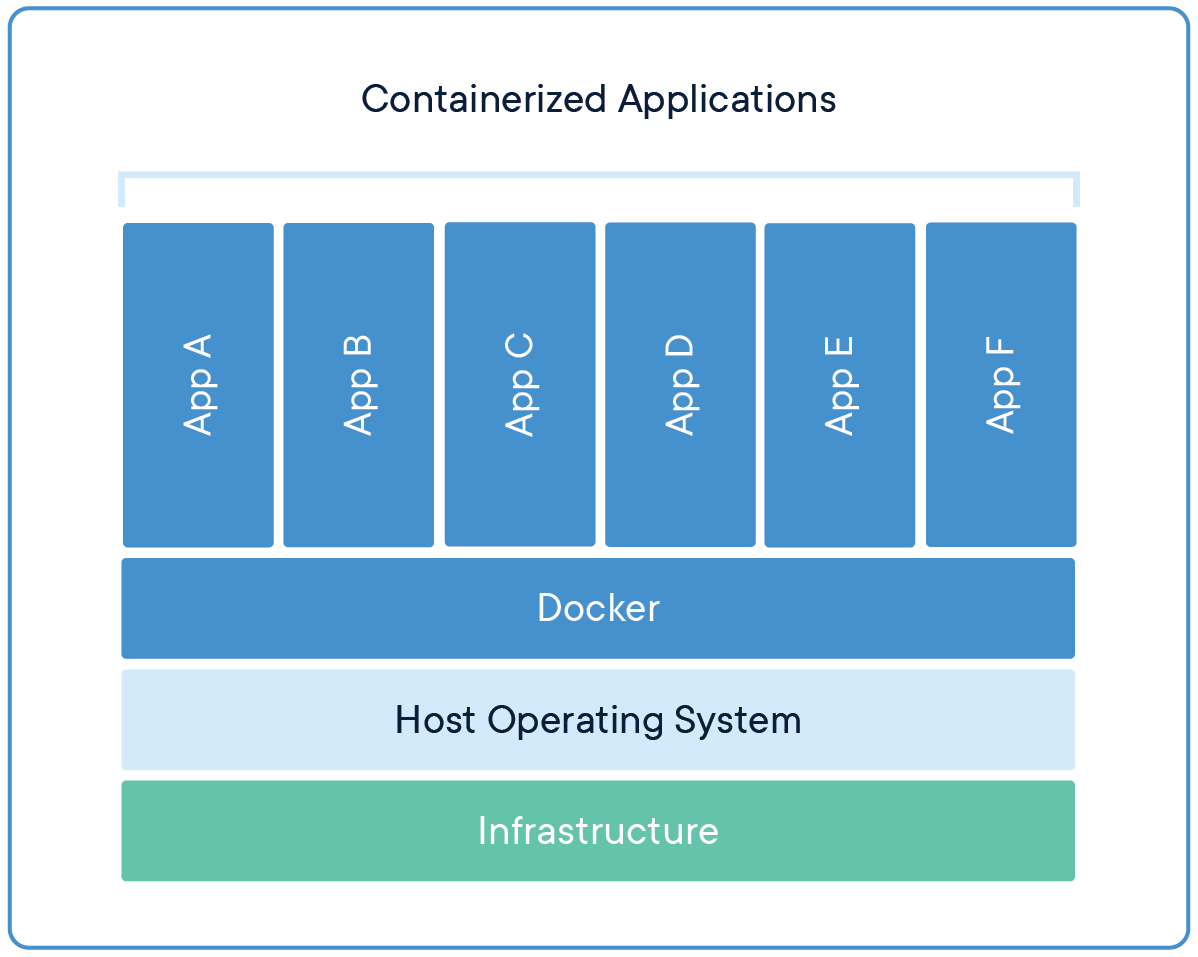
\includegraphics[width=0.45\textwidth]{img/grundlagen/technisch/docker_container}}\hspace{1cm}
	\subfigure[Virtuelle Maschine]{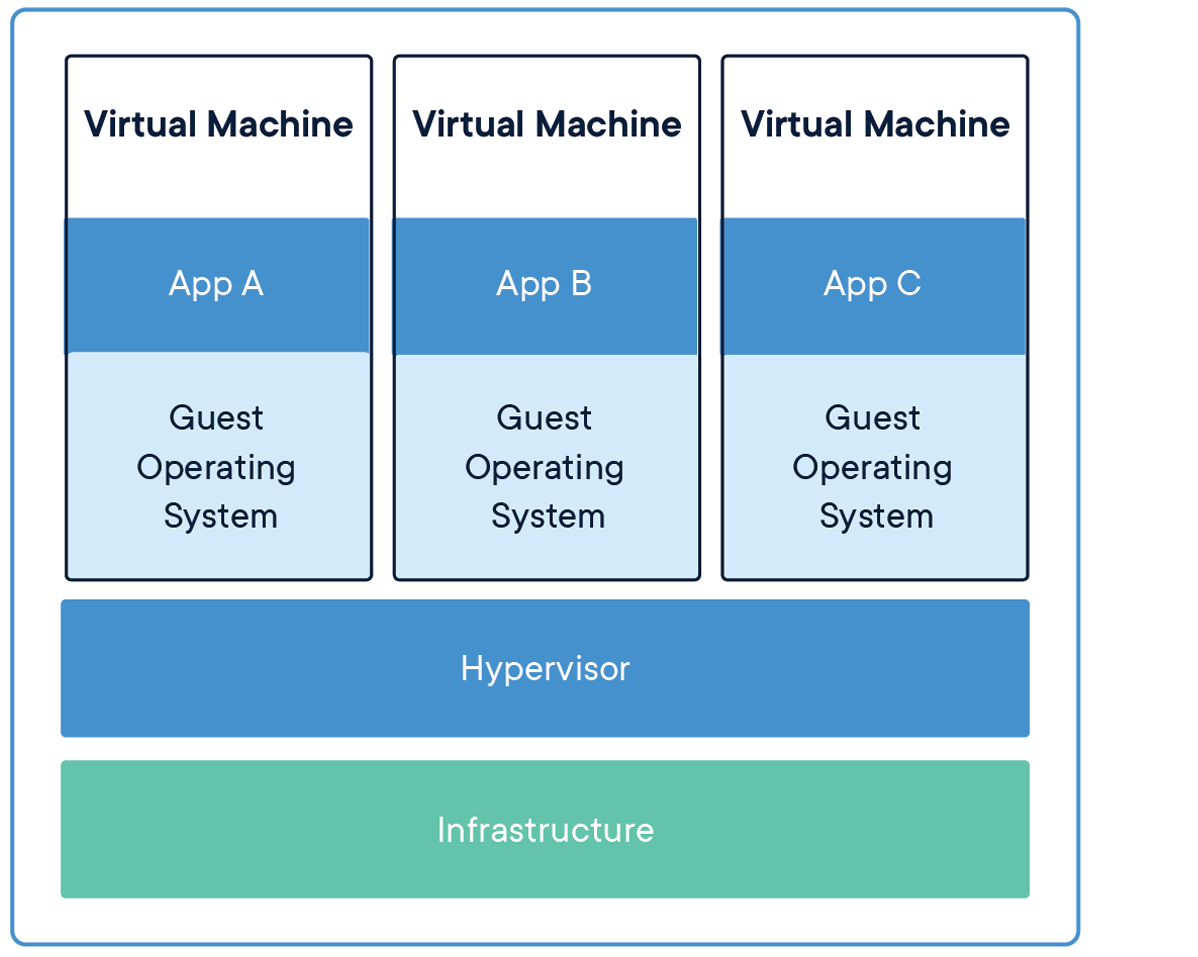
\includegraphics[width=0.45\textwidth]{img/grundlagen/technisch/docker_hypervisor}}
	\caption[Vergleich Container-Virtualisierung vs. virtuelle Maschine]{\label{fig:docker_container}Vergleich Container-Virtualisierung vs. virtuelle Maschine, \\Quelle: \cite{MS-DockerInc..05.03.2019}}
\end{figure}

Abbildung \ref{fig:docker_container} visualisiert die Architektur einer Container-Virtualisierung und zeigt einen Vergleich zur Hardware-Virtualisierung.\autocite[Vgl.][]{MS-ChrissiKraus.27.07.2018}$^,$\autocite[Vgl.][]{MS-MicrosoftCorporation.31.08.2018} 
Wie zu sehen ist, setzt Docker auf dem zugrunde liegenden Betriebssystem auf, wohingegen eine virtuelle Maschine als Gast-System agiert. 
Dabei verwaltet und verteilt bei virtuellen Maschinen ein Hypervisor die Ressourcen, welche die Betriebssysteme zur Verfügung gestellt bekommen. 
Ein Hypervisor ist also ein Manager für virtuelle Maschinen\autocite[Vgl.][]{MS-ReneBust.06.04.2010}. 
Docker-Container bekommen hingegen ihrere Ressourcen vom zugrundeliegenden Betriebssystem bereitgestellt.

Vorteile von Docker sind zum einen das hohe Maß an Integration und zum anderen eine gute Skalierbarkeit von Anwendungen. 
Dabei können die Docker-Container sehr einfach erzeugt, gestartet und gestoppt. 
Als Kern- und Steuerprogramm von Docker fungiert die sogenannte Docker-Engine. 
Sie ist neben dem Starten und Stoppen in der Lage vorhandene Container zu replizieren bzw. die Anzahl an Containern für einen speziellen Dienst bei Bedarf beliebig zu erhöhen oder zu verringern.
Hierzu kommt das Nebenprodukt Docker-Compose zum Einsatz. 
Dieses Werkzeug dient dem Erzeugen von Multi-Container-Anwendungen.
Der Integrationsaspekt entsteht dadurch, dass Docker mit anderer Software interagieren bzw. sich von dieser steuern lassen kann.\autocite[Vgl.][]{MS-Docker-Compose} 
% !TEX root =  ../../../master.tex
\subsection{Microservice}
\label{sec:grundlagen:microservices}

Für die Umsetzung von verteilten Systemen bzw. von Cloud-basierten Anwendungen hat sich in den letzten Jahren die Microservice-Architektur immer weiter etabliert.\autocite[Vgl.][Kapitel \enquote{Monolithic architecture overview}]{MS-Sharma.2016}
Die Verwendung dieser Architektur ist jedoch nicht neu, sondern wird bereits seit über zehn Jahren vom Unternehmen Amazon genutzt.\autocite[Vgl.][]{MS-Wolff.02.11.2015}
Die ursprüngliche Idee von Microservices wurde dabei aus dem Ansatz der \enquote{\textit{\ac{SOA}}} hergeleitet.\autocite[Vgl.][S. 1]{MS-Bucchiarone.2018}
Dabei gibt es für den Begriff Microservice keine konkrete Definition.\autocite[Vgl.][S. 3]{MS-Wolff.2018}
Vielmehr wird die Microservice-Architektur als Gegenteil der monolithischen Architektur verstanden, bei der die Software einem einzigen lauffähigen Baustein gleicht.
Dabei umfasst dieser Baustein alle Funktionen der Software, arbeitet autark und wird meist von mehreren Entwicklungsteams gleichzeitig entwickelt.
Dementsprechend ist eine lose Kopplung von einzelnen Bestandteilen nicht möglich.
Bei der Microservice-Architektur hingegen besteht die gesamte Software aus unabhängigen Komponenten, die jeweils von kleinen Teams entwickelt und bereitgestellt werden.\autocite[Vgl.][]{MS-Fowler.25.03.2014}
Jeder Microservice erfüllt in der Regel dabei nur eine Aufgabe, wie beispielsweise das Bereitstellen einer einzelnen \ac{REST}-Ressource.

% !TEX root =  ../../../master.tex
\subsection{PostgreSQL}
\label{ssec:PostgreSQL}

\enquote{PostgreSQL}, kurz Postgres, ist ein unter der PostgreSQL-Lizenz\autocite{rf-psqllicense} veröffentlichtes \ac{ORDBMS}, was es zu einem Open-Source-Projekt macht.\footnote{\url{https://www.postgresql.org/}}
Aktuell liegt das Projekt in der Version 12.3 vor.\footnote{\url{https://www.postgresql.org/docs/12/release-12-3.html}}
Das \ac{ORDBMS} verwendet die Datenbanksprache \ac{SQL} zur Ausführung der vom Benutzer angegebenen \ac*{CRUD}-Befehlen.
Dabei setzt Postgres auf ein umfangreiches Transaktionskonzept, welches auch besondere Verfahren, wie die \ac*{MVCC} zur effizienten Verarbeitung konkurrierender Zugriffe auf die Datenbank, beinhaltet.
Unter anderem durch dieses Transaktionskonzept ist PostgreSQL vollständig \ac*{ACID}-konform.\autocite[Vgl.][]{rf-psqlfeatures}

Neben den allgemeinen Funktionalitäten, die durch den \ac{SQL}-Standard vorgegeben sind, verwendet PostgreSQL auch eigene spezifische Verbesserungen und Weiterentwicklungen des Standards.
Zudem bietet PostgreSQL ein breites Angebot an selbst- sowie aufgrund der Strutkur als Open-Source-Projekt fremderstellten Erweiterungen.
Zur Benutzung bietet PostgreSQL einerseits nativ ein Kommandozeileninterface mit dem Namen \emph{PSQL} sowie andererseits ein graphisches Interface zur Verwaltung des \ac{ORDBMS} mit dem Namen \emph{pgAdmin}.
Postgres wird in der Regel als Bestandteil des Servers im Client-Server-Modell eingesetzt (vgl. Kapitel \myRefGeneral{ssec:Architektur}).

Ein großer Vorteil von Postgres ist das Erstellen von sogenannten \emph{Views}.
Über diese können dem Benutzer besondere Sichten, insbesondere wenn diese mehrfach verwendet werden, zur Verfügung gestellt werden.
Zudem können auf diesen weitere Berechnungen durchgeführt werden.
Beim Einfügen von Tupeln können Validierungen durchgeführt werden, \zb ob ein Wert zwischen 0 und 5 liegt.
Über eine Restriktion \engl{constraint} können Attribute einzigartig (\emph{unique}) sein.
Dies hilft \ua dann, wenn sich Benutzer bei einer Anwendung registrieren und sich einen Benutzernamen auswählen sollen, der nicht doppelt belegt werden darf.

Die zu Beginn erwähnte Lizenz von Postgres ist der MIT-Lizenz und der BSD-Lizenz ähnlich und erlaubt daher nicht nur die Nutzung, sondern auch das Kopieren, Erweitern und Verteilen der Software oder der Dokumentation dieser für jegliche Zwecke.
Diese Verwendungszwecke unterliegen keinerlei Auflagen und erfordern ebenfalls keinerlei Abgaben von Gebühren, weshalb das \ac{ORDBMS} sich für die Nutzung in diesem Projekt sehr gut eignet.\autocite[Vgl.][]{rf-psqllicense}

% !TEX root =  ../technisch.tex
\subsection{React}
\label{ssec:React}

Das Front-End beschreibt die Darstellung einer Webseite im Browser.
Die wohl bekannteste Sprache, um eine Webseite zu erstellen, ist \acs{HTML} in Verbindung mit \acs{CSS}.
\acs{HTML} beschreibt dabei den Aufbau der Webseite und in \acs{CSS} legt das Aussehen fest.
Um die Übersichtlichkeit im \acs{HTML}-Quelltext zu erhöhen, wird der \acs{CSS}-Quelltext in ein eigene Datei ausgelagert.

Eine heutige Front-End-Entwicklung findet häufig mit sogenannten Frameworks oder Bibliotheken statt.
Diese basieren in der Regel auf \acs{HTML} und \ac{JS}.
Der Unterschied zwischen einem Framework und einer Bibliothek lässt sich wie folgt erklären:
Ein Framework besteht aus mehreren Bibliotheken, wohingegen eine Bibliothek eine Sammlung von Klassen und Funktionen darstellt.\autocite[Vgl.][]{Libary_vs_Framework}
Der Informatiker Ralph Johnson beschreibt ein Framework folgendermaßen:
%
\begin{quote}
	\enquote{Das Framework stellt eine wiederverwendbare, gemeinsame Struktur für Anwendungen zur Verfügung. Entwickler binden das Framework in ihre eigenen Anwendungen ein und erweitern es so, dass es ihre bestimmten Anforderungen erfüllt.}
	\begin{center}{\textit{Ralph Johnson gemeinsam mit Brian Foote}}\end{center}
\end{quote}
%

Das \ac{DOM} bildet die Schnittstelle zwischen \acs{HTML} und \ac{JS}.
Alle \acs{HTML}-Elemente werden in Objekte umgewandelt.
D.~h., dass der Browser nie mit dem eigentlichen \acs{HTML}-Code arbeitet, sondern mit umgewandelten \ac{DOM}-Objekten.
Jeder \emph{Tag}, der in \ac{HTML} geschrieben wird, wird im \ac{DOM} als Objekt dargestellt.
Alle Objekte sind in einer Baumstruktur angeordnet.
Dies wird als Eltern-Kind-Prinzip bezeichnet.
Dies kann anhand der \acs{HTML}-Struktur in Quelltext~\vref{lst:ParentAndChild} erkannt werden.
Das Head- und Body-Objekt sind Kind-Objekte vom \acs{HTML}-Objekt.
Jedes Eltern-Objekt kann mehrere Kind-Objekte haben und diese können wiederum weitere Kind-Objekte besitzen.
\begin{lstlisting}[caption={Eltern-Kind-Prinzip},label={lst:ParentAndChild},language=HTML, showstringspaces={false}]
<!DOCTYPE html>
 <html> <!-- Eltern -->
   <head> <!-- Kind -->
    <title>Demo Eltern und Kind Prinzip</title> <!-- Kindes-Kind -->
   </head>
   <body> <!-- Kind -->
    code here
   </body>
 </html>
\end{lstlisting}

% https://books.google.de/books?id=2zrCDwAAQBAJ&printsec=frontcover&dq=react+hartmann&hl=de&sa=X&ved=0ahUKEwirn-u66uDpAhVExKYKHefEAPsQ6AEIKjAA#v=onepage&q=react%20hartmann&f=false 
React\footnote{\url{https://reactjs.org}} ist ein solches Framework.
Es ist eine Open-Source-JavaScript-Bibliothek mit deren Hilfe sogenannte \ac{SPA} erstellt werden.\autocite[Vgl.][]{hartmann2019react}
Das Hauptaugenmerk von React liegt auf dem komponentenbasierten Aufbau.
Eine Komponente stellt den Zustand der \ac{SPA} dar.
Sie repräsentiert einen fachlichen Teil wie \zb ein \enquote{einfaches} Eingabefeld \jinline|(Input)| oder auch komplexere Komponenten wie ein Formular.
Durch den komponentenbasierten Aufbau kann React nicht nur für die Entwicklung von Webanwendungen, sondern auch von \emph{iOS}- oder \emph{Android}-Apps verwendet werden.
Quelltext~\vref{lst:ReactKomponente} stellt eine Begrüßungs-Komponente dar, die einen Namen als Parameter \jinline|(props)| übergeben bekommt.

\begin{lstlisting}[caption={React-Komponente: Greeting},label={lst:ReactKomponente},language=HTML, showstringspaces={false}]
	import React from 'React'
	
	export const greeting = (name) => {
		return <h3>Hello {name}</h3>
	}
\end{lstlisting}

Um dieses Beispiel vereinfacht darzustellen, wird hierzu nachfolgend auf mehrere Studenten Bezug genommen.
Diese Studenten unterscheiden sich \zb in Vorname, Nachname, Alter und Matrikelnummer.
In React gibt es dementsprechend eine Komponente \jinline|Student|, welche die oben genannten Attribute als Parameter erhält.
Somit kann über einen allgemeinen Studenten ein spezifischer Studenten bekommen werden.

Dieses Vorgehen wird bei React als \emph{deklarative Komponente} bezeichnet und deshalb oft auch unter dem Begriff \texttt{UI as a Function} wiederzufinden.\autocite[Vgl.][]{hartmann2019react}
Wird eine Komponente in der \acs{SPA} geladen, wird das \acs{DOM} angepasst.
Hierbei werden nur die tatsächlichen Änderungen vorgenommen und nicht die komplette Seite geladen. \newline
Komponenten können einen internen Zustand haben \jinline|state| oder über externe Zustände \jinline|(properties)| verändert werden.
So kann \zb eine Komponente Account einen \jinline|state| besitzen.

Wie in Quelltext~\vref{lst:ReactKomponente} zu erkennen ist, hat die Komponente im Return-Statement einen Platzhalter \jinline|{ }|.
Diese ist ein typische React-Syntax.
In der Regel haben diese Komponenten die Dateiendung \acs{JSX}.
Sie wird bei der Verwendung von React empfohlen.
\acs{JSX} ist eine Erweiterung der JavaScript-\emph{Grammatik} und sorgt dafür, die interne Struktur zu ordnen und später in \acs{HTML} darzustellen.\autocite[Vgl.][]{WasIstJSX}

Ein Feature von React ist das Erstellen sogenannter \acp{PWA}.
\aclp{PWA} sind Webanwendungen, die vergleichbar mit nativen Apps auf dem Smartphone \enquote{installiert} werden können.
Es lässt sich eine Verknüpfung auf dem \emph{Homescreen} erstellen, sodass die \acs{PWA} wie eine normale App geöffnet werden kann.
Dadurch erhält der Nutzer den Eindruck einer native Anwendung aus dem Appstore des Geräteherstellers.
Solch eine \ac{PWA} kann offlinefähig sein, sodass sie auch verwendet werden kann, wenn der Benutzer keine Internetverbindung hat. \autocite[Vgl.][]{hartmann2019react}


\chapter{Anforderungsanalyse}
\label{c:analyse}
% !TEX root =  ../../master.tex
\section{Ist-Analyse}
\label{sec:IstAnalyse}

Bevor die Anforderungen an die Anwendung formuliert wurden, wurde die vorhergehende Umsetzung einer Learning-Analytics-Software analysiert.

Hierbei konnte zum einen ermittelt werden, dass die Seite via Google Firebase umgesetzt und zur Verfügung gestellt wurde.
Dabei ist jedoch festzuhalten, dass der vorhandene Code einen sehr niedrigen Umfang hatte, sowie unsauber war.
Dadurch wurde eine Weiterentwicklung oder eine Umsetzung, die auf dem vorangegangenen Projekt aufbaut, deutlich erschwert.

Hinzu kommt, dass die Visualisierung sehr generisch war und keine individuellen Anpassungen an die Gegebenheiten aufwies. Wodurch diese ebenfalls nicht weiter verwendet werden konnte.

Die erstellten und aufrufbaren Seiten boten keinerlei Funktionalitäten, da sämtliche Eingaben nicht persistent gespeichert, sondern bei dem nächsten Start der Anwendung überschrieben wurden.
Dies hat zur Folge, dass kein Bestandteil der vorherrschenden Anwendung für die Umsetzung der neuen Applikation verwendet werden konnte.
Somit mussten für diese Anwendung vollständig neue Anforderungen formuliert, sowie sämtliche Entwicklungsschritte wie beispielsweise die Konzeption und Verwirklichung vollständig neu begonnen werden.

% !TEX root =  ../../master.tex
\section{Anforderungen}
\label{sec:Anforderungen}

Die Anforderungen an das zu entwerfende und entwickelnde System lassen sich in mehrere Bereiche aufteilen.

Die Anwendung soll unabhängig vom Gerät des Endnutzers funktionieren.
So soll ein Student mit seinem mobilen Endgerät eine Umfrage ausfüllen können, während etwa ein Dozent die Umfrage am Desktop-Computer erstellt.
Daraus ergibt sich Anforderung [A1], die endgeräteunabhängige Nutzung der Anwendung.

Die Registrierung neuer Nutzer soll geschützt werden, um eine zu hohe Auslastung des Systems bzw. Angriffe zu verhindern.
Zudem sollen bereits registrierte und explizit dazu berechtigte Nutzer neue Konten anlegen können.
Somit ergibt sich Anforderungen [A2] und [A3], die Verwendung eines Registrierungsschlüssels bei der eigenen Registrierung sowie die Möglichkeit Nutzer durch bestehende Nutzer anzulegen.

Manuell angelegte Nutzer sollen bei ihrer ersten Anmeldung ein neues Passwort setzen müssen, um eine erhöhte Sicherheit zu gewährleisten.
Ebenfalls sollten Nutzer, deren Passwörter zurückgesetzt wurden, diese erneut setzen müssen.
Dazu ist eine Passwortänderungsseite erforderlich, welche wiederum als Passwortänderung für normale Nutzer verwendet werden kann.
Dies stellen die Anforderungen [A4], die Möglichkeit zur Passwortänderung, [A5], die Pflicht der Passwortänderung bei manueller Registrierung, sowie [A6], die Pflicht zur Passwortänderung bei manuell zurückgesetzten Passwörtern, dar.

Angemeldete Nutzer sollen in der Lage sein, sowohl neue Umfragen zu erstellen als auch bereits selbst erstellte Umfragen zu verwalten.
Die Umfragen sollen dabei mehrere Fragetypen beinhalten können, welche sich aus offenen Fragen, Single-Choice-Fragen, Multiple-Choice-Fragen sowie skalierten Fragen zusammensetzen.
Daraus ergeben sich die Anforderungen [A7], der Erstellung von Umfragen, [A8], der Verwaltung dieser, sowie [A9] der Verwendung verschiedener Fragetypen.

Erstellte Umfragen sollen dabei nicht automatisiert veröffentlicht werden, sondern nur auf Anfrage des Nutzers.
Dadurch soll es Dozenten möglich sein, Umfragen in Ruhe im Voraus vorzubereiten.
Diese unveröffentlichten Umfragen sollen zudem bearbeitbar sein, sodass vorher erkannte Fehler ausgebessert werden können.
Nach der Veröffentlichung sollen Umfragen wiederholt werden können.
Die Wiederholung soll dabei für mehrere Zeiträume, mehrere Kurse sowie mehrere Vorlesungen erfolgen können.
Die Ergebnisse der angelegten Umfragen sollen grafisch einsehbar sein.
Dies ergibt die Anforderungen [A10], die manuelle Veröffentlichung der Umfrage, [A11], die Bearbeitbarkeit unveröffentlichter Umfragen, [A12], die Wiederholbarkeit der Umfragen, und [A13], der grafischen Darstellung der Umfrageergebnisse.

Die Teilnahme an Umfragen soll anonym erfolgen und für die Teilnehmer so simpel wie möglich sein.
Dies stellt die letzten funktionalen Anforderungen [A14], die anonyme Teilnahme an Umfragen, sowie [A15], der Möglichkeit zur einfachen Teilnahme, dar.

Da die Anwendung im Rahmen eines Projektes der \acs{DHBW} Mannheim konzeptioniert wird, ist das Farbschema dieser an das Corporate Design der \acs{DHBW} Mannheim anzupassen.
Dies ist die einzige nicht-funktionale Anforderung [A16], Farbschema im Corporate Design.

In Tabelle~\vref{tab:Anforderungen} sind alle Anforderungen noch einmal übersichtlich aufgelistet.
Dabei erfolgt eine Kennzeichnung, ob es sich um eine funktionale (f) oder nicht-funktionale (nf) Anforderung handelt.
Während funktionale Anforderungen definieren, \emph{was} die Software umsetzen soll, geben nicht-funktionale Anforderungen die Leistungs- und Qualitätsanforderungen sowie Rahmenbedingungen wieder.\autocite[Vgl.][S. 10]{nl-robertson2012mastering}\autocite[Vgl.][S. 3 ff]{nl-braun2016nicht}

\begin{table}
  \setlength\extrarowheight{3pt}
\centering
  \begin{tabular}{|C{1cm}|C{1cm}|L{12cm}|}
    \hline
    \textbf{Nr.} & \textbf{Art} & \textbf{Beschreibung} \\
    \hline
    {\label{Anf:A1}A1} & f & Endgeräteunabhängige Nutzung \\
    \hline
    {\label{Anf:A2}A2} & f & Registrieren mit Registrierungsschlüssel \\
    \hline
    {\label{Anf:A3}A3} & f & Manuelles Registrieren neuer Nutzer \\
    \hline
    {\label{Anf:A4}A4} & f & Möglichkeit zur Passwortänderung \\
    \hline
    {\label{Anf:A5}A5} & f & Pflicht zur Passwortänderung bei manueller Registrierung \\
    \hline
    {\label{Anf:A6}A6} & f & Pflicht zur Passwortänderung bei zurückgesetztem Passwort \\
    \hline
    {\label{Anf:A7}A7} & f & Erstellen von Umfragen \\
    \hline
    {\label{Anf:A8}A8} & f & Verwalten von Umfragen \\
    \hline
    {\label{Anf:A9}A9} & f & Verwendung verschiedener Fragetypen \\
    \hline
    {\label{Anf:A10}A10} & f & Manuelle Veröffentlichung der Umfragen \\
    \hline
    {\label{Anf:A11}A11} & f & Bearbeitbarkeit unveröffentlichter Umfragen \\
    \hline
    {\label{Anf:A12}A12} & f & Wiederholbarkeit von Umfragen \\
    \hline
    {\label{Anf:A13}A13} & f & Grafische Darstellung der Umfrageergebnisse \\
    \hline
    {\label{Anf:A14}A14} & f & Anonyme Teilnahme an Umfragen \\
    \hline
    {\label{Anf:A15}A15} & f & Möglichkeit zur einfachen Teilnahme an Umfragen \\
    \hline
    {\label{Anf:A16}A16} & nf & Farbschema im Corporate Design \\
    \hline
  \end{tabular}
  \caption{Übersicht der Anforderungen}
  \label{tab:Anforderungen}
\end{table}

% !TEX root =  ../../master.tex
\section{Abgrenzung zu Alternativen}
\label{sec:AbgrenzungZuAlternativen}

Im folgenden Abschnitt soll die Anwendung von verschiedenen Alternativen abgegrenzt werden.
Dabei soll hervorgehoben werden, worin sich das zu entwickelnde Umfrage-Tool von diesen Alternativen unterscheidet.

Zunächst soll Bezug auf die bekannte Lernplattform Moodle genommen werden.
Moodle bietet die Möglichkeit Kurse, individuelle Dashboards und Kalender anzulegen.\autocite[Vgl.][]{ms-moodle-features}.
Moodle bietet zunächst offiziell eine Möglichkeit Umfragen zu erstellen, jedoch ist dies durch die verwendeten Einstellungen in der Moodle-Version der \acs{DHBW} Mannheim nicht möglich.\footnote{Laut Aussagen der Betreuerin dieser Arbeit}
Außerdem können diese Umfragen in der Regel nicht an externe, Nicht-Moodle-Nutzer weitergegeben werden.
Genau diese Spezialisierung soll die Software dieses Projektes von Moodle unterscheiden bzw. hervorheben.
Dabei ist besonders entscheidend, dass die Software die wiederholte Nutzung von Umfragen ermöglichen soll.

Neben Moodle gibt es eine Vielzahl von Umfrage-Tools, die zur Erstellung von internen und externen Umfragen genutzt werden können.
Bei diesen ist es jedoch oftmals nicht möglich Vorlagen für Umfragen zu erstellen, sodass Umfragen mehrmals gestellt werden können.
Weiterhin ist die \acs{DHBW} Mannheim an Auflagen gebunden, wie sie Daten erheben darf.
Beispielsweise muss bei einer Datenerhebung darauf geachtet werden, dass der Datenschutz eingehalten und die Anonymität der Teilnehmer gewahrt wird.
Dementsprechend ist eine umfangreiche vorherige Prüfung eines Umfragetools oftmals nicht vermeidbar, um eventuelle Tracking-Funktionen oder ähnliches zu entdecken.
Außerdem hat die \acs{DHBW} Mannheim keinen Einfluss auf potenzielle Änderungen solcher Tools und befindet sich hier in einer entsprechenden Abhängigkeit, die ein Risiko darstellt.
Weiterhin sind professionelle Umfrage-Tools, die gegebenfalls alle nötigen Vorraussetzungen mit sich bringen, entsprechend kostenintensiv.

Aus diesen Gründen ist es für die \acs{DHBW} Mannheim von Nutzen, ein eigenes Umfrage-Tool zu besitzen.
Dieses Tool kann entsprechend an die Bedürfnisse der \acs{DHBW} angepasst werden.


\chapter{Konzeption}
\label{c:konzeption}
% !TEX root =  ../../master.tex
\section{Gesamtkonzept}
% !TEX root =  ../gesamtkonzept.tex
\section{Grundlegende Architektur}
\label{sec:Architektur}

Das neue System setzt, wie \citeauthor{MS-Fielding.} empfiehlt, auf das Client-Server-Modell. 
Dabei soll ein mehrfacher und voneinander unabhängiger Zugriff sowie die Entwicklung von Erweiterungen oder die Integration in bereits bestehende Systeme ermöglicht werden.
Dies soll die Umsetzung der Anforderung \hyperref[Anf:A1]{A1} erleichtern.
Der Server, wie in Abbildung \ref{img:einkaufBPMN} zu erkennen, eine \ac{API} für den Client zur Verfügung, um auf die Geschäftslogik und somit alle Ressourcen zugreifen zu können.
Der Client ist somit lediglich für die Darstellung verantwortlich und übernimmt nur geringfügige Überprüfungen der Eingaben des Nutzers, sodass bei absehbar falschen Anfragen der Server nicht ausgelastet wird.
Zur Darstellung stellt der Client dabei die Visualisierungsmethoden zur Verfügung und arbeitet die von der Schnittstelle erhaltenen Daten auf.

\begin{figure}[h]
  \centering
  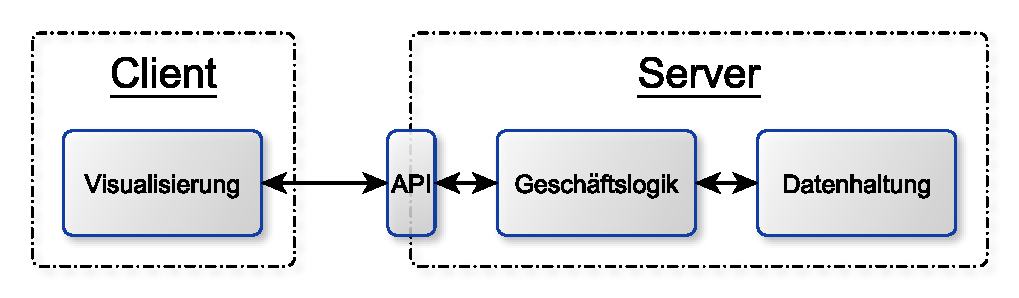
\includegraphics[width=0.75\textwidth]{img/konzeption/gesamtkonzept/Architektur.pdf}
  \captionsetup{format=plain,justification=centering}
  \caption[Architekturmodell]{Architekturmodell. \\Quelle: Eigene Darstellung.}
  \label{img:einkaufBPMN}
\end{figure}

Grundlegend ist deshalb die Architektur dem \ac{MVC}-Konzept nachempfunden, da der Server das Model durch die vorhandene Datenbank und die darin vorhandenen Relationen darstellt sowie die View des Konzepts durch den Client repräsentiert wird.
Der Controller wird dabei zu einem Teil durch die Geschäftslogik im Server und der damit verbundenen \ac{API} repräsentiert.
Zum anderen ist dieser jedoch ebenso im Client durch eine Sammlung und Aufarbeitung der Daten sowie einer geringfügigen Überprüfungen der Nutzereingaben vorhanden.\autocite{rf-leff2001web}
% !TEX root =  ../../master.tex
\section{Server}

\subsection{Grundlegender Aufbau}
Zur Implementierung der Geschäftslogik wird ein Webserver mit Node.js in Verbindung mit dem Framework Express entwickelt.
Bei Node.js handelt es sich um eine JavaScript-Laufzeitumgebung, die die serverseitige Entwicklung mit JavaScript ermöglicht und dabei auf der V8-JavaScript-Implementierung von Google aufsetzt.\autocite[Vgl.][]{nl-openjsfoundation2020nodejs}
Express ist ein Framework für Node.js, um Webanwendungen und \acsp{API} zu entwickeln und wegen der Einfachheit weit verbreitet.\autocite[Vgl.][]{nl-strongloop2017express}

Für die Datenhaltung wird PostgreSQL, ein \ac{RDBMS}, verwendet.
Wie bei allen \acsp{RDBMS} können Daten über die Sprache \acs{SQL} abgefragt und editiert werden.
Mithilfe eines entsprechenden Moduls kann sich innerhalb der Node.js-Anwendung mit der PostgreSQL-Datenbank verbunden werden, sodass \acs{SQL}-Befehle ausgeführt werden können.\autocite[Vgl.][]{nl-carlson2020nodepostgres}

Für jeden \acs{API}-Endpunkt wird jeweils eine Funktion aufgerufen, die die übergebenen Daten entgegennimmt, prüft und daraufhin auf die Datenbank zugreift.

\subsection{Zugriffskontrolle}
Die Zugriffskontrolle erfolgt im Back-End.
Da jegliche Kontrolle, die im Front-End implementiert ist, clientseitig ausgeführt wird, ist sie auch durch einen Angreifer ohne Weiteres aufzuheben und damit als unsicher anzusehen.
Nichtsdestotrotz sind natürlich auch im Front-End entsprechende Maßnahmen implementiert.
Diese dienen allerdings nicht dem Schutz gegen unbefugte Zugriffe, sondern sollen lediglich dafür sorgen, dass Nutzer bereits in der graphischen Darstellung erkennen, wozu sie berechtigt sind und worauf sie Zugriff haben.
Alles andere führt für Benutzer nur zu Verwirrung.

Für die tatsächliche Zugriffskontrolle im Back-End werden, wie bereits in der Konzeption in Abschnitt~\ref{sec:authentifizierung} erläutert, Passwörter beziehungsweise Session-IDs genutzt.
Bei der Registrierung oder einer Anmeldung wird eine solche Session-ID ausgestellt.
Bei jedem Zugriff auf einen der \acs{API}-Endpunkte wird, bevor überhaupt irgendeine Aktion ausgeführt wird, die Korrektheit dieser Session-ID geprüft.
Damit ist sichergestellt, dass eine entsprechende Prüfung nicht versehentlich beim Implementieren eines einzelnen \acs{API}-Endpunkts vergessen werden kann.
Diese entsprechende Funktion ist in Quelltext~\vref{implementation-server-auth-check} abgebildet.

\begin{lstlisting}[language=javascript, caption={Standardmäßige Authentifizierung}, label={lst:implementation-server-auth-check}]
exports.checkUserAuthorization = function (request, callback) {
	const { username, sessionId } = request.body;
	if (username === undefined || sessionId === undefined)
		return callback(false);
	db.query('SELECT * FROM users WHERE lower(username) = lower($1) AND session_id = $2;', [username, sessionId], (err, dbResult) => {
		if (err || dbResult.rows.length !== 1) {
			callback(false);
		} else if (dbResult.rows[0].password_change_required) {
			callback(false, "Error: Password change required");
		} else {
			callback(true);
		}
	});
};
\end{lstlisting}

So wird zunächst der Nutzername und die Session-ID ausgelesen.
Daraufhin kann nach einem entsprechenden Eintrag in der Datenbank gesucht werden.
Wird kein Ergebnis gefunden oder ist ein Passwortwechsel gefordert, so wird der Zugriff verwehrt.

Selbstverständlich gibt es auch \acs{API}-Endpunkte, auf die Zugriffe ohne Autorisierung möglich sein müssen.
Dies umfasst einerseits das Beantworten von Umfragen und andererseits das Registrieren, Passwortwechseln und Anmelden, bei dem Nutzer logischerweise noch keine gültige Session-ID besitzen, da sie diese ja dadurch erst erhalten wollen.
Entsprechende Ausnahmen sind über eine Whitelist gelöst, sie werden also explizit aufgelistet.
Auch hierbei steht im Vordergrund, dass \acs{API}-Endpunkte standardmäßig geschützt sind und nicht versehentlich Sicherheitslücken entstehen.

Darüber hinaus wird bei jeder Aktion die Berechtigung geprüft.
Bei der Bearbeitung eines \texttt{SurveyMasters} wird zum Beispiel zuerst einmal validiert, ob dieser auch dem angemeldeten Nutzer zugeordnet ist.

% !TEX root =  ../../master.tex
\section{Client}
\authorsection{\authorSG}

Wie bereits in Kap. \vref{ssec:React} beschrieben, wird in diesem Projekt React verwendet. 
Für die Unterteilung der verschiedenen Komponenten soll auf eine spezielle \acfp{UX} und \acfp{UI} gelegt werden. 
Im folgenden soll auf den Aufbau der Benutzeroberfläche eingegangen werden. 

\subsection{Participate}
Im Bezug auf Verwendbarkeit wie in Kap. \vref{sec:UserJourney} beschrieben ist die Startseite die \emph{Participate}-Seite. 
In dieser soll der Benutzer bzw. Student der an einer Umfrage teilnimmt, einen \emph{Surveycode} wie z.B. \emph{\texttt{OYZQGGXOF9}} eingeben, um an der Umfrage zu partizipieren. 

Anschließend wird der Benutzer auf die Umfrageseite weitergeleitet, auf der er die benötigten Felder ausfüllt (siehe \vref{ssec:Umfrage}).

\subsection{Umfrage}
\label{ssec:konzept:client:umfrage}
Wie in Abbildung~\vref{fig:MockUmfrageTeilnehmer} dargestellt, wird der Teilnehmer auf die zuvor angegebene Umfrage geleitet.
Die Fragen werden dabei jeweils in einer eigenen Karte dargestellt.
Durch Drücken eines Knopfes soll der Teilnehmer zur nächsten Frage gelangen.
Gleichzeitig soll dem Benutzer sein Fortschritt verdeutlicht werden, um die Dauer der Umfrage abschätzen zu können.
Die Abgabe der Umfrage erfolgt identisch zum Fragenwechsel.
Der Teilnehmer soll dabei Feedback erhalten, ob seine Teilnahme erfolgreich war.

Durch diesen Vorgang sollen die Anforderungen~\hyperref[Anf:A14]{A14}, die anonyme Teilnahme, sowie \hyperref[Anf:15]{A15}, die einfache Teilnahme an einer Umfrage, erfüllt werden.

\begin{figure}[H]
	\centering
	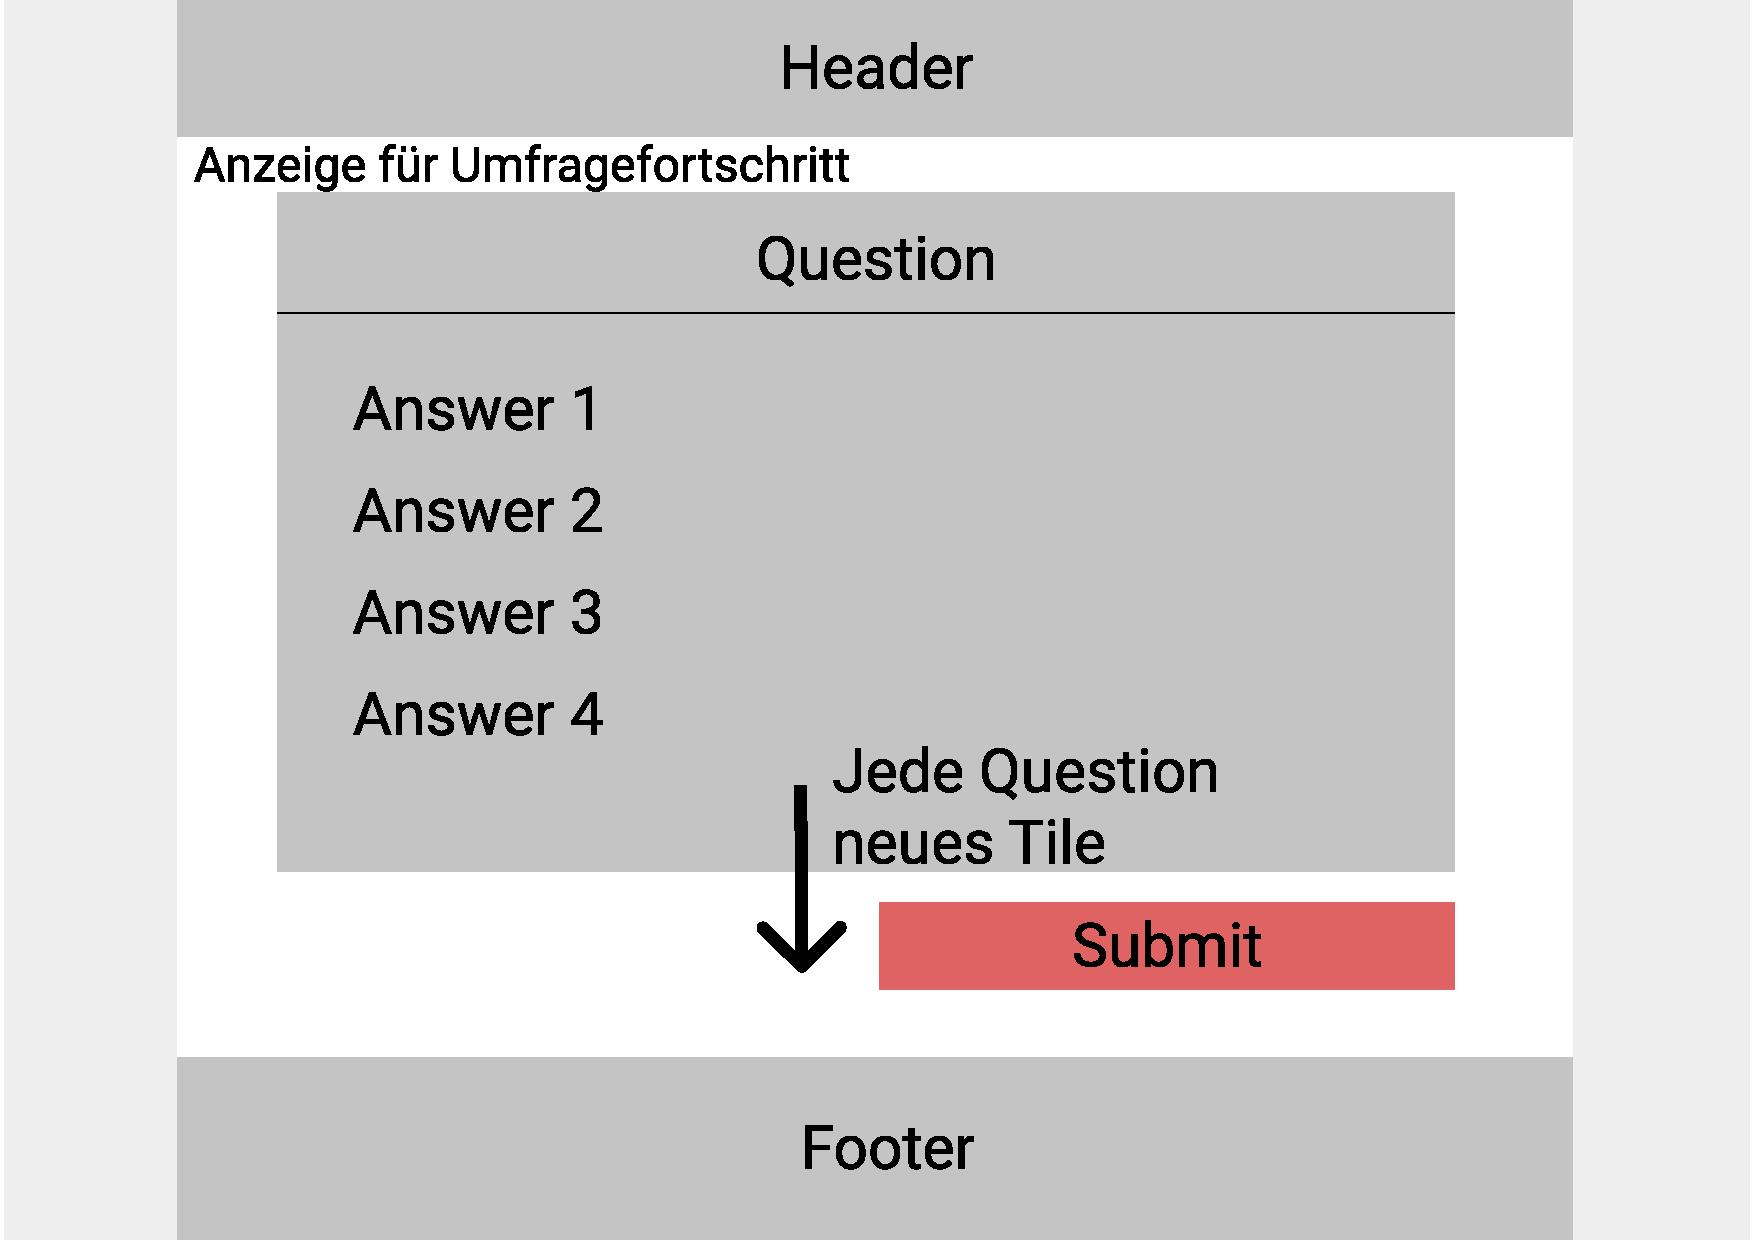
\includegraphics[width=0.7\textwidth]{img/konzeption/client/umfrage_teilnehmer}
	\captionsetup{justification=centering, format=plain}
	\caption[Mock-Up der Teilnahmeseite]{Mock-Up der Teilnahmeseite\\\figma}
	\label{fig:MockUmfrageTeilnehmer}
\end{figure}


\subsection{Result-Dashboard}
\label{ssec:ResultDashboard}





\subsection{Unterteilung der Gliederungsansichten}

\begin{itemize}
	\item Beschreibung der Mockups 
	 \begin{itemize}
		 \item Was haben wir uns bei den einzelnen Seiten gedacht
		 \item Wie sollten die Seiten grundsätzlich aussehen. (Brainstorming)
		 \item evtl. bissel auf Designthinking eingehen
		 \item Welches tool haben wir dazu genutzt
	 \end{itemize}
	 \item Recherche zu vorhandenen Umfragetools --> (https://www.polly.ai/slack-poll, https://strawpoll.de/, https://www.limesurvey.org/de/, https://www.surveymonkey.de/, https://pingo.coactum.de/)
	 --> Ideensammlung und Marktrecherche
	 \item Grundlegende Idee der Einfachheit (evtl Gesamtkonzept)
	 \item Man könnte auf den User Journey eingehen
	 \item Anlehnung an DHBW farben sind vorgesehen
	 \item Orientierung an modernen Websites mit header und footer
	 \item Hinblick auf mobile usage
\end{itemize}
\subsection{Bestimmung von Darstellungsformen}
% !TEX root =  master.tex
\section{Personas}
\label{sec:Personas}

% !TEX root =  master.tex
\subsection{Persona a}
% !TEX root =  master.tex
\newcommand{\ariane}{Ariane Aris\xspace}
% -------------------------------------------------------
% Studierende Person
%
% --------------------------------------------------------
\newpage
\cvsect{\ariane}
\begin{minipage}[t]{0.5\textwidth}
	\vspace{-3.6cm}
	\renewcommand{\arraystretch}{1.5}
	\begin{tabular}{l l}
		Name: & \ariane \\
		Alter: & 20 \\
		Tätigkeit: & Studentin der Wirtschaftsinformatik \\
		Skills: & 3/5 \hspace{-1cm} \begin{barchart}{5.0}
			\baritemNL{}{3}
		\end{barchart} \\
	\end{tabular}
\end{minipage}
\hfill
\begin{minipage}[t]{0.4\textwidth}
	\flushright
	\includegraphics[width=0.70\textwidth]{img/personas/ariane}
\end{minipage}
\autocite{rf-unsplash-studentin}

Das möchte ich gerne haben:
\begin{itemize}
	\item einfaches, schnelles und unkompliziertes Erstellen neuer Umfragen für ihre wissenschaftlichen Arbeiten
	\item Auswertung der Umfrageergebnisse
    \item Teilnahme an anderen Umfragen
\end{itemize}

Mit der zweiten Persona, \ariane, wird eine Studentin für Wirtschaftsinformatik einer Hochschule beschrieben.
\ariane nimmt primär die Rolle einer Umfrageerstellerin und sekundär die Rolle einer Teilnehmerin ein.
Dabei möchte sie sowohl einfach eine Umfrage erstellen, als auch bei anderen Umfragen teilnehmen können.
% !TEX root =  master.tex

% -------------------------------------------------------
% umfrageteilnehmende Person
% -------------------------------------------------------
\newpage
\cvsect{Julian Weigert}
\begin{minipage}[t]{0.5\textwidth} 	\vspace{0.2\baselineskip} % Required for vertically aligning minipages
	\begin{entrylist}
		\entry
		{Name:}
		{Julian Weigert}
			\entry
		{Alter:}
		{24}
		\entry
		{Tätigkeit:}
		{Student für BWL}
	\end{entrylist}
	\begin{barchart}{5.0}\hspace{-1mm}
		\baritem{Skills}{2}
	\end{barchart}
\end{minipage}
\hfil
\begin{minipage}[t]{0.4\textwidth} 	\vspace{0.0\baselineskip} % Required for vertically aligning minipages
	\flushright
	\includegraphics[width=0.70\textwidth]{img/personas/julian}
\end{minipage}
\autocite{rf-unsplash-student}

Das möchte ich gerne haben:
\begin{itemize}
	\item Umfragen anonym durchführen
    \item Umfragen auf seinem Smartphone durchführen
    \item Umfragen auch später durchführen
\end{itemize}

Mit der dritten Persona, Julian Weigert, wird ein technisch weniger begabter Student einer Hochschule beschrieben.
Julian Weigert nimmt primär die Rolle des Umfrageteilnehmers ein, wobei er die Umfragen gerne an seinem mobilen Endgeräten bearbeiten möchte.
Durch seinen eng getakteten Zeitplan möchte er Umfragen auch Tage nach der Herausgabe des Links beantworten können.


% !TEX root =  ../../master.tex
\section{User-Journey}
%\label{sec:user_journey}
%Anhand der nun weitestgehend geschilderten Anforderungen aller Personas wurde der Aufbau der Website für das entwickelte Kinobuchungssystem entschieden.
%Diese gewählte Struktur wird im Folgenden anhand eines Beispiels geschildert, in welchem ein Endnutzer drei Tickets für eine spezielle Filmvorführung bucht.
%Vorausgesetzt ist hierbei, dass der Nutzer tatsächlich eine Online-Buchung vornimmt und nicht direkt im Kino anruft, um ein Ticket zu erwerben bzw. einen Sitzplatz zu reservieren.
%
%\begin{figure}[ht]
%	\centering
%	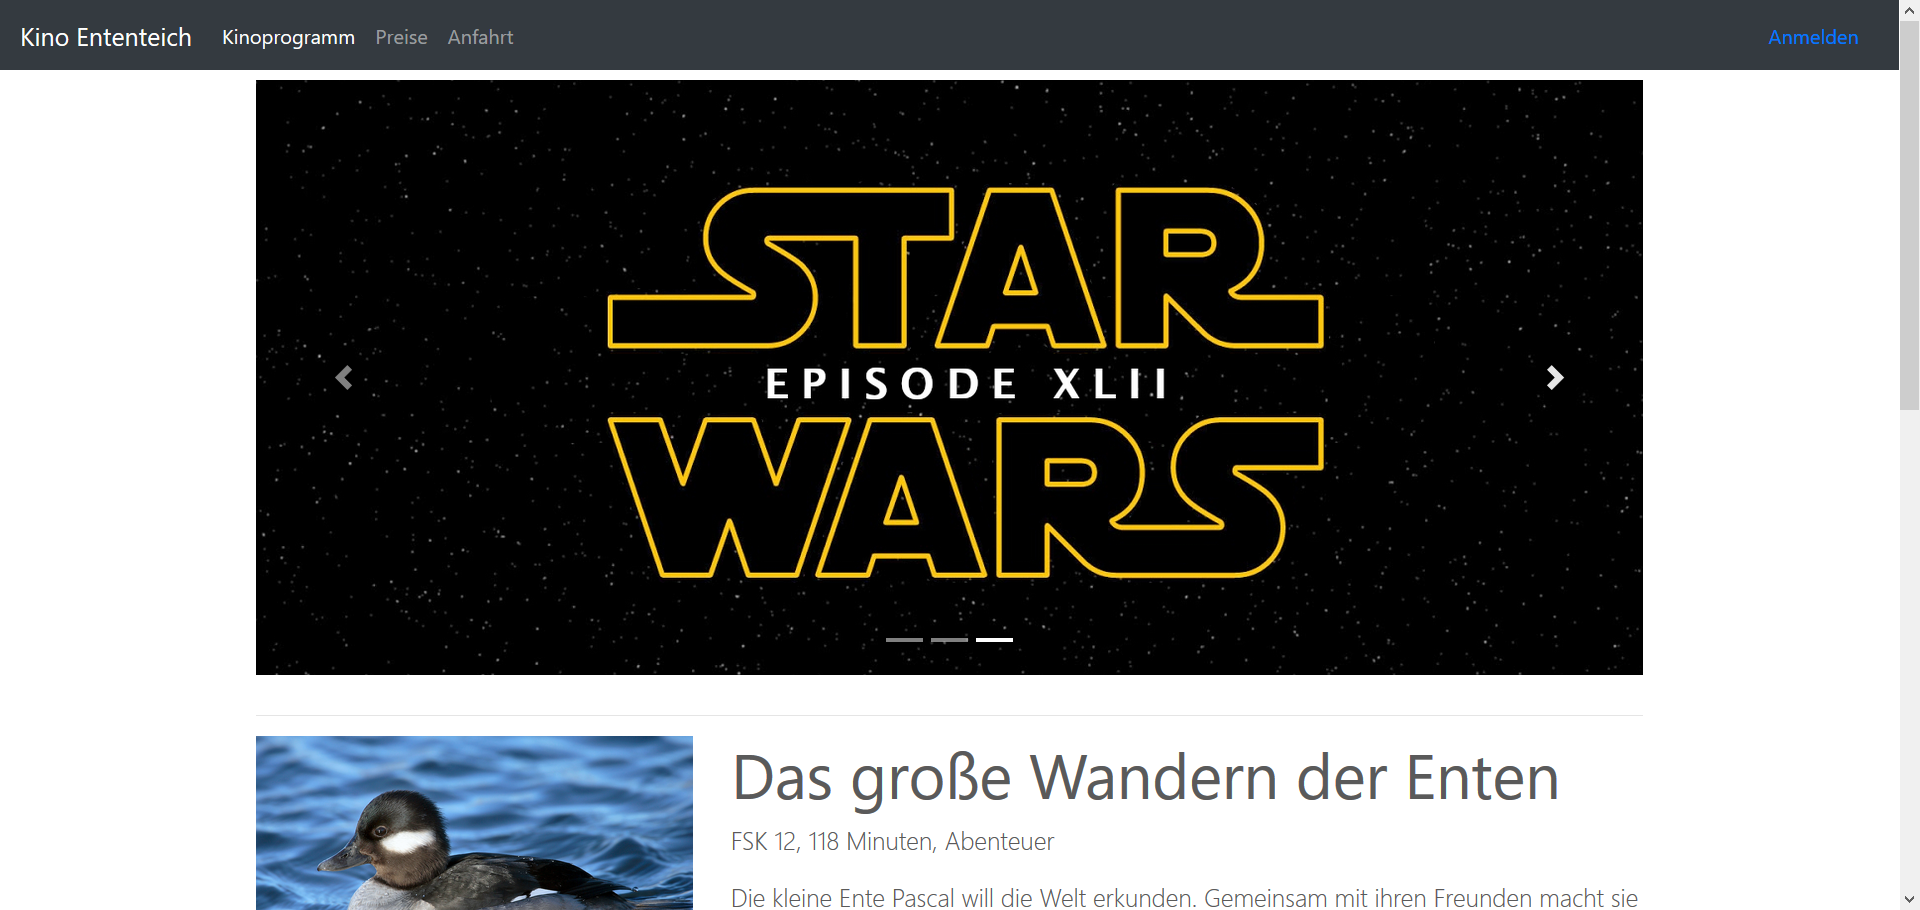
\includegraphics[width=\textwidth]{img/screenshots/startseite00}
%	\captionsetup{format=hang}
%	\caption{Startseite}
%	\label{fig:startseite00}
%\end{figure}
%
%Bei Aufruf der Startseite des Kinos wird dem Nutzer eine Übersicht über alle momentan im Kino laufenden Filme präsentiert.
%Ganz oben befindet sich dabei ein Karussell mit den beliebtesten Filmen.
%Darunter ist eine Liste mit allen Filmen.
%Durch Herauf- und Herabscrollen lässt sich schnell durch diese Liste navigieren, das Finden des gesuchten Films wird durch die großen Cover-Bilder neben dem Titel erleichtert.
%Durch Anwählen des Filmtitels wird der Nutzer auf die Seite für diesen Film geleitet, auf der alle Vorstellungen des Films innerhalb der nächsten Tage aufgelistet sind.
%Dort findet sich auch eine detaillierte Beschreibung und eine Bewertung des Films durch andere Benutzer (vgl. Anhang \vref{sec:screenshots_frontend}).
%
%Eine jede dieser Vorstellungen ist durch einen Knopf in der nach Tagen geordneten Tabelle repräsentiert, mit der passenden Uhrzeit als Beschriftung.
%Wurde der Knopf mit dem gewünschten Vorstellungszeitpunkts ausgewählt, so wird der Nutzer zur Sitzplatzübersicht und -auswahl weitergeleitet.
%
%Als nächstes ist für den Anwender die Wahl der Sitzplätze relevant.
%Dies geschieht im entwickelten Buchungssystem durch die Anwahl der Plätze in einer 2D-Grafik des Kinosaals, in welcher bereits belegte, freie und eigens angewählte Plätze farblich voneinander abgehoben sind.
%Nach der Auswahl der gewünschten Sitzplätze sollte der Nutzer nun in der Lage sein, die Preiskategorien der Plätze (Ermäßigungen usw.) auszuwählen und den Einzel- sowie Gesamtpreis der Auswahl einsehen zu können.
%
%\begin{figure}[ht]
%	\centering
%	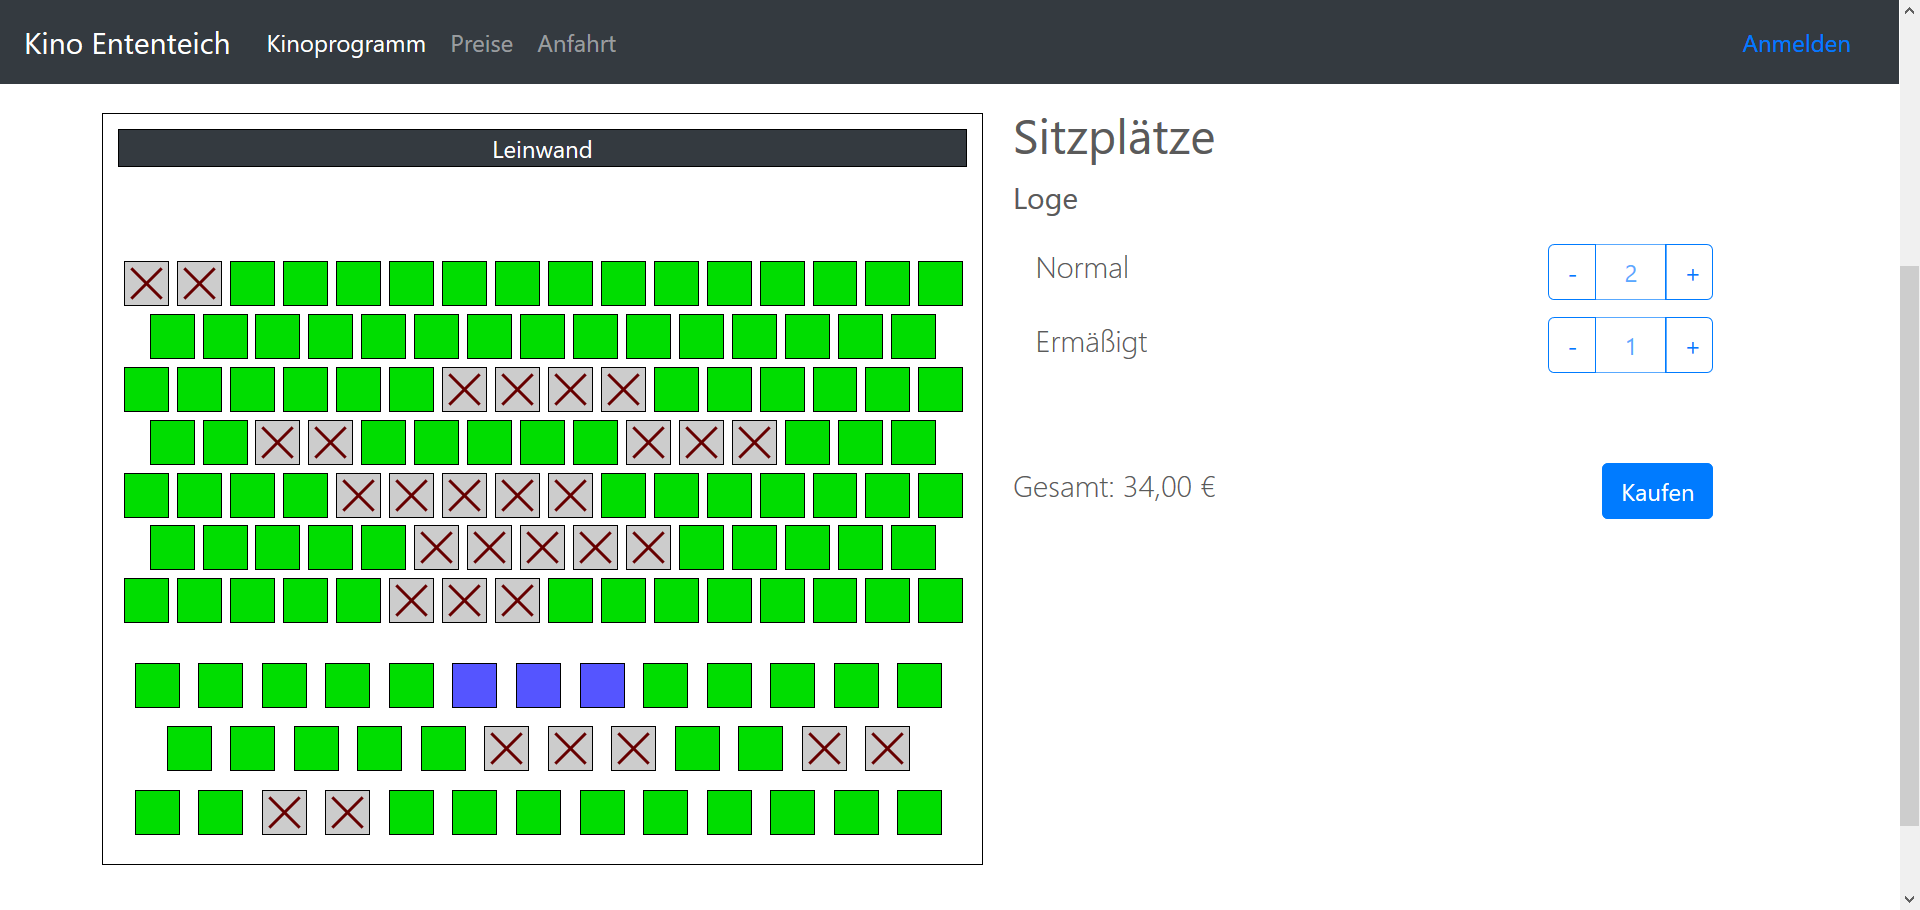
\includegraphics[width=\textwidth]{img/screenshots/vorstellung02}
%	\captionsetup{format=hang}
%	\caption{Auswahl der Sitzplätze}
%	\label{fig:vorstellung02-2}
%\end{figure}
%
%Ist der Nutzer mit diesem Schritt fertig, kommt es nun zum Bezahlvorgang für die ausgewählten Tickets.
%Hier soll der Nutzer eine kompakte Übersicht über die Bestellung erhalten, und nach Überprüfung seiner Auswahl seine persönlichen Daten (Vorname, Nachname und E-Mail-Adresse) angeben können.
%Drüber hinaus soll noch die Auswahl zwischen mehreren Zahlungsmethoden sowie die Eingabemöglichkeit für Rabattcodes angeboten werden.
%
%Mit der Zahlungsbestätigung ist der Nutzer im letzten Schritt des Buchungsvorgangs angelangt.
%Hier werden erneut die zusammengefassten Details der Bestellung (Kosten, Sitzplätze, Filmdetails und Vorstellungszeitpunkt) sowie ein Bestätigungstext angezeigt.
%Außerdem wird dem Nutzer sein digitales Ticket in Form eines \acs{QR-Code}s angezeigt, welches der Anwender auch per E-Mail zugesandt bekommt oder mithilfe eines Accounts in der mobilen App abrufen kann.
%Dieser Code enthält alle Infos über das Ticket und ist im Kino gleichwertig mit einer ausgedruckten Version.
%
%Neben diesem Anwendungsfall gibt es natürlich noch andere Berührungspunkte der Anwender mit dem System außerhalb der Aufgabenstellung dieser Arbeit.
%Hierzu zählen unter anderem eine Ticketbuchung bzw. -reservierung per Telefon sowie die Verarbeitung einer Buchung durch einen Kinomitarbeiter.
%Im Allgemeinen ähneln sich die Schritte insofern, dass Film-, Vorstellungs- und Sitzplatzauswahl vom Ablauf her gleich bleiben, für den Kinomitarbeiter jedoch kompakter dargestellt werden können.
%Filmbeschreibungen, Bewertungen, Titelbilder usw. spielen hier keine Rolle, da diese Informationen für den Mitarbeiter als Fachmann irrelevant sind.
% !TEX root =  ../../master.tex
\section{Server}

\subsection{Grundlegender Aufbau}
Zur Implementierung der Geschäftslogik wird ein Webserver mit Node.js in Verbindung mit dem Framework Express entwickelt.
Bei Node.js handelt es sich um eine JavaScript-Laufzeitumgebung, die die serverseitige Entwicklung mit JavaScript ermöglicht und dabei auf der V8-JavaScript-Implementierung von Google aufsetzt.\autocite[Vgl.][]{nl-openjsfoundation2020nodejs}
Express ist ein Framework für Node.js, um Webanwendungen und \acsp{API} zu entwickeln und wegen der Einfachheit weit verbreitet.\autocite[Vgl.][]{nl-strongloop2017express}

Für die Datenhaltung wird PostgreSQL, ein \ac{RDBMS}, verwendet.
Wie bei allen \acsp{RDBMS} können Daten über die Sprache \acs{SQL} abgefragt und editiert werden.
Mithilfe eines entsprechenden Moduls kann sich innerhalb der Node.js-Anwendung mit der PostgreSQL-Datenbank verbunden werden, sodass \acs{SQL}-Befehle ausgeführt werden können.\autocite[Vgl.][]{nl-carlson2020nodepostgres}

Für jeden \acs{API}-Endpunkt wird jeweils eine Funktion aufgerufen, die die übergebenen Daten entgegennimmt, prüft und daraufhin auf die Datenbank zugreift.

\subsection{Zugriffskontrolle}
Die Zugriffskontrolle erfolgt im Back-End.
Da jegliche Kontrolle, die im Front-End implementiert ist, clientseitig ausgeführt wird, ist sie auch durch einen Angreifer ohne Weiteres aufzuheben und damit als unsicher anzusehen.
Nichtsdestotrotz sind natürlich auch im Front-End entsprechende Maßnahmen implementiert.
Diese dienen allerdings nicht dem Schutz gegen unbefugte Zugriffe, sondern sollen lediglich dafür sorgen, dass Nutzer bereits in der graphischen Darstellung erkennen, wozu sie berechtigt sind und worauf sie Zugriff haben.
Alles andere führt für Benutzer nur zu Verwirrung.

Für die tatsächliche Zugriffskontrolle im Back-End werden, wie bereits in der Konzeption in Abschnitt~\ref{sec:authentifizierung} erläutert, Passwörter beziehungsweise Session-IDs genutzt.
Bei der Registrierung oder einer Anmeldung wird eine solche Session-ID ausgestellt.
Bei jedem Zugriff auf einen der \acs{API}-Endpunkte wird, bevor überhaupt irgendeine Aktion ausgeführt wird, die Korrektheit dieser Session-ID geprüft.
Damit ist sichergestellt, dass eine entsprechende Prüfung nicht versehentlich beim Implementieren eines einzelnen \acs{API}-Endpunkts vergessen werden kann.
Diese entsprechende Funktion ist in Quelltext~\vref{implementation-server-auth-check} abgebildet.

\begin{lstlisting}[language=javascript, caption={Standardmäßige Authentifizierung}, label={lst:implementation-server-auth-check}]
exports.checkUserAuthorization = function (request, callback) {
	const { username, sessionId } = request.body;
	if (username === undefined || sessionId === undefined)
		return callback(false);
	db.query('SELECT * FROM users WHERE lower(username) = lower($1) AND session_id = $2;', [username, sessionId], (err, dbResult) => {
		if (err || dbResult.rows.length !== 1) {
			callback(false);
		} else if (dbResult.rows[0].password_change_required) {
			callback(false, "Error: Password change required");
		} else {
			callback(true);
		}
	});
};
\end{lstlisting}

So wird zunächst der Nutzername und die Session-ID ausgelesen.
Daraufhin kann nach einem entsprechenden Eintrag in der Datenbank gesucht werden.
Wird kein Ergebnis gefunden oder ist ein Passwortwechsel gefordert, so wird der Zugriff verwehrt.

Selbstverständlich gibt es auch \acs{API}-Endpunkte, auf die Zugriffe ohne Autorisierung möglich sein müssen.
Dies umfasst einerseits das Beantworten von Umfragen und andererseits das Registrieren, Passwortwechseln und Anmelden, bei dem Nutzer logischerweise noch keine gültige Session-ID besitzen, da sie diese ja dadurch erst erhalten wollen.
Entsprechende Ausnahmen sind über eine Whitelist gelöst, sie werden also explizit aufgelistet.
Auch hierbei steht im Vordergrund, dass \acs{API}-Endpunkte standardmäßig geschützt sind und nicht versehentlich Sicherheitslücken entstehen.

Darüber hinaus wird bei jeder Aktion die Berechtigung geprüft.
Bei der Bearbeitung eines \texttt{SurveyMasters} wird zum Beispiel zuerst einmal validiert, ob dieser auch dem angemeldeten Nutzer zugeordnet ist.

% !TEX root =  ../../master.tex
\section{Client}
\authorsection{\authorSG}

Wie bereits in Kap. \vref{ssec:React} beschrieben, wird in diesem Projekt React verwendet. 
Für die Unterteilung der verschiedenen Komponenten soll auf eine spezielle \acfp{UX} und \acfp{UI} gelegt werden. 
Im folgenden soll auf den Aufbau der Benutzeroberfläche eingegangen werden. 

\subsection{Participate}
Im Bezug auf Verwendbarkeit wie in Kap. \vref{sec:UserJourney} beschrieben ist die Startseite die \emph{Participate}-Seite. 
In dieser soll der Benutzer bzw. Student der an einer Umfrage teilnimmt, einen \emph{Surveycode} wie z.B. \emph{\texttt{OYZQGGXOF9}} eingeben, um an der Umfrage zu partizipieren. 

Anschließend wird der Benutzer auf die Umfrageseite weitergeleitet, auf der er die benötigten Felder ausfüllt (siehe \vref{ssec:Umfrage}).

\subsection{Umfrage}
\label{ssec:konzept:client:umfrage}
Wie in Abbildung~\vref{fig:MockUmfrageTeilnehmer} dargestellt, wird der Teilnehmer auf die zuvor angegebene Umfrage geleitet.
Die Fragen werden dabei jeweils in einer eigenen Karte dargestellt.
Durch Drücken eines Knopfes soll der Teilnehmer zur nächsten Frage gelangen.
Gleichzeitig soll dem Benutzer sein Fortschritt verdeutlicht werden, um die Dauer der Umfrage abschätzen zu können.
Die Abgabe der Umfrage erfolgt identisch zum Fragenwechsel.
Der Teilnehmer soll dabei Feedback erhalten, ob seine Teilnahme erfolgreich war.

Durch diesen Vorgang sollen die Anforderungen~\hyperref[Anf:A14]{A14}, die anonyme Teilnahme, sowie \hyperref[Anf:15]{A15}, die einfache Teilnahme an einer Umfrage, erfüllt werden.

\begin{figure}[H]
	\centering
	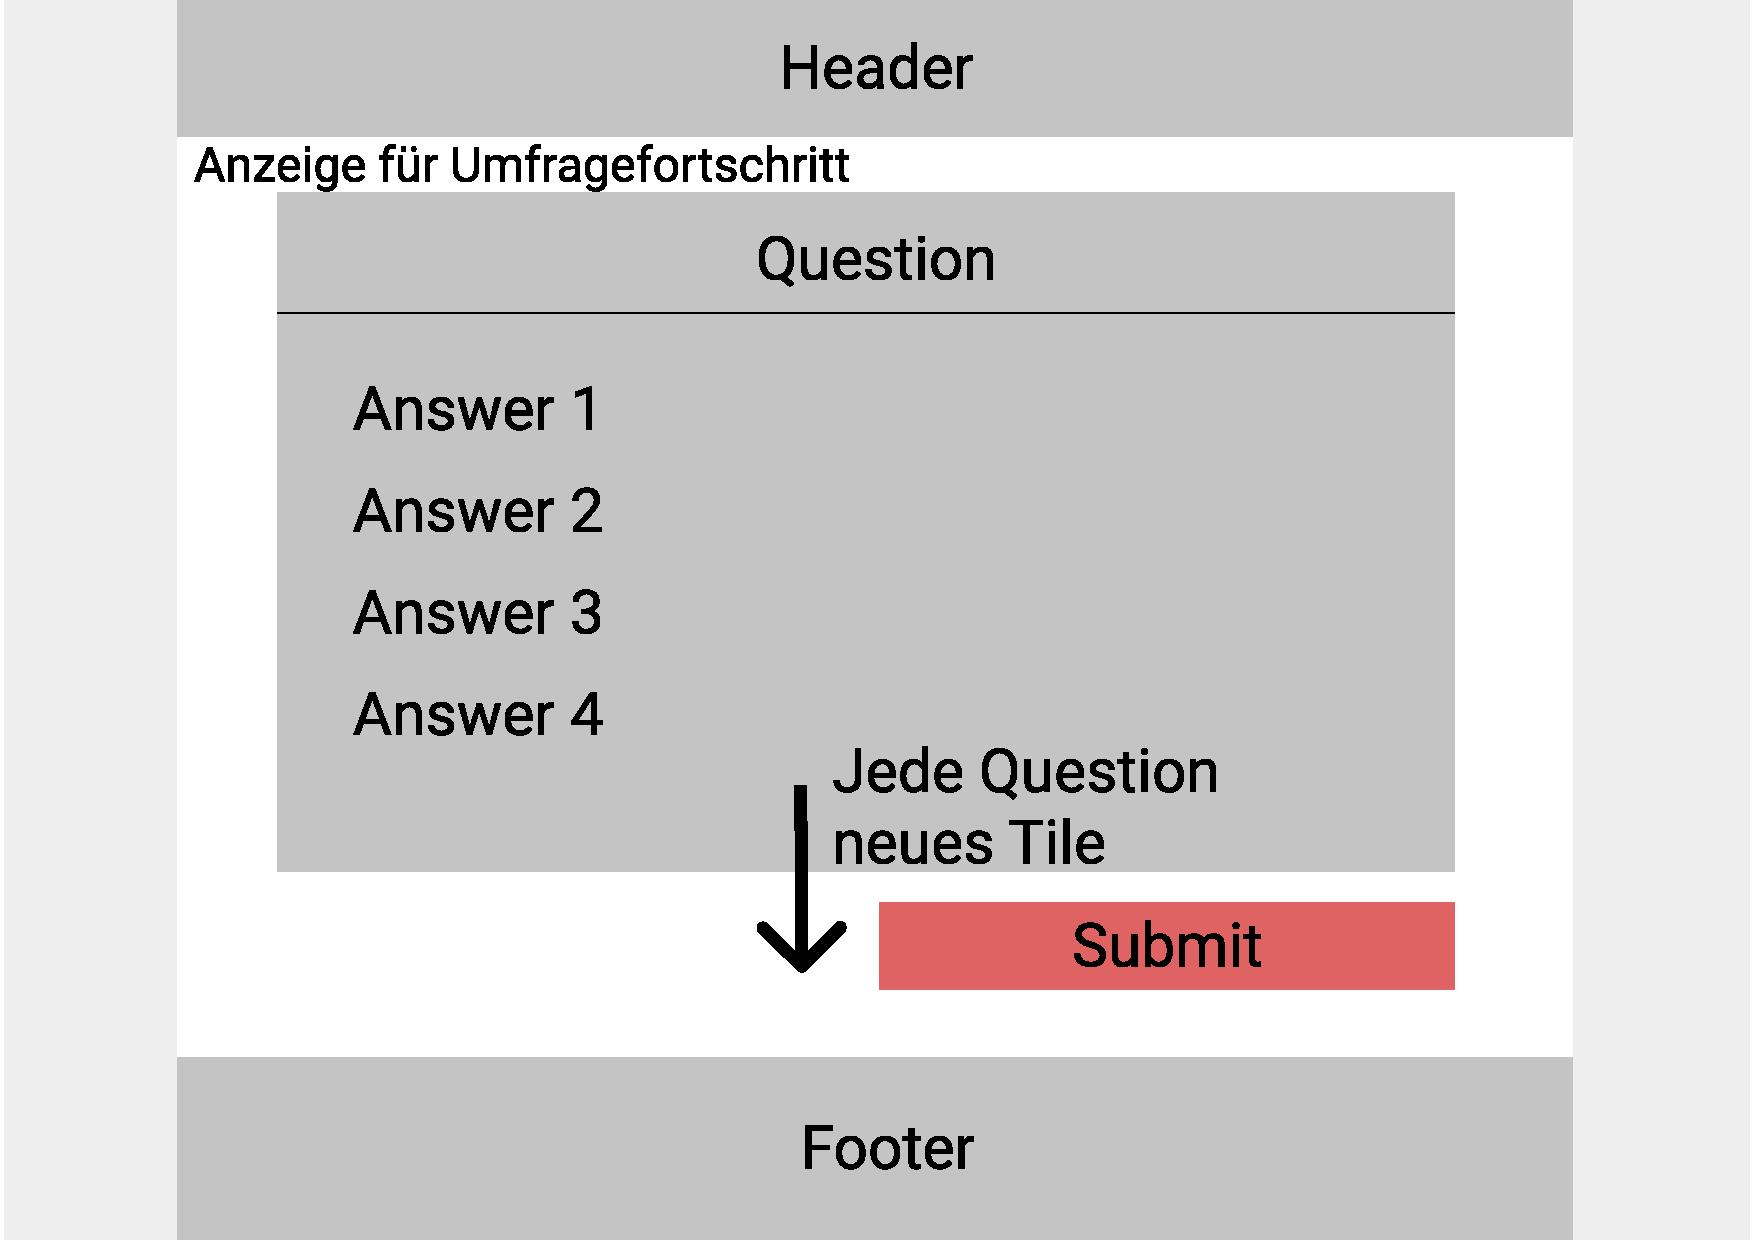
\includegraphics[width=0.7\textwidth]{img/konzeption/client/umfrage_teilnehmer}
	\captionsetup{justification=centering, format=plain}
	\caption[Mock-Up der Teilnahmeseite]{Mock-Up der Teilnahmeseite\\\figma}
	\label{fig:MockUmfrageTeilnehmer}
\end{figure}


\subsection{Result-Dashboard}
\label{ssec:ResultDashboard}





\subsection{Unterteilung der Gliederungsansichten}

\begin{itemize}
	\item Beschreibung der Mockups 
	 \begin{itemize}
		 \item Was haben wir uns bei den einzelnen Seiten gedacht
		 \item Wie sollten die Seiten grundsätzlich aussehen. (Brainstorming)
		 \item evtl. bissel auf Designthinking eingehen
		 \item Welches tool haben wir dazu genutzt
	 \end{itemize}
	 \item Recherche zu vorhandenen Umfragetools --> (https://www.polly.ai/slack-poll, https://strawpoll.de/, https://www.limesurvey.org/de/, https://www.surveymonkey.de/, https://pingo.coactum.de/)
	 --> Ideensammlung und Marktrecherche
	 \item Grundlegende Idee der Einfachheit (evtl Gesamtkonzept)
	 \item Man könnte auf den User Journey eingehen
	 \item Anlehnung an DHBW farben sind vorgesehen
	 \item Orientierung an modernen Websites mit header und footer
	 \item Hinblick auf mobile usage
\end{itemize}
\subsection{Bestimmung von Darstellungsformen}
% !TEX root =  ../../master.tex
\section{Sicherheit}
% !TEX root =  ../../../master.tex
\subsection{Zugriffskontrolle}
Die Zugriffskontrolle erfolgt im Back-End.
Da jegliche Kontrolle, die im Front-End implementiert ist, clientseitig ausgeführt wird, ist sie auch durch einen Angreifer ohne Weiteres aufzuheben und damit als unsicher anzusehen.
Nichtsdestotrotz sind natürlich auch im Front-End entsprechende Maßnahmen implementiert.
Diese dienen allerdings nicht dem Schutz gegen unbefugte Zugriffe, sondern sollen lediglich dafür sorgen, dass Nutzer bereits in der graphischen Darstellung erkennen, wozu sie berechtigt sind und worauf sie Zugriff haben.
Alles andere führt für Benutzer nur zu Verwirrung.

Für die tatsächliche Zugriffskontrolle im Back-End werden, wie bereits in der Konzeption in Abschnitt~\ref{sec:authentifizierung} erläutert, Passwörter beziehungsweise Session-IDs genutzt.
Bei der Registrierung oder einer Anmeldung wird eine solche Session-ID ausgestellt.
Bei jedem Zugriff auf einen der \acs{API}-Endpunkte wird, bevor überhaupt irgendeine Aktion ausgeführt wird, die Korrektheit dieser Session-Id geprüft.
Damit ist sichergestellt, dass eine entsprechende Prüfung nicht versehentlich beim Implementieren eines einzelnen \acs{API}-Endpunkts vergessen werden kann.

Selbstverständlich gibt es auch \acs{API}-Endpunkte, auf die Zugriffe ohne Autorisierung möglich sein müssen.
Dies umfasst einerseits das Beantworten von Umfragen und andererseits das Registrieren und Anmelden, bei dem Nutzer logischerweise noch keine gültige Session-ID besitzen, da sie diese ja dadurch erst erhalten wollen.
Entsprechende Ausnahmen sind über eine Whitelist gelöst, sie werden also explizit aufgelistet.
Auch hierbei steht im Vordergrund, dass \acs{API}-Endpunkte standardmäßig geschützt sind und nicht versehentlich Sicherheitslücken entstehen.

Darüber hinaus wird bei jeder Aktion die Berechtigung geprüft.
Bei der Bearbeitung eines \texttt{SurveyMasters} wird zum Beispiel zuerst einmal validiert, ob dieser auch dem angemeldeten Nutzer zugeordnet ist.

% !TEX root =  ../sicherheit.tex
\subsection{Kommunikation}

\subsubsection{Transferprotokoll}\label{chapter:https}

Um die Sicherheit während der Kommunikation zu erhöhen dürfen Anfragen an den Webserver der Anwendung ausschließlich über \ac{HTTPS} zugelassen werden, sodass  die Kommunikation zwischen Server und Client verschlüsselt wird.
Dies stellt die Integrität der Daten sicher und erhöht damit ebenfalls ihre Vertraulichkeit.
Diese zwei Schutzziele dienen dazu einen potentiellen Angriff, wie etwa einen \ac*{MITM}-Angriff oder einen Lauschangriff, zu verhindern, indem das Ausspähen des Inhalts der Kommunikationspakete durch die vorhandene Verschlüsselung verhindert wird oder etwaige Veränderung der Pakete durch eine fehlerhafte Ent- und erneute Verschlüsselung bemerkt wird.

Zur Verschlüsselung verwendet \ac{HTTPS} die \ac{TLS} und unterscheidet sich grundlegend, neben der \ac{URL}, welche bei der Verwendung von \ac{HTTPS} mit \enquote{https://} beginnt, und der standardmäßigen Nutzung des Port 443, nicht weiter von \ac{HTTP}.

\ac{TLS} setzt dabei auf eine asymmetrische Verschlüsselung, wobei im ersten Schritt ein Schlüsselaustausch zwischen Client und Server vorgesehen ist.
Dies geschieht nach der Version \ac{TLS} 1.3 über drei verschiedene Wege, die aufgrund ihrer Zukunftssicherheit ausgewählt wurden.
Diese Zukunftssicherheit dient dazu, auch langfristige Angriffe zu verhindern, da so nicht alle potentiell von einem Angreifer abgefangenen \ac{TLS}-Sessions entschlüsselt werden können, sobald der private Schlüssel einer Session gefunden wurde.\autocite{rf-RFC8446}

% !TEX root =  ../sicherheit.tex
\subsection{Validierung}

\chapter{Implementierung}
\label{sec:implementierung}
% !TEX root =  ../../master.tex
\section{Server}

\subsection{Grundlegender Aufbau}
Zur Implementierung der Geschäftslogik wird ein Webserver mit Node.js in Verbindung mit dem Framework Express entwickelt.
Bei Node.js handelt es sich um eine JavaScript-Laufzeitumgebung, die die serverseitige Entwicklung mit JavaScript ermöglicht und dabei auf der V8-JavaScript-Implementierung von Google aufsetzt.\autocite[Vgl.][]{nl-openjsfoundation2020nodejs}
Express ist ein Framework für Node.js, um Webanwendungen und \acsp{API} zu entwickeln und wegen der Einfachheit weit verbreitet.\autocite[Vgl.][]{nl-strongloop2017express}

Für die Datenhaltung wird PostgreSQL, ein \ac{RDBMS}, verwendet.
Wie bei allen \acsp{RDBMS} können Daten über die Sprache \acs{SQL} abgefragt und editiert werden.
Mithilfe eines entsprechenden Moduls kann sich innerhalb der Node.js-Anwendung mit der PostgreSQL-Datenbank verbunden werden, sodass \acs{SQL}-Befehle ausgeführt werden können.\autocite[Vgl.][]{nl-carlson2020nodepostgres}

Für jeden \acs{API}-Endpunkt wird jeweils eine Funktion aufgerufen, die die übergebenen Daten entgegennimmt, prüft und daraufhin auf die Datenbank zugreift.

\subsection{Zugriffskontrolle}
Die Zugriffskontrolle erfolgt im Back-End.
Da jegliche Kontrolle, die im Front-End implementiert ist, clientseitig ausgeführt wird, ist sie auch durch einen Angreifer ohne Weiteres aufzuheben und damit als unsicher anzusehen.
Nichtsdestotrotz sind natürlich auch im Front-End entsprechende Maßnahmen implementiert.
Diese dienen allerdings nicht dem Schutz gegen unbefugte Zugriffe, sondern sollen lediglich dafür sorgen, dass Nutzer bereits in der graphischen Darstellung erkennen, wozu sie berechtigt sind und worauf sie Zugriff haben.
Alles andere führt für Benutzer nur zu Verwirrung.

Für die tatsächliche Zugriffskontrolle im Back-End werden, wie bereits in der Konzeption in Abschnitt~\ref{sec:authentifizierung} erläutert, Passwörter beziehungsweise Session-IDs genutzt.
Bei der Registrierung oder einer Anmeldung wird eine solche Session-ID ausgestellt.
Bei jedem Zugriff auf einen der \acs{API}-Endpunkte wird, bevor überhaupt irgendeine Aktion ausgeführt wird, die Korrektheit dieser Session-ID geprüft.
Damit ist sichergestellt, dass eine entsprechende Prüfung nicht versehentlich beim Implementieren eines einzelnen \acs{API}-Endpunkts vergessen werden kann.
Diese entsprechende Funktion ist in Quelltext~\vref{implementation-server-auth-check} abgebildet.

\begin{lstlisting}[language=javascript, caption={Standardmäßige Authentifizierung}, label={lst:implementation-server-auth-check}]
exports.checkUserAuthorization = function (request, callback) {
	const { username, sessionId } = request.body;
	if (username === undefined || sessionId === undefined)
		return callback(false);
	db.query('SELECT * FROM users WHERE lower(username) = lower($1) AND session_id = $2;', [username, sessionId], (err, dbResult) => {
		if (err || dbResult.rows.length !== 1) {
			callback(false);
		} else if (dbResult.rows[0].password_change_required) {
			callback(false, "Error: Password change required");
		} else {
			callback(true);
		}
	});
};
\end{lstlisting}

So wird zunächst der Nutzername und die Session-ID ausgelesen.
Daraufhin kann nach einem entsprechenden Eintrag in der Datenbank gesucht werden.
Wird kein Ergebnis gefunden oder ist ein Passwortwechsel gefordert, so wird der Zugriff verwehrt.

Selbstverständlich gibt es auch \acs{API}-Endpunkte, auf die Zugriffe ohne Autorisierung möglich sein müssen.
Dies umfasst einerseits das Beantworten von Umfragen und andererseits das Registrieren, Passwortwechseln und Anmelden, bei dem Nutzer logischerweise noch keine gültige Session-ID besitzen, da sie diese ja dadurch erst erhalten wollen.
Entsprechende Ausnahmen sind über eine Whitelist gelöst, sie werden also explizit aufgelistet.
Auch hierbei steht im Vordergrund, dass \acs{API}-Endpunkte standardmäßig geschützt sind und nicht versehentlich Sicherheitslücken entstehen.

Darüber hinaus wird bei jeder Aktion die Berechtigung geprüft.
Bei der Bearbeitung eines \texttt{SurveyMasters} wird zum Beispiel zuerst einmal validiert, ob dieser auch dem angemeldeten Nutzer zugeordnet ist.

% !TEX root =  ../../master.tex
\section{Client}
\authorsection{\authorSG}

Wie bereits in Kap. \vref{ssec:React} beschrieben, wird in diesem Projekt React verwendet. 
Für die Unterteilung der verschiedenen Komponenten soll auf eine spezielle \acfp{UX} und \acfp{UI} gelegt werden. 
Im folgenden soll auf den Aufbau der Benutzeroberfläche eingegangen werden. 

\subsection{Participate}
Im Bezug auf Verwendbarkeit wie in Kap. \vref{sec:UserJourney} beschrieben ist die Startseite die \emph{Participate}-Seite. 
In dieser soll der Benutzer bzw. Student der an einer Umfrage teilnimmt, einen \emph{Surveycode} wie z.B. \emph{\texttt{OYZQGGXOF9}} eingeben, um an der Umfrage zu partizipieren. 

Anschließend wird der Benutzer auf die Umfrageseite weitergeleitet, auf der er die benötigten Felder ausfüllt (siehe \vref{ssec:Umfrage}).

\subsection{Umfrage}
\label{ssec:konzept:client:umfrage}
Wie in Abbildung~\vref{fig:MockUmfrageTeilnehmer} dargestellt, wird der Teilnehmer auf die zuvor angegebene Umfrage geleitet.
Die Fragen werden dabei jeweils in einer eigenen Karte dargestellt.
Durch Drücken eines Knopfes soll der Teilnehmer zur nächsten Frage gelangen.
Gleichzeitig soll dem Benutzer sein Fortschritt verdeutlicht werden, um die Dauer der Umfrage abschätzen zu können.
Die Abgabe der Umfrage erfolgt identisch zum Fragenwechsel.
Der Teilnehmer soll dabei Feedback erhalten, ob seine Teilnahme erfolgreich war.

Durch diesen Vorgang sollen die Anforderungen~\hyperref[Anf:A14]{A14}, die anonyme Teilnahme, sowie \hyperref[Anf:15]{A15}, die einfache Teilnahme an einer Umfrage, erfüllt werden.

\begin{figure}[H]
	\centering
	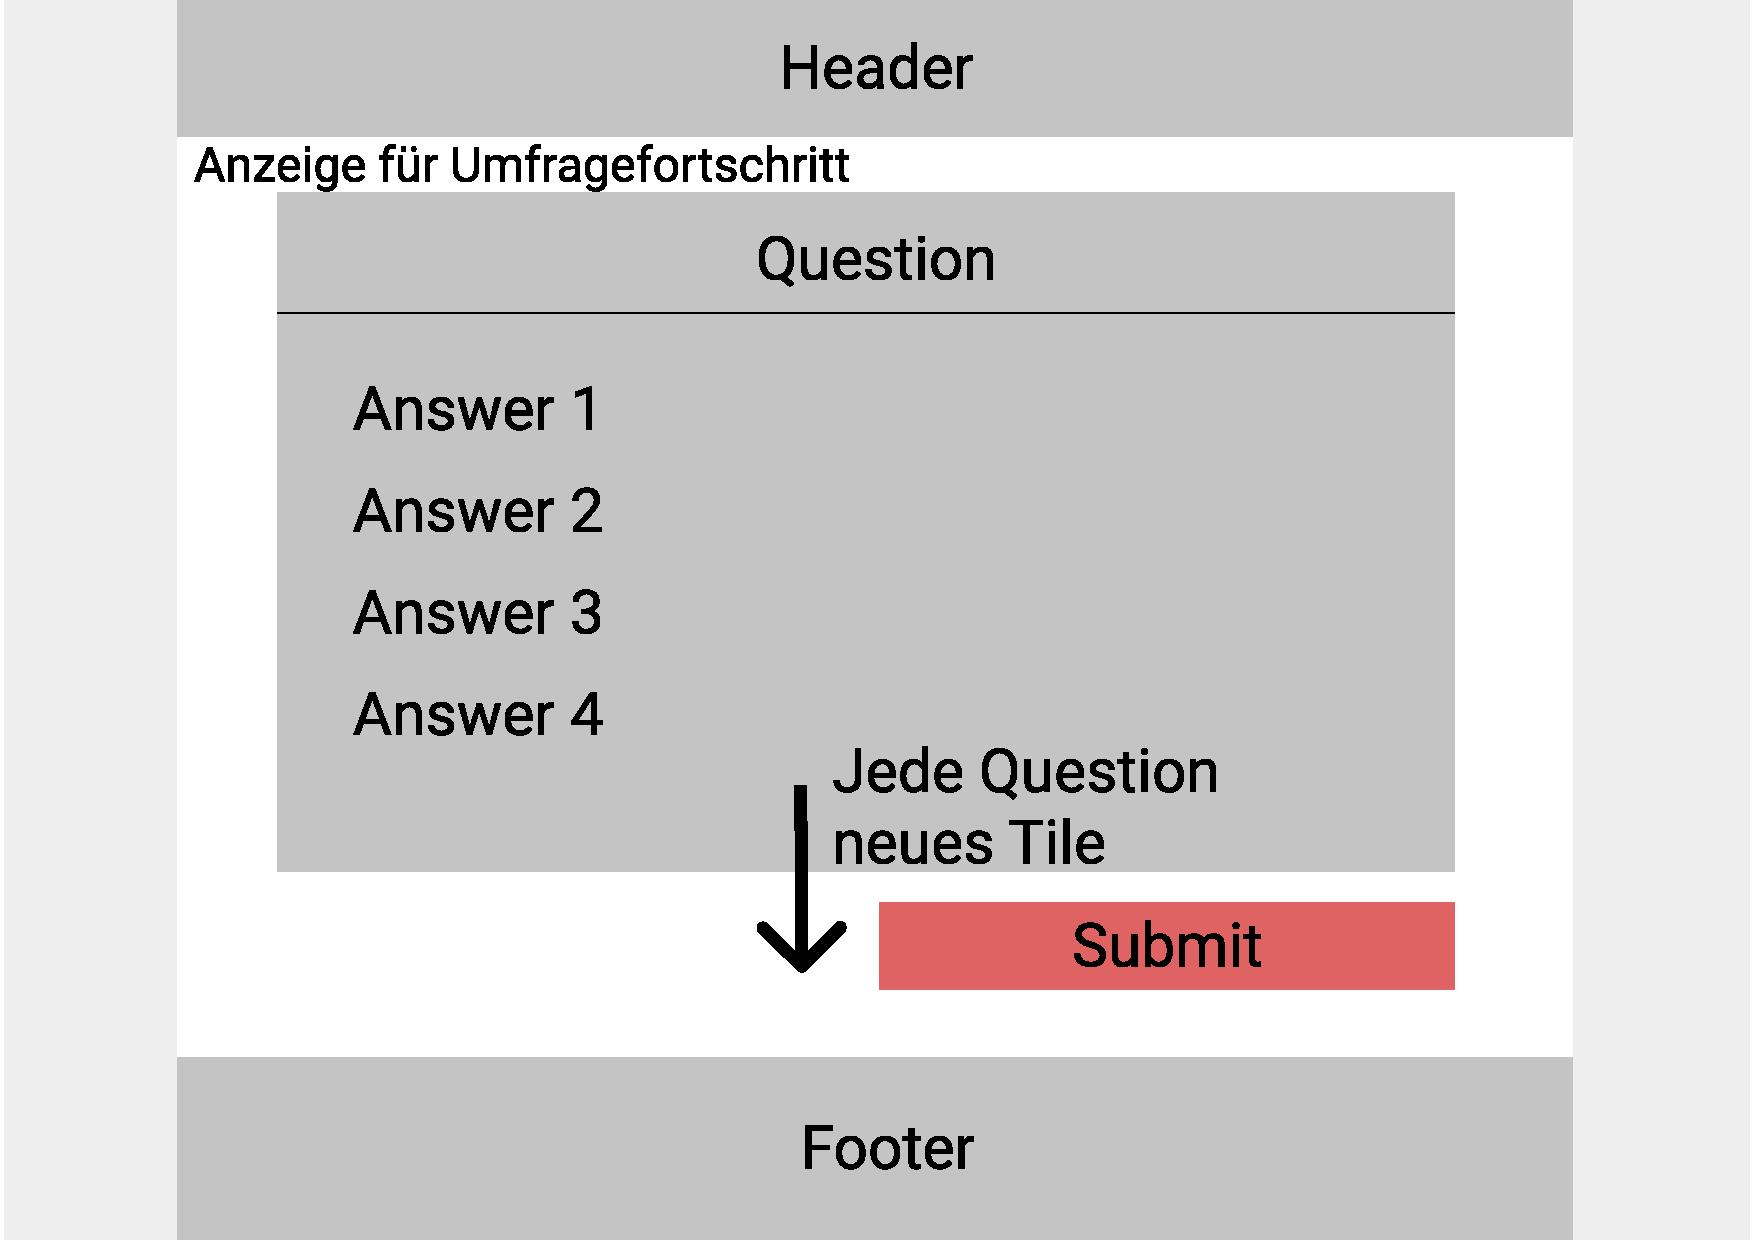
\includegraphics[width=0.7\textwidth]{img/konzeption/client/umfrage_teilnehmer}
	\captionsetup{justification=centering, format=plain}
	\caption[Mock-Up der Teilnahmeseite]{Mock-Up der Teilnahmeseite\\\figma}
	\label{fig:MockUmfrageTeilnehmer}
\end{figure}


\subsection{Result-Dashboard}
\label{ssec:ResultDashboard}





\subsection{Unterteilung der Gliederungsansichten}

\begin{itemize}
	\item Beschreibung der Mockups 
	 \begin{itemize}
		 \item Was haben wir uns bei den einzelnen Seiten gedacht
		 \item Wie sollten die Seiten grundsätzlich aussehen. (Brainstorming)
		 \item evtl. bissel auf Designthinking eingehen
		 \item Welches tool haben wir dazu genutzt
	 \end{itemize}
	 \item Recherche zu vorhandenen Umfragetools --> (https://www.polly.ai/slack-poll, https://strawpoll.de/, https://www.limesurvey.org/de/, https://www.surveymonkey.de/, https://pingo.coactum.de/)
	 --> Ideensammlung und Marktrecherche
	 \item Grundlegende Idee der Einfachheit (evtl Gesamtkonzept)
	 \item Man könnte auf den User Journey eingehen
	 \item Anlehnung an DHBW farben sind vorgesehen
	 \item Orientierung an modernen Websites mit header und footer
	 \item Hinblick auf mobile usage
\end{itemize}
\subsection{Bestimmung von Darstellungsformen}
% !TEX root =  ../../master.tex
\section{Sicherheit}
% !TEX root =  ../../../master.tex
\subsection{Zugriffskontrolle}
Die Zugriffskontrolle erfolgt im Back-End.
Da jegliche Kontrolle, die im Front-End implementiert ist, clientseitig ausgeführt wird, ist sie auch durch einen Angreifer ohne Weiteres aufzuheben und damit als unsicher anzusehen.
Nichtsdestotrotz sind natürlich auch im Front-End entsprechende Maßnahmen implementiert.
Diese dienen allerdings nicht dem Schutz gegen unbefugte Zugriffe, sondern sollen lediglich dafür sorgen, dass Nutzer bereits in der graphischen Darstellung erkennen, wozu sie berechtigt sind und worauf sie Zugriff haben.
Alles andere führt für Benutzer nur zu Verwirrung.

Für die tatsächliche Zugriffskontrolle im Back-End werden, wie bereits in der Konzeption in Abschnitt~\ref{sec:authentifizierung} erläutert, Passwörter beziehungsweise Session-IDs genutzt.
Bei der Registrierung oder einer Anmeldung wird eine solche Session-ID ausgestellt.
Bei jedem Zugriff auf einen der \acs{API}-Endpunkte wird, bevor überhaupt irgendeine Aktion ausgeführt wird, die Korrektheit dieser Session-Id geprüft.
Damit ist sichergestellt, dass eine entsprechende Prüfung nicht versehentlich beim Implementieren eines einzelnen \acs{API}-Endpunkts vergessen werden kann.

Selbstverständlich gibt es auch \acs{API}-Endpunkte, auf die Zugriffe ohne Autorisierung möglich sein müssen.
Dies umfasst einerseits das Beantworten von Umfragen und andererseits das Registrieren und Anmelden, bei dem Nutzer logischerweise noch keine gültige Session-ID besitzen, da sie diese ja dadurch erst erhalten wollen.
Entsprechende Ausnahmen sind über eine Whitelist gelöst, sie werden also explizit aufgelistet.
Auch hierbei steht im Vordergrund, dass \acs{API}-Endpunkte standardmäßig geschützt sind und nicht versehentlich Sicherheitslücken entstehen.

Darüber hinaus wird bei jeder Aktion die Berechtigung geprüft.
Bei der Bearbeitung eines \texttt{SurveyMasters} wird zum Beispiel zuerst einmal validiert, ob dieser auch dem angemeldeten Nutzer zugeordnet ist.

% !TEX root =  ../sicherheit.tex
\subsection{Kommunikation}

\subsubsection{Transferprotokoll}\label{chapter:https}

Um die Sicherheit während der Kommunikation zu erhöhen dürfen Anfragen an den Webserver der Anwendung ausschließlich über \ac{HTTPS} zugelassen werden, sodass  die Kommunikation zwischen Server und Client verschlüsselt wird.
Dies stellt die Integrität der Daten sicher und erhöht damit ebenfalls ihre Vertraulichkeit.
Diese zwei Schutzziele dienen dazu einen potentiellen Angriff, wie etwa einen \ac*{MITM}-Angriff oder einen Lauschangriff, zu verhindern, indem das Ausspähen des Inhalts der Kommunikationspakete durch die vorhandene Verschlüsselung verhindert wird oder etwaige Veränderung der Pakete durch eine fehlerhafte Ent- und erneute Verschlüsselung bemerkt wird.

Zur Verschlüsselung verwendet \ac{HTTPS} die \ac{TLS} und unterscheidet sich grundlegend, neben der \ac{URL}, welche bei der Verwendung von \ac{HTTPS} mit \enquote{https://} beginnt, und der standardmäßigen Nutzung des Port 443, nicht weiter von \ac{HTTP}.

\ac{TLS} setzt dabei auf eine asymmetrische Verschlüsselung, wobei im ersten Schritt ein Schlüsselaustausch zwischen Client und Server vorgesehen ist.
Dies geschieht nach der Version \ac{TLS} 1.3 über drei verschiedene Wege, die aufgrund ihrer Zukunftssicherheit ausgewählt wurden.
Diese Zukunftssicherheit dient dazu, auch langfristige Angriffe zu verhindern, da so nicht alle potentiell von einem Angreifer abgefangenen \ac{TLS}-Sessions entschlüsselt werden können, sobald der private Schlüssel einer Session gefunden wurde.\autocite{rf-RFC8446}

% !TEX root =  ../sicherheit.tex
\subsection{Validierung}

\chapter{Ausblick}
% !TEX root =  ../../master.tex
\section{Fazit zur Gruppen- und Seminararbeit}
\label{sec:Fazit}

Bei der Arbeit handelt es sich um die Dokumentation der Verwendung und Neuentwicklung einer Webapplikation. 
Von den verwendten Grundlagen, sowohl aus technischer und theoretischer Sicht, bis hin zu einem Nutzerhandbuch, wurden alle Schritte zur Erstellung der Anwendung beschrieben. 
Die einzelnen Schritte der Konzeption und Implementierung sind ausführlich erläutert, um die Überlegungen hinter den einzelnen Entscheidungen zu begründen. 


Im Rahmen der Seminararbeit wurde eine Webanwendung zur Umfrageerstellung, -verwaltung und -ausführung erstellt.
Weiterhin wurde ein Benutzerverwaltungskonzept in die Anwendung integriert, um geforderte Anforderungen zu erfüllen.

- Kurze Zusammenfassung
    - Grundlagen - Konzeption - Implementierung - Nutzerhandbuch - Fazit
    - Umfragetool nach den Anforderungen gebaut
    - Verbesserungen eingebaut
    - Dokumentation für die Verwendung und Weiterentwicklung von der Webapplikation

- Warum und wie das Ziel erreicht wurde
    - Anforderungen ALLE erfüllt und mehr als nur zur vollstädnigkeit erreicht
    - 
% !TEX root =  ../../master.tex
\section{Ausblick}
\label{sec:Ausblick}

Die Applikation hat noch nicht ihren vollen Umfang erreicht.
Sie zeigt derzeit einen soliden Stand mit dem Hauptaugenmerk des Erstellen von Umfragen von verschiedenen Benutzern.

\subsubsection*{Forum}
Sinnvoll wäre es, eine Art Forum, ähnlich einem Diskussionsforum der Applikation, anzufügen.
Hintergrund ist, dass \zb Dozenzen wie \dutzi ein Forumseintrag machen können, um hier Diskussionen zu führen.
So könnten die Teilnehmer aus dem Kurs wie \weigert über die Fragestellung diskutieren.
Andererseits könnten sich Studierende dort auch über verschiedene Themenbereich zur Prüfungsvorbereitung austauschen und hier Dokumente teilen. \newline
Um dies zu realisieren, müssten Datenbankanpassungen vorgenommen werden, um das Forum darzustellen und auch weitere Benutzer als Student dem System hinzufügen.
Wichtig hierbei ist, dass es zu jedem Forum mehrere Forumseinträge geben kann.
Jeder Forumseintrag wird von einem Benutzer verfasst. \newline
So kann \dutzi sehen ob \weigert einen Eintrag gestellt hat.
Gegebenenfalls könnten \dutzi und \weigert auch direkt miteinander schreiben.

\subsubsection*{Individual-Chat \& Gruppenchat}
Ein interessantes Themenfeld ist das Thema Chat in einer Anwendung.
So ist vorstellbar, dass die Anwendung über eine Chatfunktion verfügt.
Studierende könnten sich hier in Gruppenchats oder per Direktchat austauschen.
Ein weiteres denkbares Feature ist der 1:1-Chat von Dozierenden und Studierenden.
So könnte sich \weigert mit seinen Fragen an \dutzi wenden, um kleinere Fragen zu stellen. \newline
Hierfür sollten die Benutzer über einen geeigneten Benutzernamen verfügen, um auch bei einer Abwesenheit auf seine Chatnachrichten zuzugreifen.


% bibliography
\setcounter{biburllcpenalty}{7000}
\setcounter{biburlucpenalty}{8000}
\clearpage
\ihead{}
\printbibliography[title=Literaturverzeichnis]
\cleardoublepage

% appendix
\appendix
\ihead{\appendixname~\thechapter}

\chapter{Abbildungen}
\begin{sidewaysfigure}[ht]
	\centering
	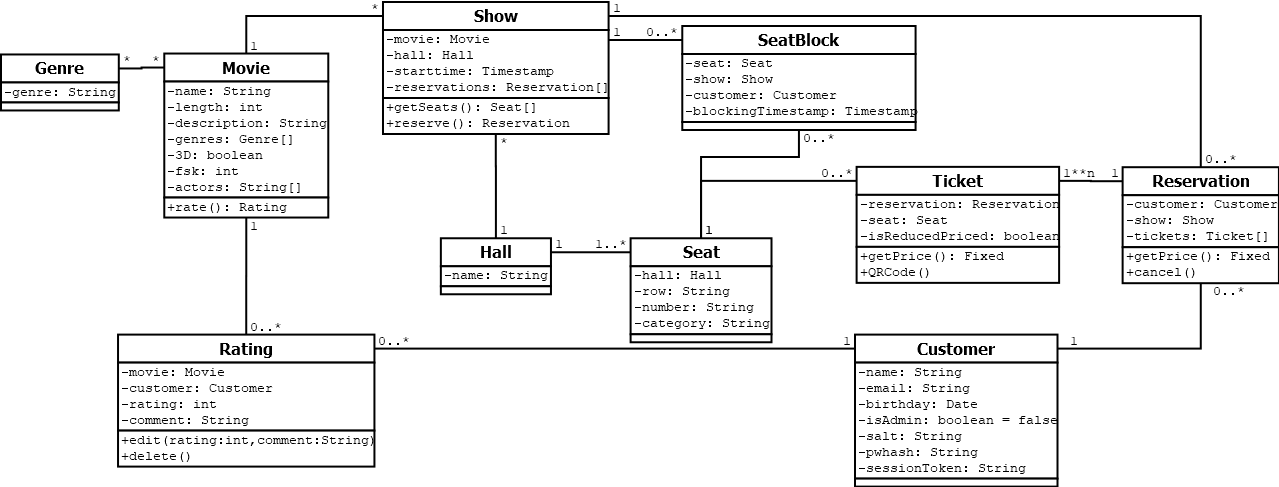
\includegraphics[keepaspectratio, width=\textwidth, height=\textheight]{img/klassendiagramm_v01}
	\captionsetup{format=hang}
	\caption{Erster Entwurf des Klassendiagramms}
	\small Quelle: eigene Darstellung mittels \url{http://dia-installer.de/index.html.de}
	\label{fig:anhang_klassendiagramm01}
\end{sidewaysfigure}

\begin{sidewaysfigure}[ht]
	\centering
	
\includegraphics[keepaspectratio, width=\textwidth, height=\textheight]{img/klassendiagramm_v02}
	\captionsetup{format=hang}
	\caption{Zweiter Entwurf des Klassendiagramms}
	\small Quelle: eigene Darstellung mittels \url{https://draw.io/} 
	\label{fig:anhang_klassendiagramm02}
\end{sidewaysfigure}

\begin{sidewaysfigure}[ht]
	\centering
	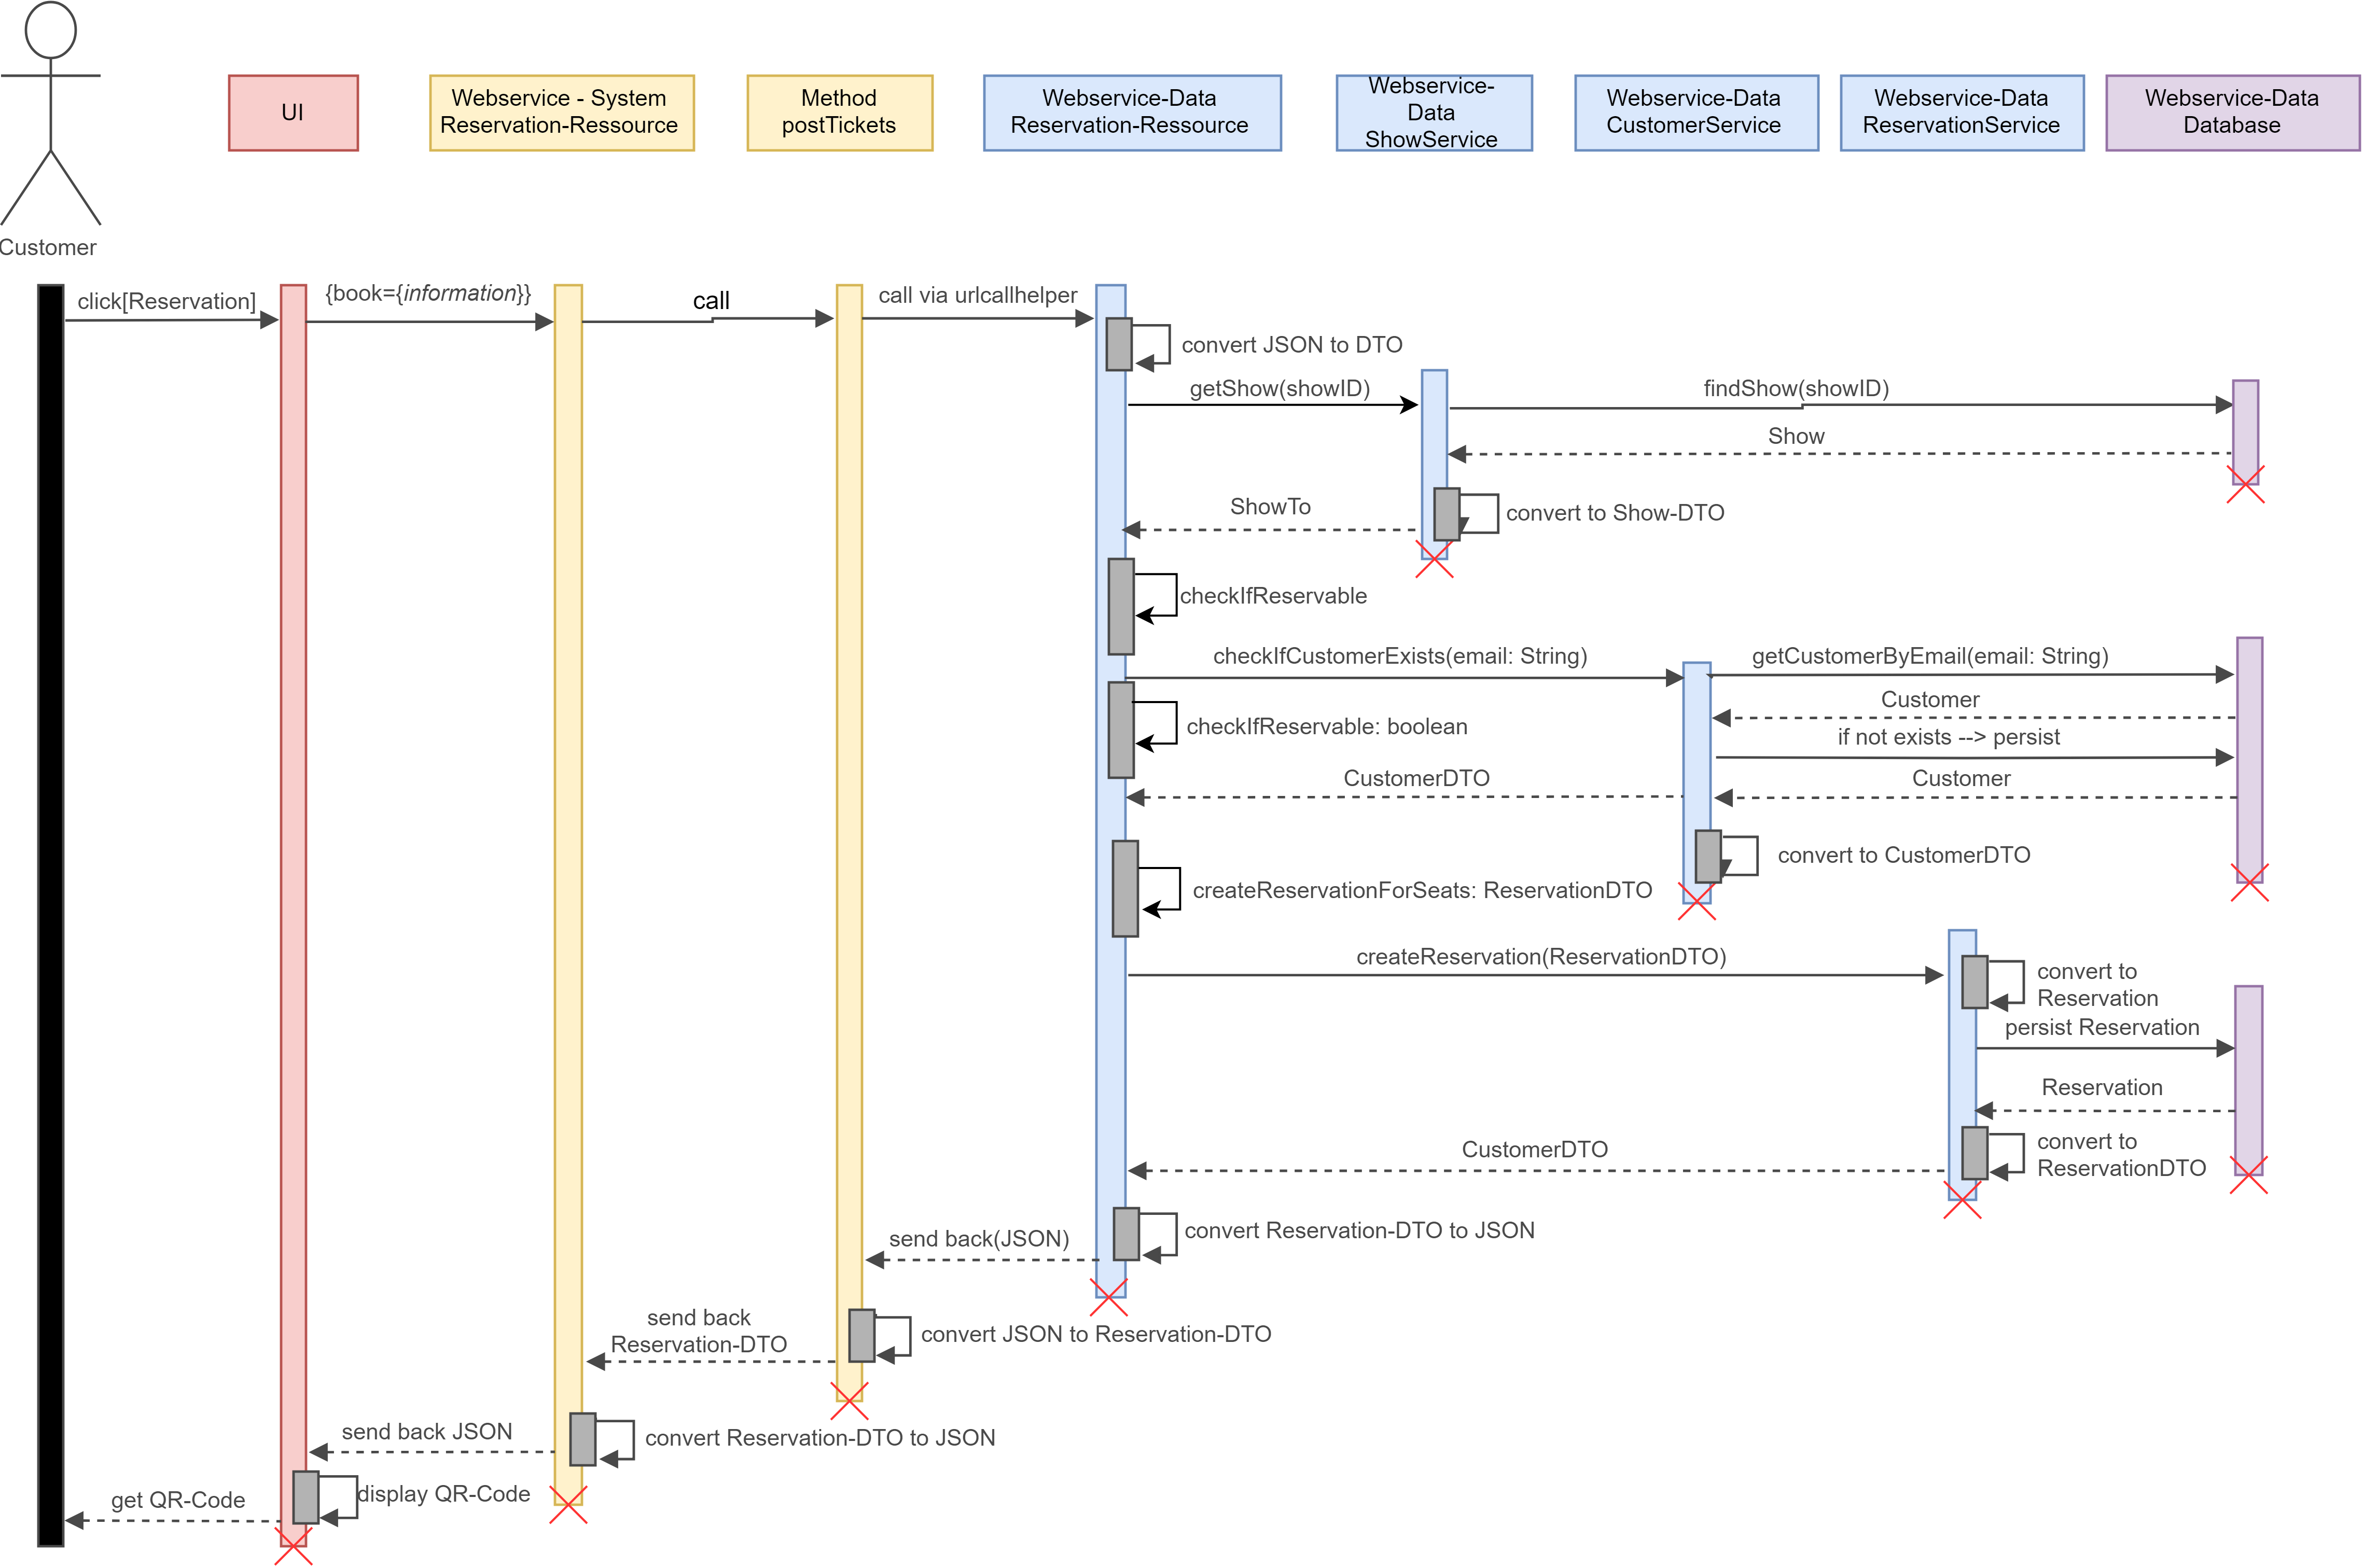
\includegraphics[keepaspectratio, width=\textwidth, height=\textheight]{img/sequenzdiagramm_reservation}
	\captionsetup{format=hang}
	\caption{Sequenzdiagramm eines Reservierungsvorganges}
	\small Quelle: eigene Darstellung mittels \url{https://draw.io/} 
	\label{fig:Anhang_seq_reservieren}
\end{sidewaysfigure}

\begin{sidewaysfigure}[ht]
	\centering
	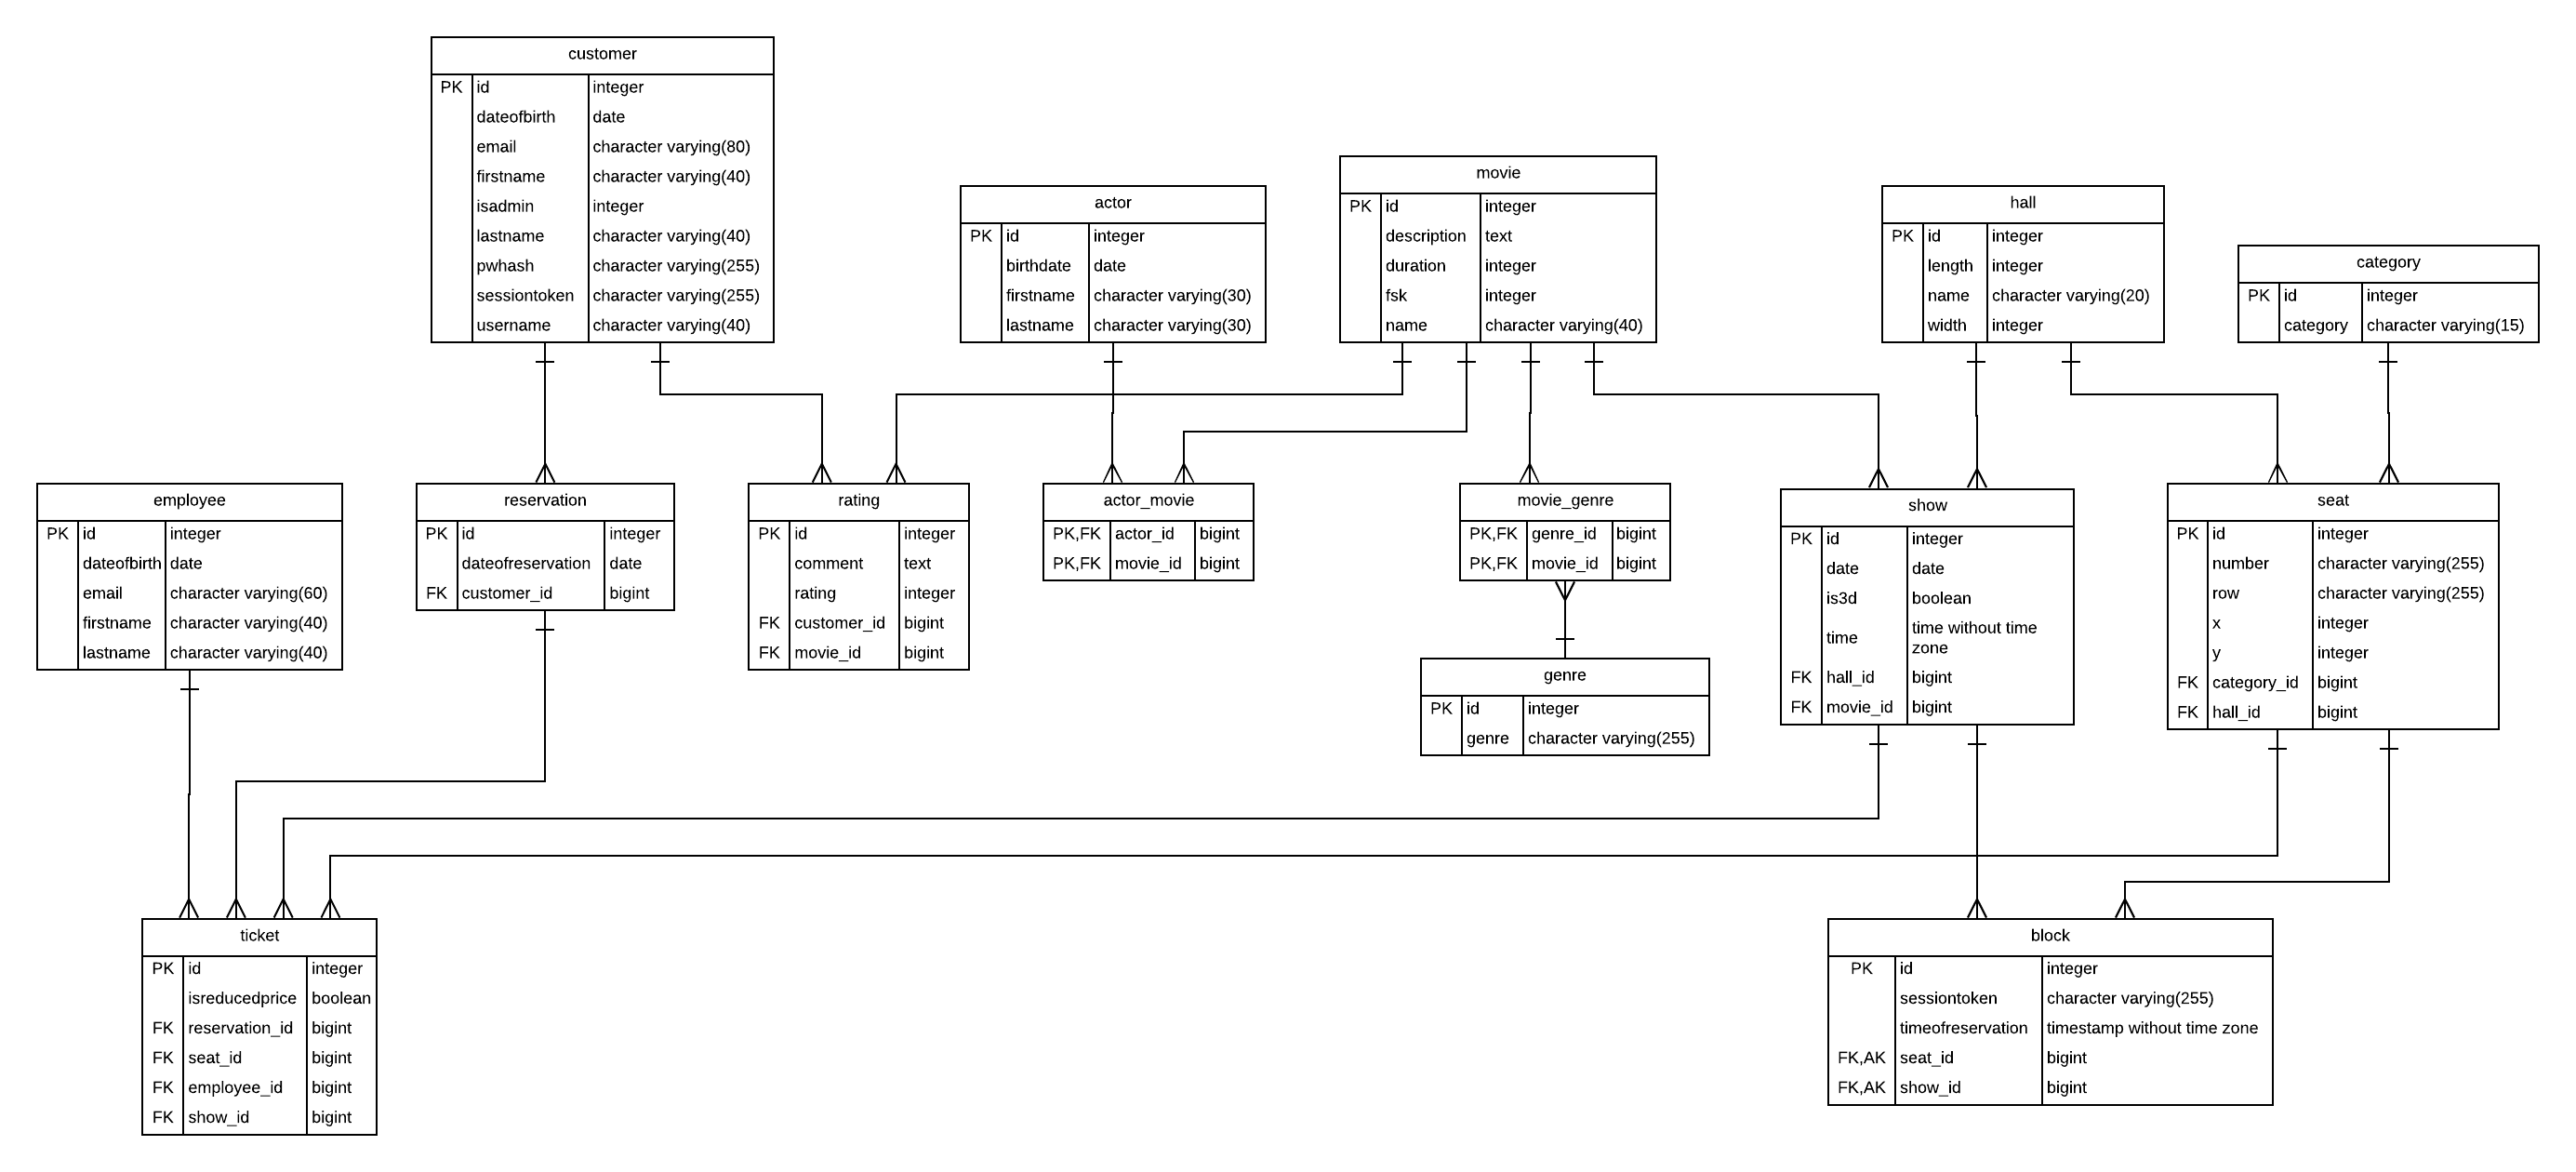
\includegraphics[keepaspectratio, width=\textwidth, height=\textheight]{img/ER-Modell}
	\captionsetup{format=hang}
	\caption{\acs{ER-Modell} der Datenbank}
	\small Quelle: eigene Darstellung mittels \url{https://www.lucidchart.com/}
	\label{fig:Anhang_ER-Modell}
\end{sidewaysfigure}

\chapter{Screenshots aus dem Front-End}
\label{sec:screenshots_frontend}
Die folgenden Screenshots sind alle von der Seite eines Filmes, auf der sich weitere Details zu diesem finden.

\begin{figure}[ht]
	\centering
	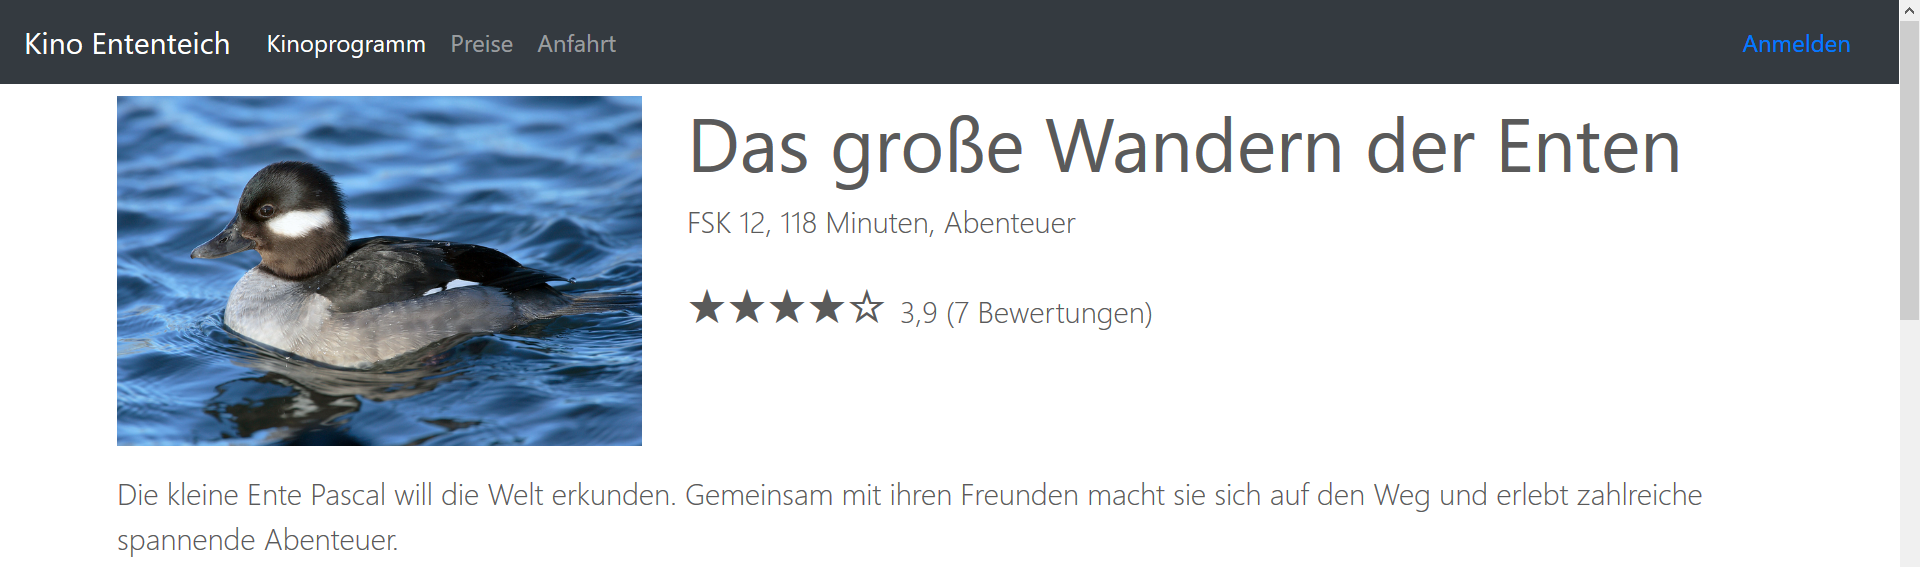
\includegraphics[width=\textwidth]{img/screenshots/film02a}
	\captionsetup{format=hang}
	\caption{Filmdetails}
	\label{fig:film02a}
\end{figure}

\begin{figure}[ht]
	\centering
	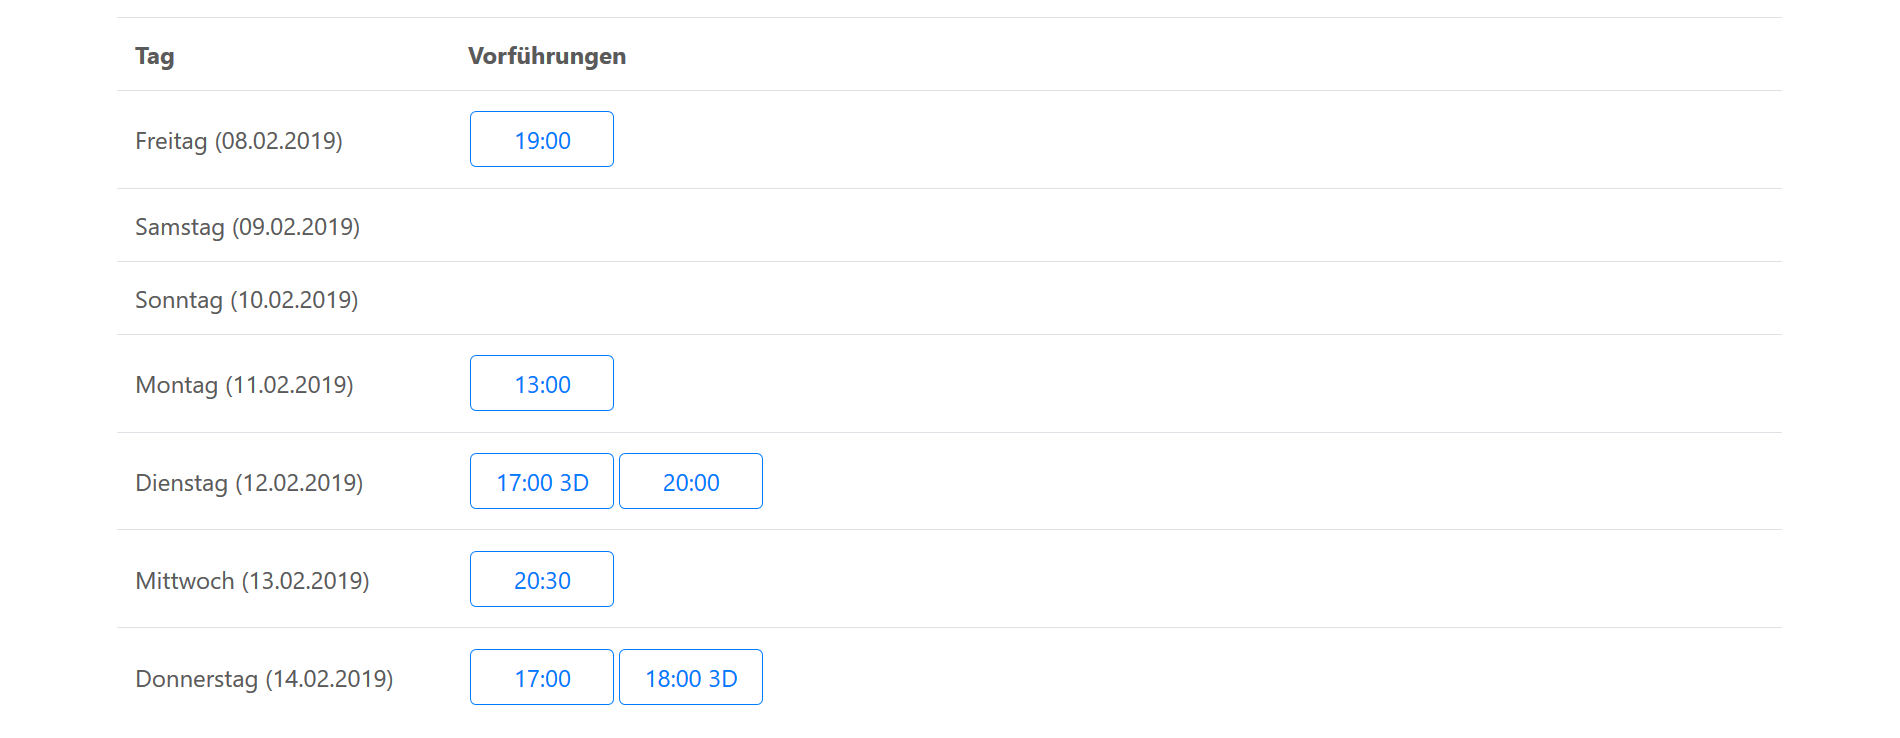
\includegraphics[width=\textwidth]{img/screenshots/film03}
	\captionsetup{format=hang}
	\caption{Liste der Vorstellungen der nächsten 7 Tage}
	\label{fig:film03}
\end{figure}

\begin{figure}[!t]
	\centering
	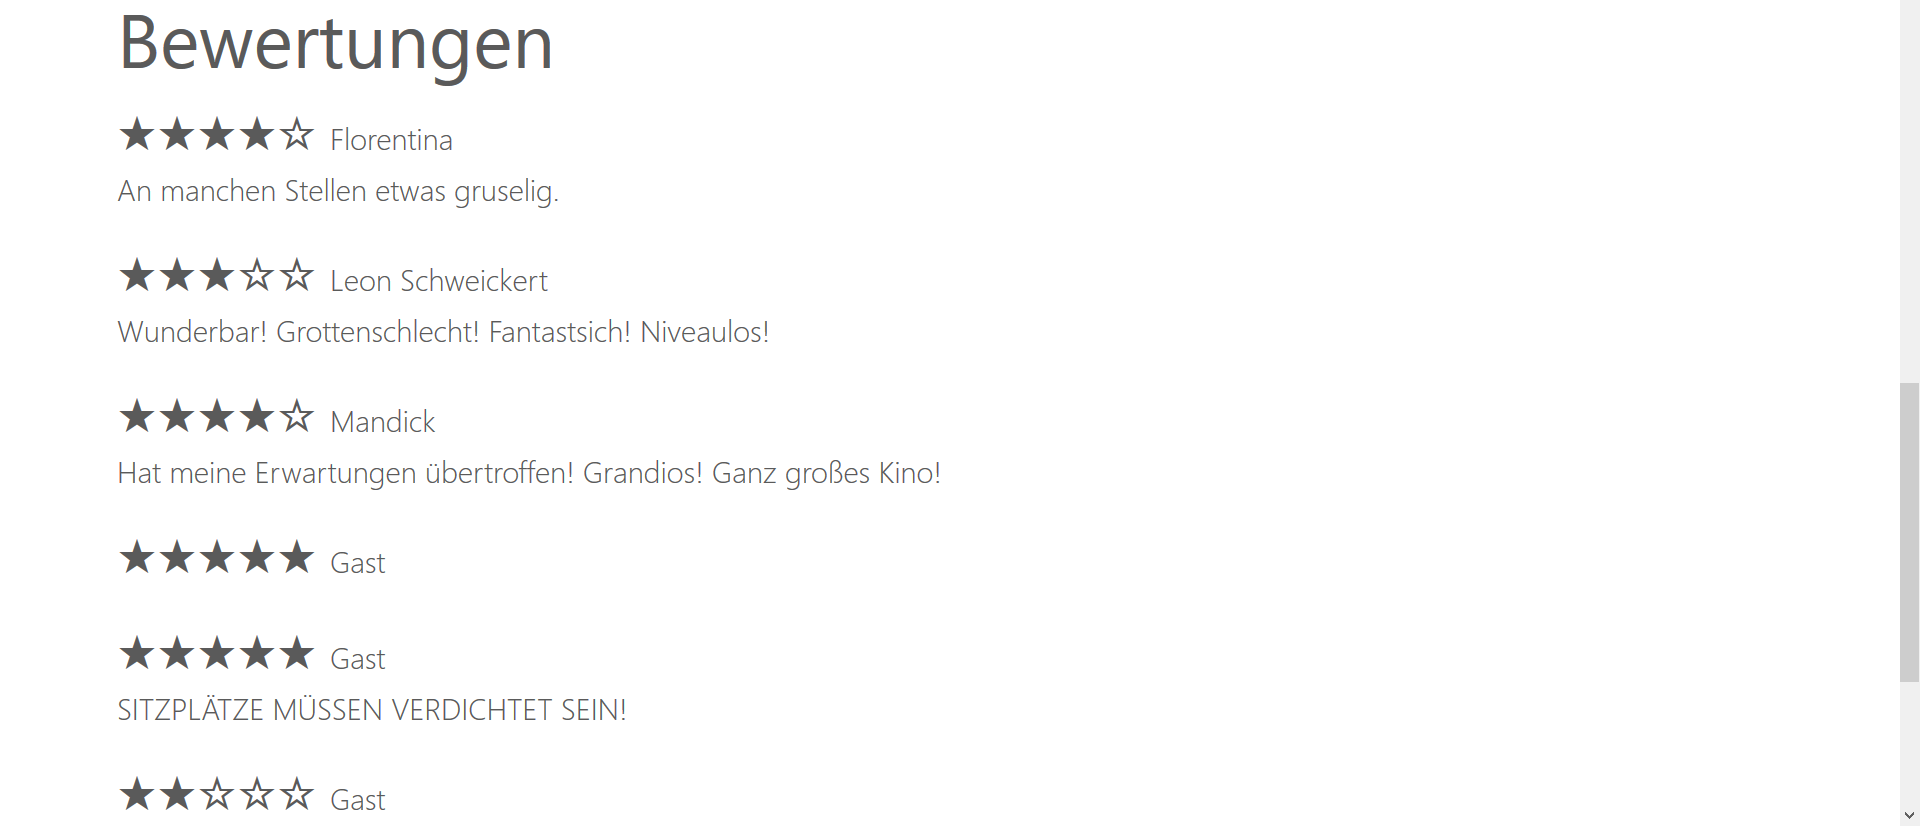
\includegraphics[width=\textwidth]{img/screenshots/film04}
	\captionsetup{format=hang}
	\caption{Bewertungen zu einem Film}
	\label{fig:film04}
\end{figure}

\chapter{Quellcode}

\begin{lstlisting}[style=lstJava, caption={Erstellen eines Movie-\acs{DTO}s aus einer Movie-Entität mit Hilfe des eigen erstellten EntityToToHelper}, label={lst:EntityToToHelper_movie}]
public static MovieTo createMovieTo ( Movie entity, boolean withShow )
{
	if ( null != entity )
	{
		MovieTo movieTo = new MovieTo();
		movieTo.setId(entity.getId());
		movieTo.setDescription(entity.getDescription());
		movieTo.setFsk(entity.getFsk());
		movieTo.setDuration(entity.getDuration());
		movieTo.setName(entity.getName());
		movieTo.setGenres(createGenreTos(entity.getGenres()));
		movieTo.setRatings(createRatingTos(entity.getRatings()));
		if ( withShow )
		{
			movieTo.setShows(createShowTos(entity.getShows(), false));
		} // end withSow
		movieTo.setActors(createActorTos(entity.getActors()));
		return movieTo;
	}  // end if null
	return null;
}
\end{lstlisting}

\newpage

\begin{lstlisting}[style=lstJava, caption={Erstellen einer Movie-Entität aus einem Movie-\acs{DTO} mit Hilfe des eigen erstellten ToToEntityHelper}, label={lst:ToToEntityHelper_movie}]
public static Movie createMovieEntity ( MovieTo transferObject, boolean withShow )
{
	if ( null != transferObject )
	{
		Movie movie = new Movie();
		movie.setId(transferObject.getId());
		movie.setActors(createActorEntities(transferObject.getActors()));
		movie.setDescription(transferObject.getDescription());
		movie.setFsk(transferObject.getFsk());
		movie.setDuration(transferObject.getDuration());
		movie.setName(transferObject.getName());
		movie.setRatings(createRatingEntities(transferObject.getRatings()));
		if ( withShow )
		{
			movie.setShows(createShowEntities(transferObject.getShows(), false));
		}
		movie.setGenres(createGenreEntities(transferObject.getGenres()));
		return movie;
	}
	return null;
}
\end{lstlisting}

\newpage

\begin{lstlisting}[style=lstJava, caption={Überprüfung, ob eine Reservierung möglich ist}, label={lst:Angang_Prüfung_ob_Reservierung_möglich}, tabsize=2]
private boolean checkIfSeatsAreBookable ( List<SeatTo> seatsToProof, List<TicketTo> bookedTicketTos, List<BlockTo> blockTos, String sessiontoken ) {
	boolean bookable = true;
	
	for ( SeatTo s : seatsToProof ) {
		if ( bookable ) {
			for ( TicketTo t : bookedTicketTos ) {
				if ( s.getId() == t.getSeat().getId() ) {
					bookable = false;
					s.setOccupied(true);
					break;
				}
				else {
					s.setOccupied(false);
				}
			} // end for ticket

			// verification for blocked elements
			for ( BlockTo b : blockTos ) {
				if ( s.getId() == b.getSeat().getId() &&
				     !(b.getSessiontoken().equals(sessiontoken)) ) {
					bookable = false;
					s.setBlocked(true);
					break;
				}
				else {
					s.setBlocked(false);
				}
			} // end for block
		}	// end if bookable
	}	// end for seatTo

	return bookable;
}
\end{lstlisting}

\newpage

\begin{lstlisting}[style=lstJava, caption={Erstellen eines Reservierungs-\acs{DTO}s}, label={lst:Anhang_Erstellen_Reservierung}]
private ReservationTo createReservationForSeats ( List<SeatTo> seatTos, ShowTo showTo )
{
	List<TicketTo> toBook = new ArrayList<>();
	ReservationTo createdReservationTo = new ReservationTo();
		
	for ( SeatTo seatTo : seatTos )
	{
		seatTo.setOccupied(true);
	
		TicketTo ticketTo = new TicketTo();
		ticketTo.setSeat(seatTo);
		ticketTo.setShow(showTo);
		ticketTo.setReservation(createdReservationTo);
		if ( seatTo.isReducedPrice() )
		{
			ticketTo.setReducedPrice(true);
		}
		toBook.add(ticketTo);
	}
	createdReservationTo.setDateOfReservation(Utils.convertDateToString(new Date()));
	createdReservationTo.setTickets(toBook);
	return createdReservationTo;
}
\end{lstlisting}

\newpage

\begin{lstlisting}[style=lstJava, caption={Ausschnitt der Test-Klasse der EntityToToHelper-Klasse}, label={src:entitytotohelpertest}, tabsize=2]
public class EntityToToHelper_Test {
	EntityToToHelper EtoToHelper = new EntityToToHelper();

	@Before
	public void initialize ( ) {
		EmployeeTo testEmployeeTo = new EmployeeTo();
		testEmployeeTo.setId(1);
		testEmployeeTo.setDateofbirth(testDateString);
		testEmployeeTo.setEmail("mail");
		testEmployeeTo.setFirstname("firstname");
		testEmployeeTo.setLastname("lastname");

		Employee testEmployeeEntity = new Employee();
		testEmployeeEntity.setId(1);
		testEmployeeEntity.setDateofbirth(testDateDate);
		testEmployeeEntity.setEmail("mail");
		testEmployeeEntity.setFirstname("firstname");
		testEmployeeEntity.setLastname("lastname");
	}

	@Test
	public void testCreateEmployeeTo ( ) {
		assertEquals(null, EtoToHelper.createEmployeeTo(null));

		EmployeeTo compareEmployeeTo = EtoToHelper.createEmployeeTo(testEmployeeEntity);

		assertThat(testEmployeeTo.getId(), equalTo(compareEmployeeTo.getId()));
		assertThat(testEmployeeTo.getDateofbirth(), equalTo(compareEmployeeTo.getDateofbirth()));
		assertThat(testEmployeeTo.getEmail(), equalTo(compareEmployeeTo.getEmail()));
		assertThat(testEmployeeTo.getFirstname(), equalTo(compareEmployeeTo.getFirstname()));
		assertThat(testEmployeeTo.getLastname(), equalTo(compareEmployeeTo.getLastname()));
	}
}
\end{lstlisting}


% ewerkl.tex
% !TEX root =  master.tex

\clearpage
\chapter*{Ehrenwörtliche Erklärung}

Wir versichern hiermit, dass wir die vorliegende Arbeit mit dem Thema \textit{\DerTitelDerArbeit} selbstständig verfasst und keine anderen als die angegebenen Quellen und Hilfsmittel benutzt haben.
%Wir versichern zudem, dass die eingereichte elektronische Fassung mit der gedruckten Fassung übereinstimmt.

\vspace{2cm}
Mannheim, den 09.06.2020

\vspace{1cm}

\begin{table}[h!]
	\setlength\tabcolsep{0pt}
	\renewcommand{\arraystretch}{1.4}
	\begin{tabular}{L{5.1cm}C{5.1cm}R{5.1cm}}
		\authorSG & \authorRF & \authorMS \\
		& & \\
		\authorEJ & \authorNL & \authorJR \\
	\end{tabular}
\end{table}

%\includepdf[pages={99}]{Seminararbeit_KinoEntenteich_unterschrieben.pdf}


\end{document}
